\documentclass[11pt, oneside]{article}
\usepackage[a4paper, total={7in, 10in}]{geometry}
\usepackage[utf8]{inputenc}
\usepackage{geometry}
\usepackage{graphicx}
\usepackage{mathtools}
\usepackage{subfig}
\usepackage{url}
\usepackage{mdframed}
\usepackage{fancyhdr,graphicx,amsmath,amssymb}
\usepackage[ruled,vlined]{algorithm2e}
\usepackage{framed}
\usepackage{hyperref}
\usepackage[table,dvipsnames]{xcolor}
\usepackage{afterpage}
\usepackage{multirow}
\usepackage{caption}
\usepackage{lipsum}
\usepackage{sectsty}
\usepackage{float}
\usepackage[onehalfspacing]{setspace}
\usepackage[backend=biber, sorting=none]{biblatex}

\SetKwInput{KwInput}{Input}
\SetKwInput{KwOutput}{Output}
\addbibresource{references.bib}
\begin{document}
\newgeometry{top=20mm, left=10mm, bottom=20mm} 
\pagecolor{White}\afterpage{\nopagecolor}



\includegraphics[width=5cm]{images/uom.png}
% \begin{center}
\vspace*{1cm}

\fontsize{50}{55}\selectfont {\textbf{MAST90106/MAST90107}}

\fontsize{50}{55}\selectfont {\textbf{Project Report}}

\vspace{100mm}

\Large{\textbf{GROUP 7}}

\textsc{Haonan Zhong \textit{867492}}

\textsc{Samy Allouache \textit{1210426}}

\textsc{Supanuth Amorntiyanggoon \textit{1211674}}

\textsc{Xuan Hung Ho \textit{1276655}}

\textsc{Haocong Chen \textit{987916}}

\normalsize

\thispagestyle{empty}



% \end{center}
\restoregeometry   
\newpage

\thispagestyle{empty}
\null\vspace{\fill}
\begin{abstract}
\noindent Painting conservation is broadly practised by museums around the globe, and it is an effort to maintain and preserve the inherent value of a work of art. This project aims to build an interactive dashboard for a dataset consisting of the conservation records of 208 Southeast Asia canvas paintings from the early $20^{th}$ century. Additionally, we attempted to test the independence between categorical features and to use machine learning models to classify missing values of selected features.
\bigbreak
\noindent In this report, we will cover our approach to data cleaning and preprocessing, provide a general summary of the implemented interactive dashboard, discuss the approach and result of independence testing between painting attributes, and summarise the attempt on predictive modelling for some missing values of the dataset. 
\end{abstract}
\vspace{\fill}

\newpage
\thispagestyle{empty}
\topskip0pt
\vspace*{\fill}
\begin{center}
    \textbf{Signed Declaration}
\end{center}

    \noindent I certify that this report does not incorporate without acknowledgment any material previously submitted for a degree or diploma in any university and that to the best of my knowledge and belief it does not contain any material previously published or written by another person where due reference is not made in the text. The report is 8300 words in length (excluding text in images, tables, bibliographies, and appendices).
    
\vspace*{4em}\noindent
\hfill%
\begin{tabular}[t]{c}
  \rule{10em}{0.4pt}\\ Haonan Zhong
\end{tabular}%

    \vspace*{4em}\noindent
\hfill%
\begin{tabular}[t]{c}
  \rule{10em}{0.4pt}\\ Samy Allouache
\end{tabular}%

    \vspace*{4em}\noindent
\hfill%
\begin{tabular}[t]{c}
  \rule{10em}{0.4pt} \\ Supanuth Amorn.
\end{tabular}%

\vspace*{4em}\noindent
\hfill%
\begin{tabular}[t]{c}
  \rule{10em}{0.4pt}\\ Xuan Hung Ho
\end{tabular}%

\vspace*{4em}\noindent
\hfill%
\begin{tabular}[t]{c}
  \rule{10em}{0.4pt}\\ Haocong Chen
\end{tabular}%
    
\vspace*{\fill}
\newpage

\thispagestyle{empty}
\topskip0pt
\vspace*{\fill}
\renewcommand{\abstractname}{Acknowledgements}
\begin{abstract}
\indent We would first would like to express our special thanks of gratitude to our project supervisor, Vivek Katial. The completion of this project would not be possible without your guidance and support throughout the year.
\bigbreak
\indent Secondly, we would like to express our sincere gratitude to our client, Nicole Tse and the Grimwade Centre for Cultural Materials Conservation, for providing us with the dataset and giving us insightful information about the domain knowledge of the project. We are also thankful for your guidance and support throughout the year. It has been a pleasure working with you.
\bigbreak
\indent Additionally, we would like to pay our special thanks to the subject coordinators, Prof. Michael Kirley and Dr. Joyce Zhang for providing us with experience to the industry working environment.
\end{abstract}

\thispagestyle{empty}
\vspace*{\fill}

\newpage
\tableofcontents
\thispagestyle{empty}
\newpage
\setcounter{page}{1}
\section{Introduction}
\subsection{Project Background}
Canvas painting can be thought of as a composite object, and it generally consists of five components. The first one is \textit{auxiliary support}, it is the framework which a canvas is stretched on, which can be categorised into stretcher and strainers. Stretcher are rigid frames with flexible and expandable corners, which allows the tension of canvas to be adjustable, while strainer is rigid with fixed and non-expandable corners. Secondly, the \textit{paint support}, which is the canvas fabric made with, for example, cotton, linen, and bast fibre. Following that is the \textit{ground layer}, a priming layer applied on top of the flexible support, and its purpose is to seal and prepare the surface to accept paint. On top of that, it is the \textit{paint layer}, which is the colour layer of a painting. Finally, the frame, the protective and decorative edging for a painting \cite{tse2008southeastlayers}.
\bigbreak
\noindent The practice of oil paint was spread from Western Europe to Southeast Asia in the nineteenth and early twentieth centuries, reflecting the colonial development and religious conversation in the region at the time. Conservation is an important procedure to preserve cultural heritage. However, the conservation of Southeast Asia paintings poses two main challenges, the effect of tropical climate and the used materials. These challenges present a significant source of problems for the storage of the paintings due to the high relative humidity (RH) and the elevated temperature in the tropical region, since components react differently to various temperatures and humidity. For example, the sizing layer with rabbit skin glue are considered as highly responsive materials to RH, which might swell and cause the paint layer on top to fall off. And due to war and expense limitations in the early $20^{th}$ century, the supply of imported artists’ materials is limited. Local artists without access to imported materials started to source painting materials locally instead \cite{inbook}. Therefore, it is important to study what materials are used in a painting and learn their expected behaviour in the tropical climate.

\subsection{Project Overview and Description}
Our client is \textit{Dr. Nicole Tse} from \textit{the Grimwade Centre for Cultural Materials Conservation}. Her study aims to develop regional relevant conservation solutions for Southeast Asia paintings, given most of the conservation protocols and practice were originally developed from research taken from the northern hemisphere. The dataset for this project consists of 208 Southeast Asia canvas painting condition reports sourced from four museums. Condition attributes related to the five components are investigated and collected by the client during her PhD studies. As discussed with the client, the expected outcome of this project can be categorised as:
\begin{itemize}
    \item \textbf{Clean and transform the raw dataset}, which contains the conservation record of 208 early to mid $20^{th}$ century canvas paintings from Southeast Asia, \textbf{into an interactive dashboard for visualisation}.
    \item \textbf{Identify the relationship} between different painting conditions, test whether they are independent or associated.
    \item \textbf{Implement machine learning models} to predict missing values for selected attributes that are hard to identify via visual inspection.
\end{itemize}
To sum up, our project involves data cleaning, interactive data visualisation, independence testing, and predictive modelling from the data science perspective. The challenge we faced at the beginning of this project was that none of our team members had a profound knowledge of canvas painting and painting conservation. But as the year progressed, the group gained a better understanding of the domain through literature readings and participating in the client's lab demonstration. 
\bigbreak
\noindent Another challenge is related to the given dataset. Our client put together the dataset almost twenty years ago using a legacy version of the software FileMaker Pro. Throughout the past two decades, the software has gone through multiple updates. Therefore, we noticed some inconsistencies and errors when exporting the dataset, making the cleaning process more laborious than we expected. This challenge will be discussed further in the data cleaning and preprocessing section.

\section{Related Work}
In this section, we will be focusing on reviewing past studies and works that are relevant to our project.
\subsection{Dashboard}
A dashboard is an information management tool with a graphical interface that allows users to visualise and understand the data more efficiently. Before we can build our dashboard, we must first identify the suitable tool among the many dashboard packages. Our supervisor has suggested that we use the R Shiny package to construct the dashboard; due to its simplicity, the dashboard user does not need to understand and master R to use it, which is perfect for the client. Shiny dashboards have been implemented for various areas, such as health care and the environment. In the early stage of the COVID-19 pandemic, the interactive interface developed by the London School of Hygiene and Tropical Medicine provides the latest information on the spread \cite{parker_2022}. It enables the user to make comparisons with other recent disease outbreaks. Another example is the New Zealand Trade Intelligence Dashboard, which presents a full picture of New Zealand's trading profile through interactive charts \cite{zhang}. These examples effectively helped and gave us inspiration on how to implement and improve the user interface of our proposed dashboard.

\subsection{Independence Testing of Categorical Attributes}
To identify the association between categorical variable, C. Fraser \cite{Fraser2009} suggested tabulating the frequencies of categorical variables as contingency tables, where $\chi^2$ test allows us to quantify the association between two categorical variables, if the two are related, then the probability of one will depend on the probability of the other. However, due to the size of our dataset, we may need to look for alternative solutions, as their research also stated that contingency analysis with $\chi^2$ test requires a large and balanced dataset to ensure a stable and reliable approximation of the test statistics. On the other hand, J.H. McDonald \cite{mcdonald} proposed to use Fisher's exact test for independence testing, which is more accurate than $\chi^2$ test when the sample size is smaller than 1000. 

\section{Data Cleaning and Preprocessing}
Data preprocessing and feature engineering plays an important role in the data science pipeline, which helps us to get the best out of our data. This section will discuss our approach on data cleaning and preprocessing.

\subsection{Presentation of the Dataset and Manual Cleaning}
As we mentioned in the project overview, the given dataset consists of 208 canvas painting condition reports gathered in a single FileMaker Pro file, each record being a condition report. An example of the condition report is shown in Figure \ref{fig:conditionReportEx}.

\begin{figure}[H]
    \centering
    \captionsetup{justification=centering}
    \begin{minipage}{0.5\textwidth}
        \centering
        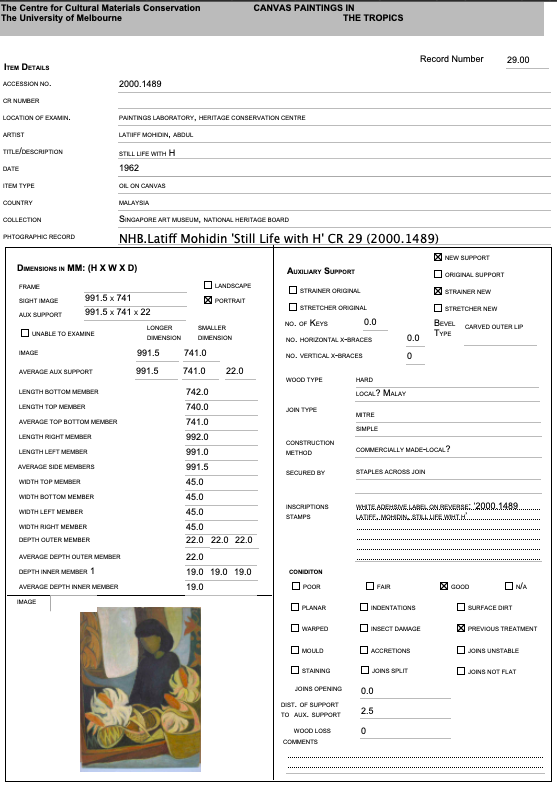
\includegraphics[width=0.9\textwidth]{images/ReportExample.png} % first figure itself
        \caption{Example of a FileMaker Pro Condition Report}
        \label{fig:conditionReportEx}
    \end{minipage}\hfill
    \begin{minipage}{0.5\textwidth}
        \centering
        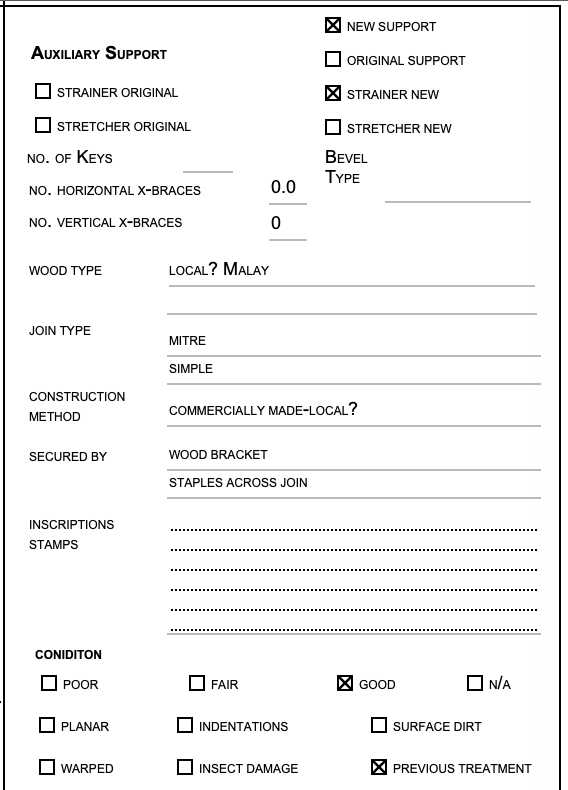
\includegraphics[width=0.9\textwidth]{images/zoomOnReportFields.png} % second figure itself
        \caption{Zoom on the auxiliary support part}
        \label{fig:zoomOnAuxiliary Report}
    \end{minipage}
\end{figure}

\noindent A condition report starts with general information such as the painting’s accession number (identifier of the painting), the name of the painting, the name of the artist, the country and the museum collection it belongs to, the dimensions and a thumbnail of the painting if available. It then focuses on the condition of every main component of the piece of art: the auxiliary support, the painting support, the ground layer, the painting layer, the surface coating and some miscellaneous information.
\bigbreak
\noindent For each of these main components, the report offers a large number of attributes that need to be filled in by the author of the report. There are two different types of attributes: they can either be text fields that the reporter can fill or boxes that can be ticked. An example for the text fields would be the ``comment” attribute from the auxiliary support, and one for the boxes would be the condition (poor, fair, good, excellent or N/A) of the ground layer shown in Figure \ref{fig:zoomOnAuxiliary Report}.
\bigbreak
\noindent However, the FileMaker Pro file is not directly usable in the data preprocessing pipeline. It was exported into an excel file using the ``export to excel” option from FileMaker Pro. Unfortunately, the excel file could not directly be used either. Indeed, it presented two types of problem:

\begin{itemize}
    \item Some of the exported values were just not correct as shown in the red rectangle in Figure \ref{FMPexport}.
    \item Categorical and ordinal variable that have several possible values were exported as separated variables in the excel file (cf. blue rectangle in Figure \ref{FMPexport})
\end{itemize}

\begin{figure}[H]
    \centering
    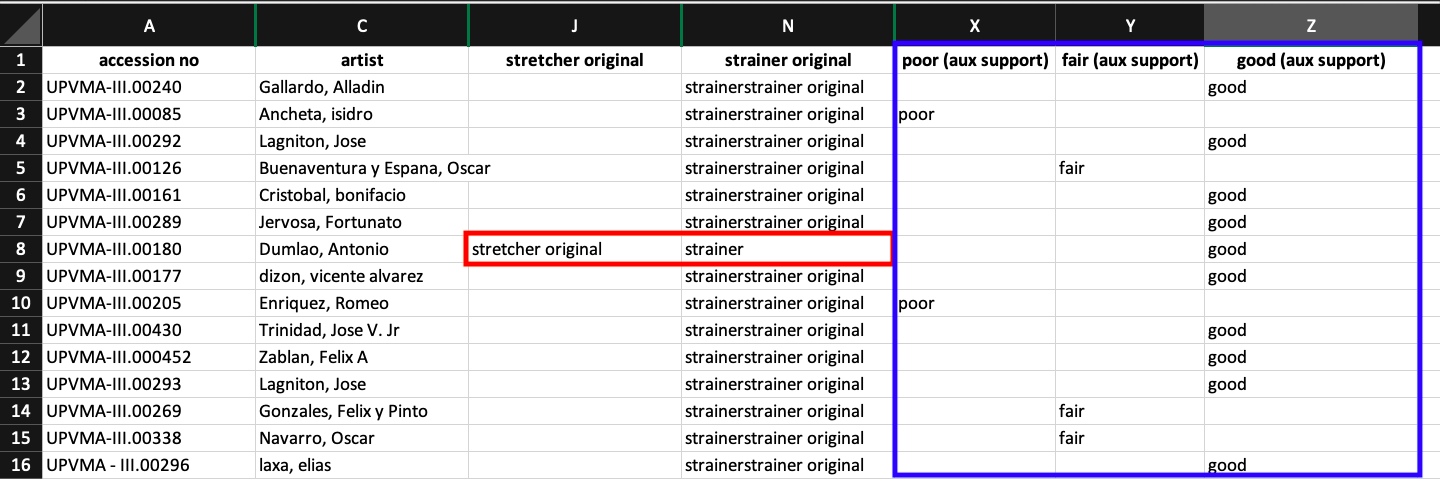
\includegraphics[width=0.99\textwidth]{images/exportFMP.png}
    \caption{raw export from FileMakerPro}
    \label{FMPexport}
\end{figure}

\noindent We could not find any explanation nor any pattern for the first problem even after discussion with the client. This resulted in the impossibility to implement an algorithm to solve it. Therefore, we had to clean it manually by correcting all the explainable export errors and the typos due to manual entries. To do that, each member was assigned a section of the raw excel file and we had to correct these typos or pieces of text that were not supposed to be here. We ended up with a manually cleaned excel file that we could process using a python script (cf. Figure \ref{ManCleanD})

\begin{figure}[H]
    \centering
    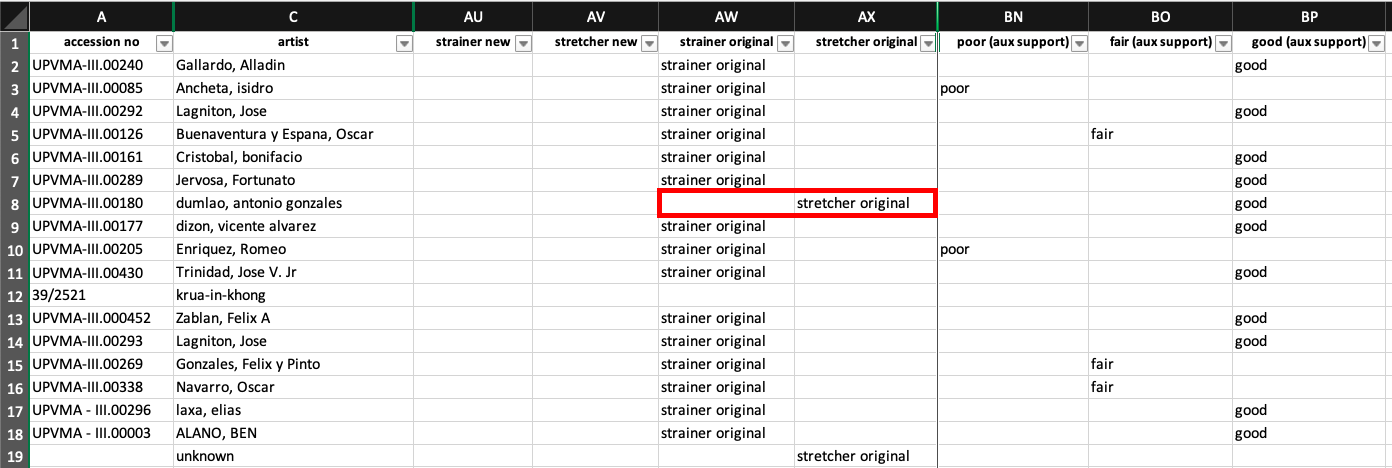
\includegraphics[width=0.99\textwidth]{images/ManCleanDSProject.png}
    \caption{manually cleaned data}
    \label{ManCleanD}
\end{figure}


\subsection{Metadata}
\begin{figure}[H]
    \centering
    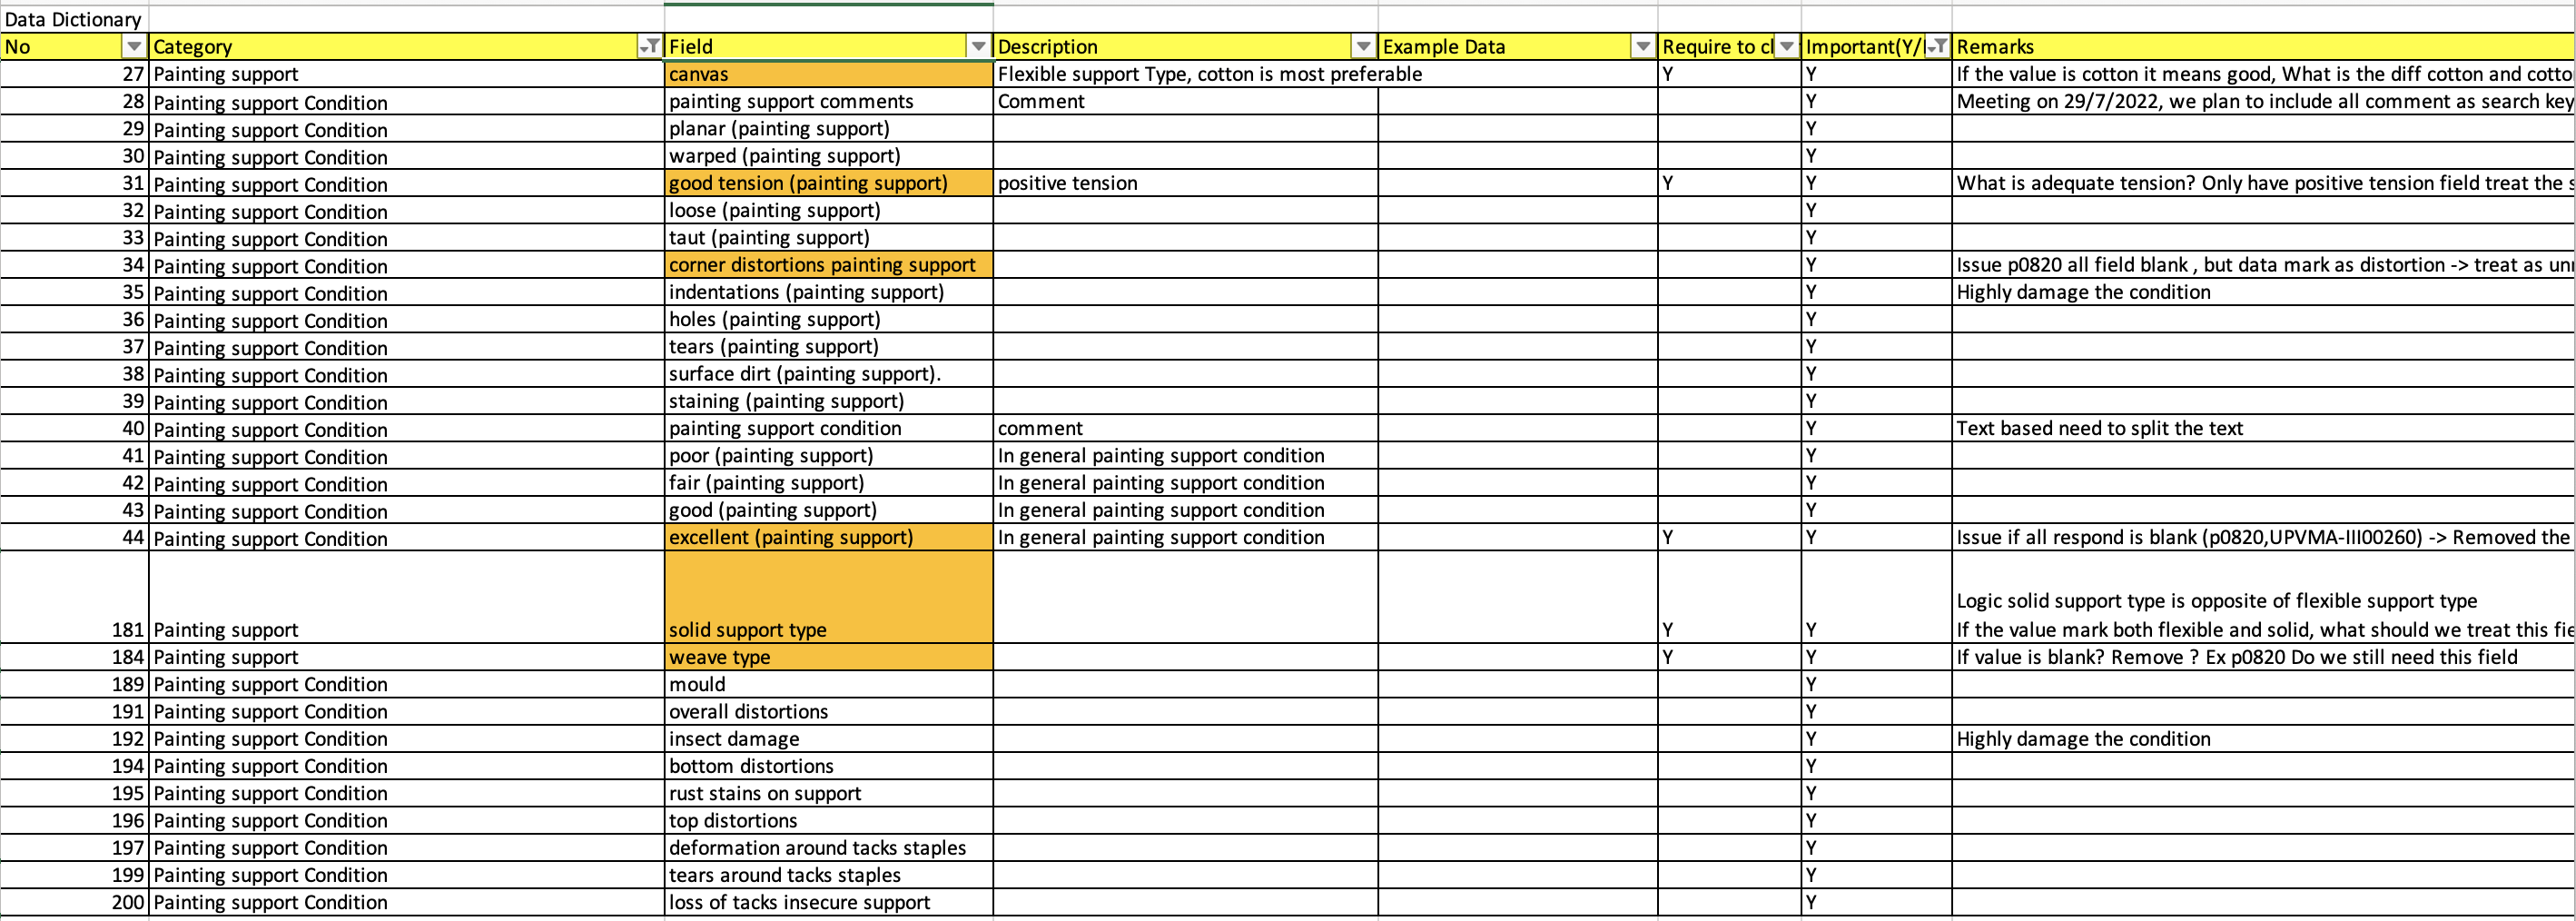
\includegraphics[scale=0.3]{images/Data_dict.png}
    \caption{Metadata}
    \label{Data_dict}
\end{figure}
We have also developed metadata for the given dataset, shown in Figure \ref{Data_dict}, to summarise information on each data field. Each field would collect the index of a feature from the exported CSV file since we found out that the columns fields were not sorted correctly. We also described the logic of some essential fields in order to analyse them when we did some in-depth analysis. Hence, our team could locate and work with particular attributes easier. 

\subsection{Preprocessing Steps}

The preprocessing script had two goals :
\begin{enumerate}
    \item Select the columns we needed for the dashboard only
    \item Reduce the number of features by fusing the columns that represented the same categorical/ordinal data
\end{enumerate}

\medbreak
\noindent In order to do it, we first created four python dictionaries at the beginning of the script. Each dictionary had keys which were the names of the final features we had selected, the argument of the keys would depend on the dictionary.
Two dictionaries are represented in figure \ref{dictionaries}, the complete list is :
\begin{itemize}
    \item \texttt{BooleanColumnsDict} : A dictionary for which the argument of each key is the position of the column in the manually cleaned file.
    \item \texttt{CategoricalColumnsDict} : A dictionary for categorical data. The argument of each key is a list of column indexes representing all the columns in the manually cleaned file that refer to the same categorical feature.
    \item \texttt{MultipleValuesCatColDict}:
    A dictionary for columns that represented several categorical values in a single cell. The argument of each key is a tuple presenting the index of the original cell, the maximum number of values that are in the original cell and the list of all possible values.
    \item \texttt{OrdinalColumnsDict}: A dictionary for ordinal data. The argument of each key is a list of column indexes representing all the columns in the manually cleaned file that refer to the same ordinal feature. The indexes are sorted from the lowest ordinal value to the highest.
\end{itemize}

\begin{figure}[H]
    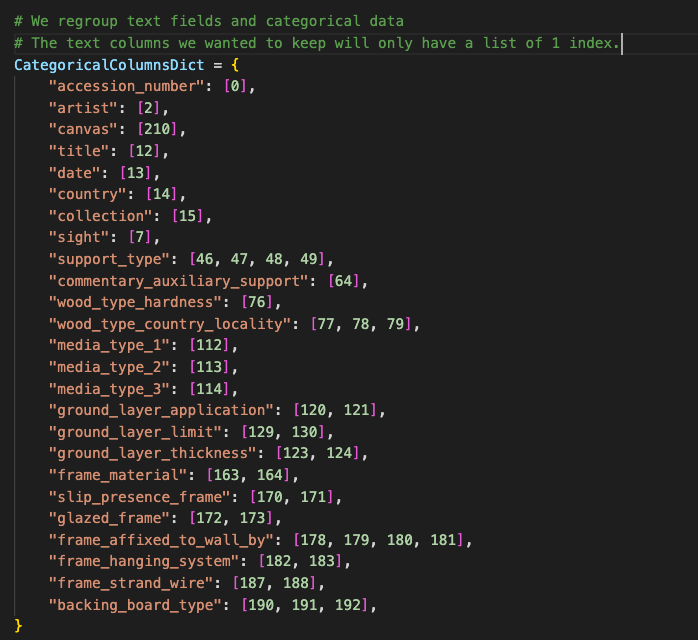
\includegraphics[width=0.45\textwidth]{images/catDic.png} \hfill
    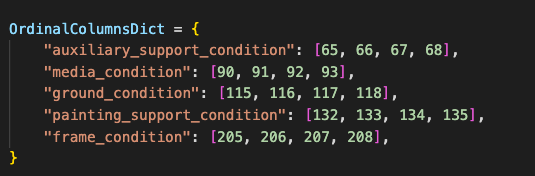
\includegraphics[width=0.45\textwidth]{images/ordDic.png} \hfill
    \caption{Example of dictionaries}
    \label{dictionaries}
\end{figure}

\noindent The first step in the preprocessing script was to fuse columns of the same categorical feature. This usually involved the fuction \texttt{fuseCategColumns} defined in Algorithm \ref{fuseCat}. There are five specific features that were treated differently :
\begin{itemize}
\item \texttt{canvas} : which was stripped of all the information that was not directly the canvas type (leaving only the values: \texttt{cotton}, \texttt{linen} or \texttt{bast})
\item \texttt{wood\_type\_country\_locality} :  which was separated into three new columns \texttt{wood\_type}, \texttt{wood\_country} and \texttt{locality}
\item \texttt{collection} :  because the names of each collection are changed from the raw data after a request from the client
\item \texttt{sight} : because it is used to create a \texttt{area} feature
\item \texttt{date} : which is used to create a \texttt{decade} feature
\end{itemize}

\noindent Then the code tackled \texttt{MultipleValuesCatColDict}. This consisted in creating a binary column for each possible value for this feature. This was done by checking in a \texttt{for} loop on the possible values if the long \texttt{string} in the original data contained the said value or not.
\bigbreak
\noindent After that the script fused together the ordinal data. This was done with \texttt{fuseOrdinalColumns}, the algorithm of which is described in annex \ref{fuseOrd}. It considered the columns in the original data that referred to the same ordinal feature and for a specific row it gave the level of the first non empty column it had encountered. If another column had a value, it then computed the mean with the former assigned level and took the closest upper integer. The lowest level was always 0 and the rows without any value were filled with NaNs.
\bigbreak
\noindent Finally, the script handled binary data. In the original dataframe, these columns were either filled with the name of the column itself when the attribute was present or they were left empty. The script only checked if for a given column some cells were empty or not. It then transformed empty cells into 0 and the others into 1.

\newpage
\section{Exploratory Data Analysis}
Exploratory data analysis is an important process to analyse and summarise the characteristic of a dataset. In this section, we will be exploring the provided dataset to present a general idea of the data that we are dealing with.

\subsection{How is the Data Distributed?}
In our analysis, we explored various categorical features of the dataset to get more depth about the data. First, we have explored the painting distribution across the four museums, as shown in Figure \ref{museum_dist}. We saw that the National Heritage Board of Singapore has the highest number of paintings at 63, followed by JB Vargas Museum and Balai Seni Negara of Malaysia. In comparison, the National Gallery of Thailand has the least number of paintings at 33.
\begin{figure}[H]
    \centering
    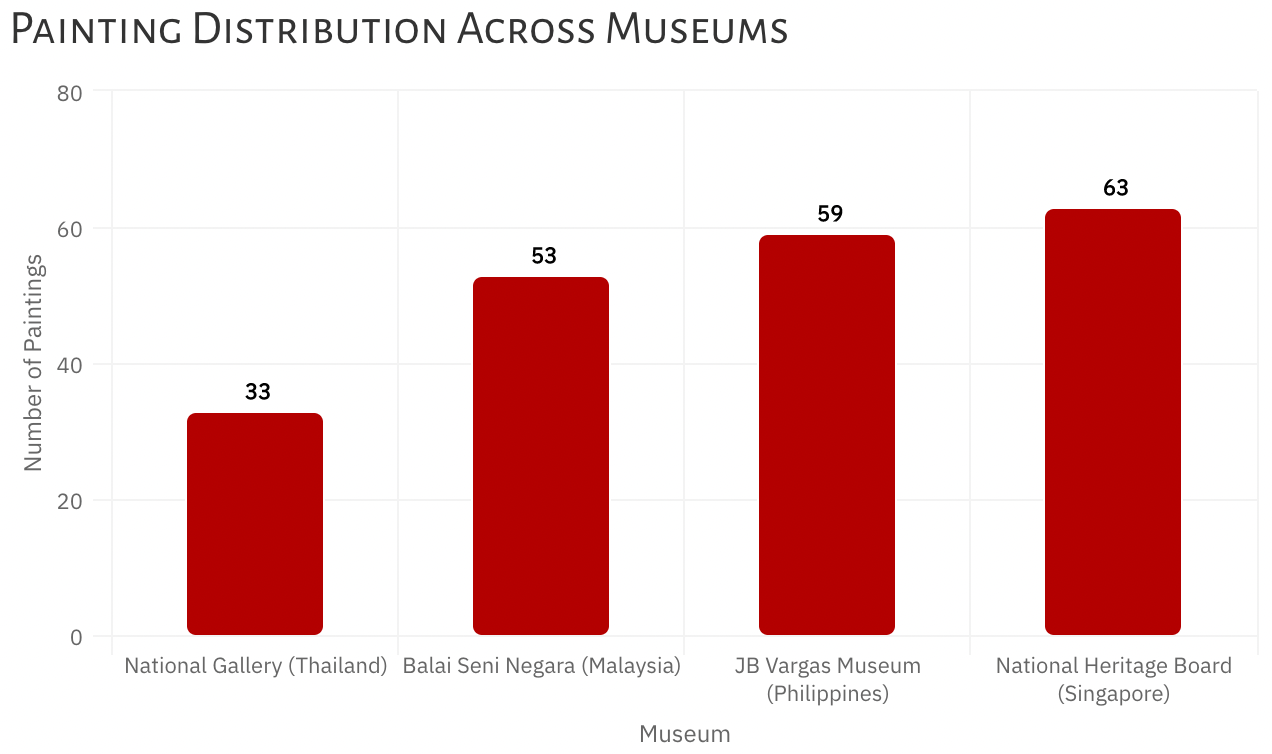
\includegraphics[scale=0.45]{images/museum_dist.png}
    \caption{Distribution of Paintings Across Museums}
    \label{museum_dist}
\end{figure}

\noindent Next, we explored the painting distribution across the timeline as shown in Figure \ref{time_dist}. We can observe that the distribution of the paintings were heavily left skewed as most of the paintings were between the 1930s and 1960s. Another point worth mentioning is that all the Balai Seni Begara (Malaysia) paintings were from after 1920.
\begin{figure}[H]
    \centering
    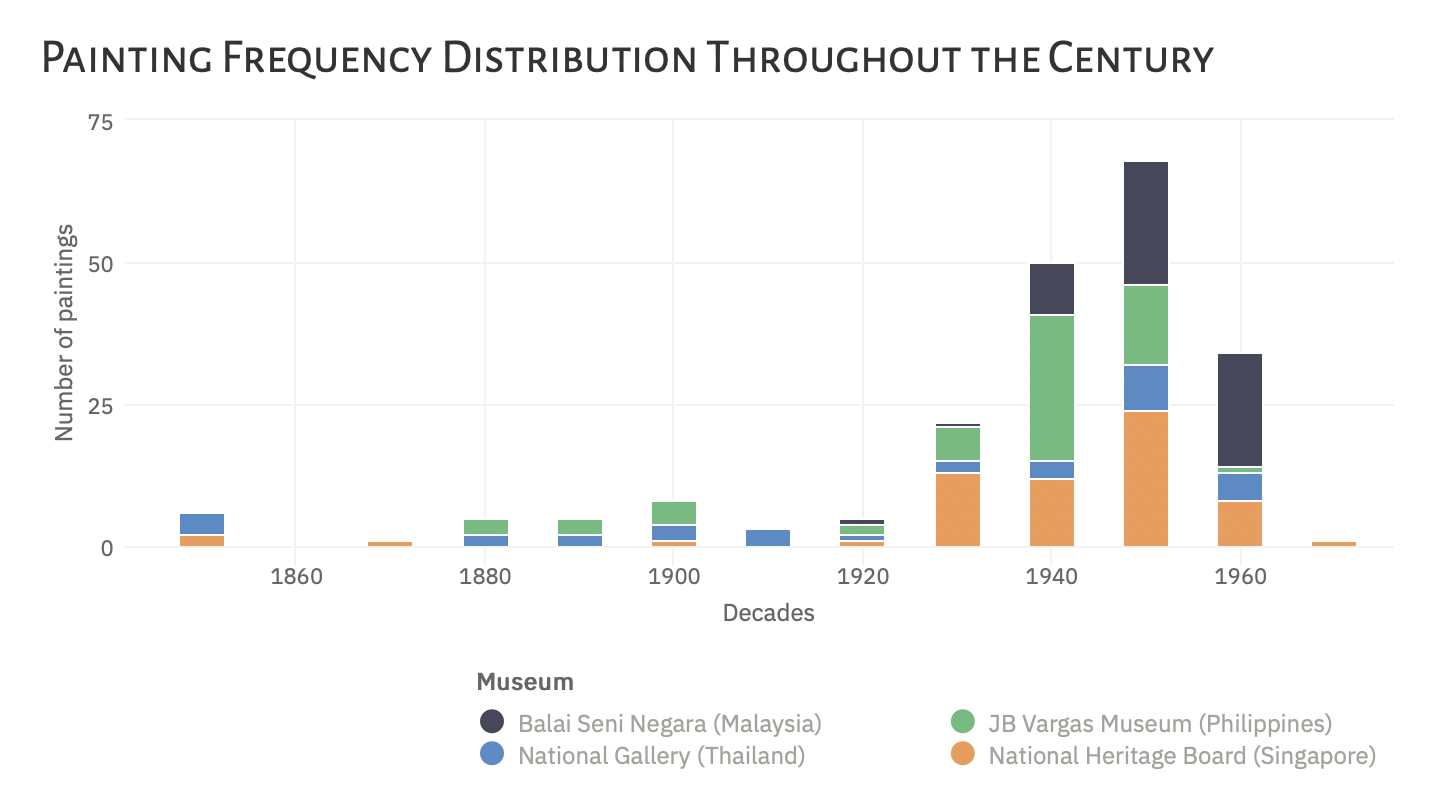
\includegraphics[scale=0.5]{images/time_dist.png}
    \caption{Distribution of Paintings Across the Timeline}
    \label{time_dist}
\end{figure}

\noindent In Figure \ref{canvas_material}, we explored the commonly used materials across all museums. Apart from the paintings with unspecified materials, we can see that the number of paintings with cotton canvas is significantly higher than other used fabrics in Balai Seni Negara and JB Vargas Museum. In contrast, the number of paintings with cotton or linen canvas is relatively the same in the National Gallery of Thailand and the National Heritage Board of Singapore.

\begin{figure}[H]
    \centering
    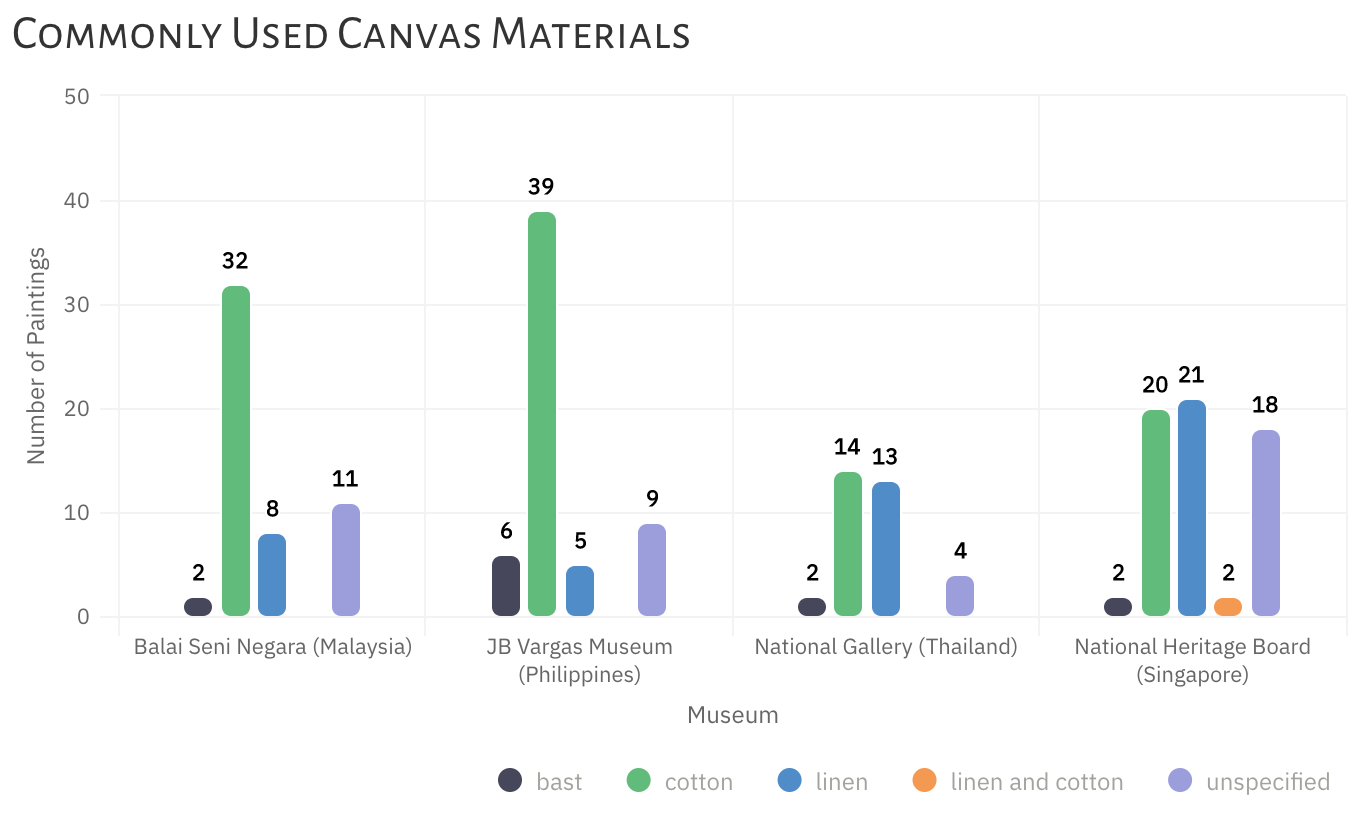
\includegraphics[scale=0.55]{images/canvas_material.png}
    \caption{Commonly Used Canvas Materials}
    \label{canvas_material}
\end{figure}

\noindent Moreover, Figure \ref{media_material} shows that oil paint is the most popular media/paint materials across the four museums. As over 90\% of all paintings were painted with oil.

\begin{figure}[H]
    \centering
    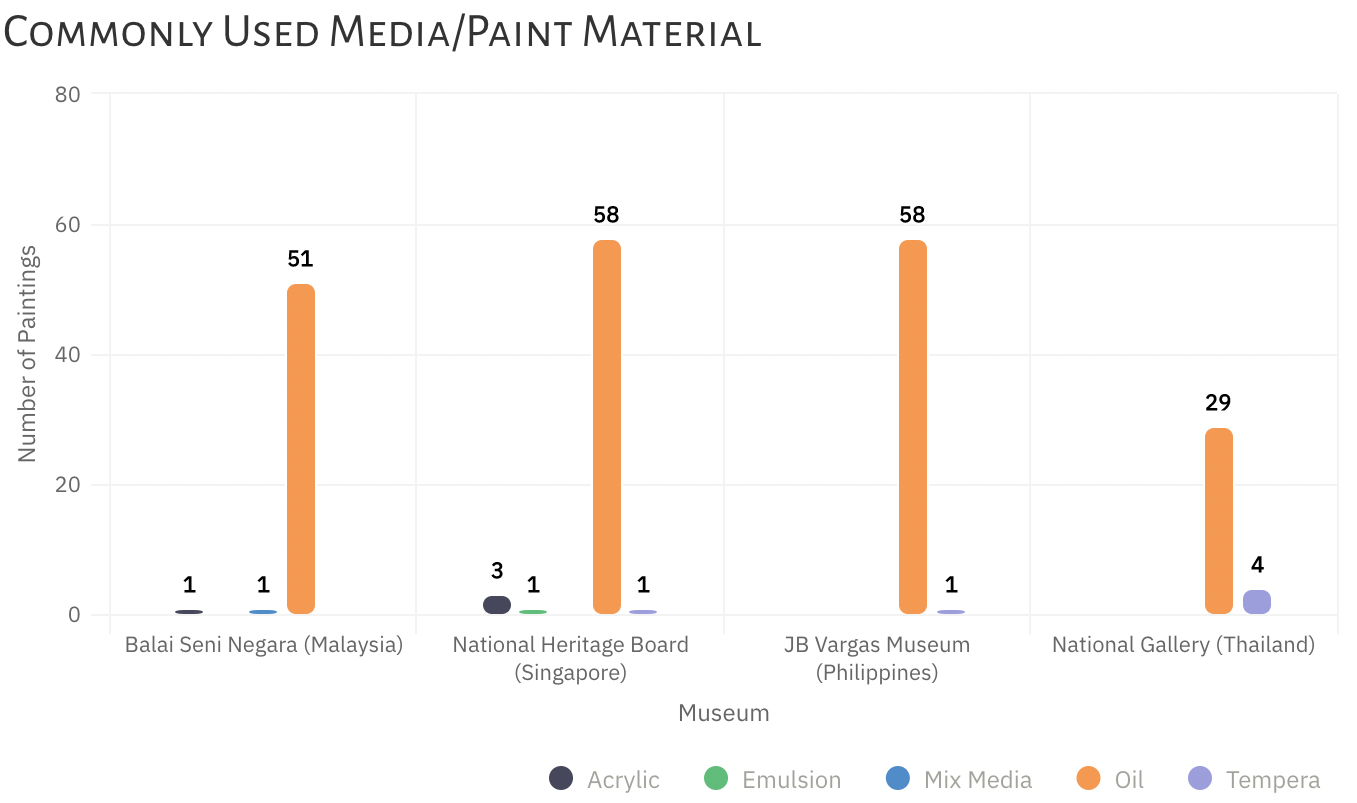
\includegraphics[scale=0.55]{images/media_material.png}
    \caption{Commonly Used Media/Paint Materials}
    \label{media_material}
\end{figure}

\noindent Furthermore, we have explored the distribution of ground type as shown in Figure \ref{ground_type}. Apart from the paintings with unspecified or unsure ground type, we can see that over 60\% of paintings' ground layers in the National Heritage Board were commercially applied. In contrast, 59\% of paintings from Balai Seni Negara has artist applied ground. While the number of paintings with commercial applied or artist applied ground is relatively the same for JB Vargas Museum and the National Gallery of Thailand.

\begin{figure}[H]
    \centering
    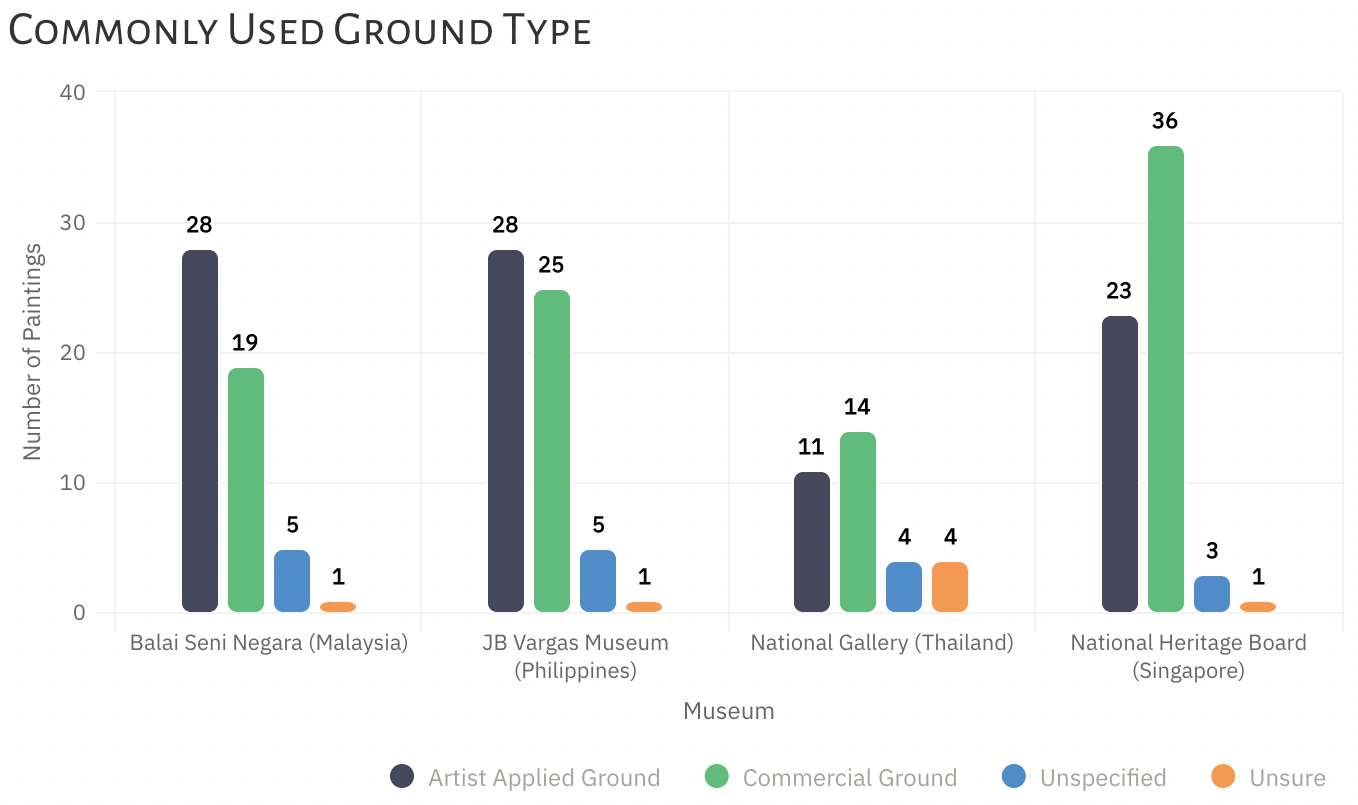
\includegraphics[scale=0.5]{images/ground_type.png}
    \caption{Commonly Used Ground Type}
    \label{ground_type}
\end{figure}

\subsection{How is the Condition Rating of Paintings from each Museum?}
As mentioned in the project domain section, paintings generally consist of five components. A condition rating score (Poor, Fair, Good, or Excellent) was assigned to each component of the painting by the client during the study. Here we explored the condition rating distribution for each museum to get more depth about the data.
\subsubsection{Auxiliary Support Condition Rating}
\begin{figure}[H]
    \centering
    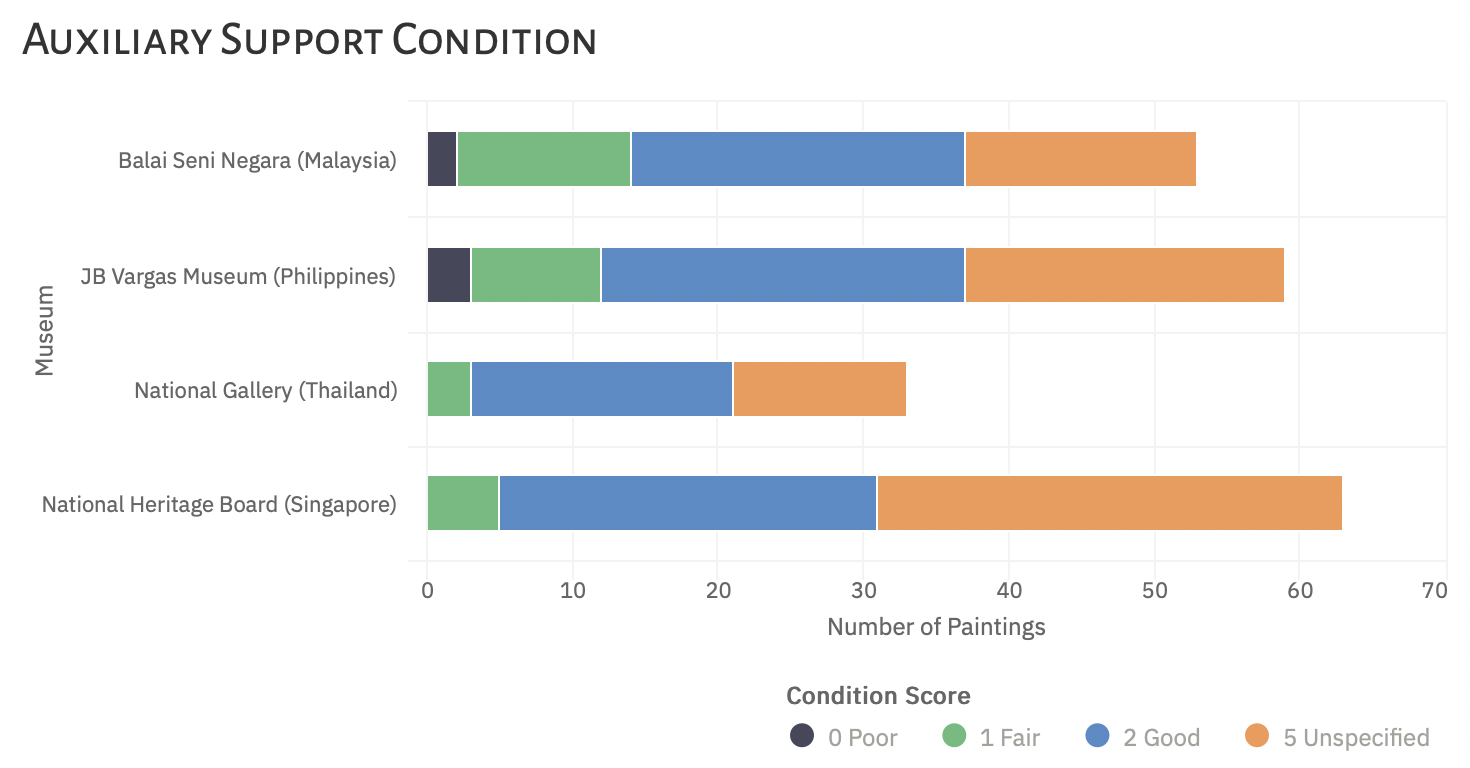
\includegraphics[scale=0.5]{images/aux_cond.png}
    \caption{Auxiliary Support Condition Overview}
    \label{aux_cond}
\end{figure}
As per the stacked bar chart shown in Figure \ref{aux_cond}, each museum has a fair amount of paintings with an unspecified condition score for auxiliary support. This is either because the auxiliary support could not be evaluated or because the piece of art did not present any sort of auxiliary support. Moreover, each museum has approximately the same amount of paintings in good condition for auxiliary support, and no paintings with an excellent rating can be found. However, we notice a few paintings from JB Vargas Museum and Balai Seni Negara that were assigned to poor.

\subsubsection{Paint Support Condition Rating}
\begin{figure}[H]
    \centering
    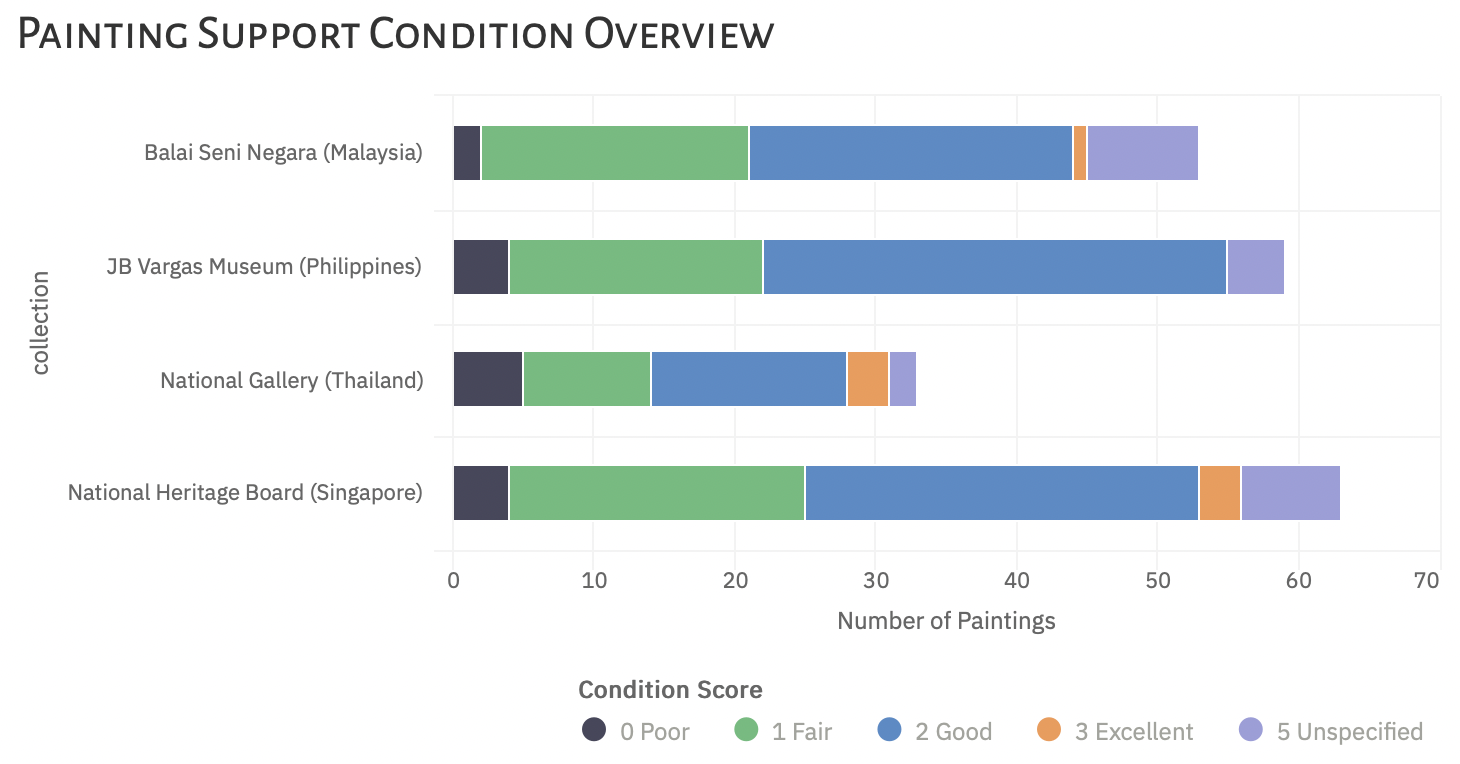
\includegraphics[scale=0.5]{images/support_cond.png}
    \caption{Paint Support Condition Overview}
    \label{support_cond}
\end{figure}
As for the paint support condition shown in Figure \ref{support_cond}, painting with unspecified ratings were found across all the museums. And we saw that most paintings were assigned with a fair and good condition for paint support, while only a tiny portion of paintings was assigned to poor or excellent.

\subsubsection{Ground Layer Condition Rating}
\begin{figure}[H]
    \centering
    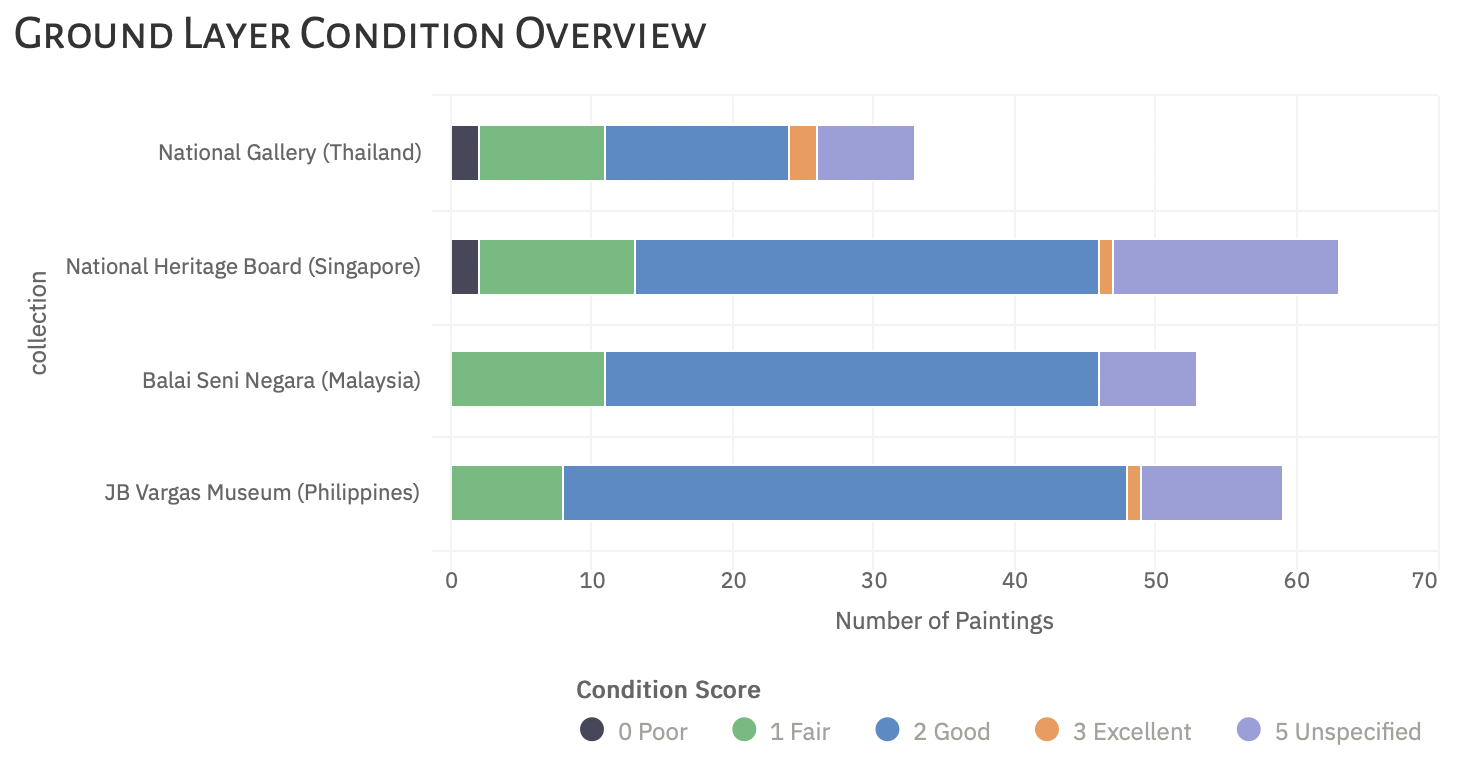
\includegraphics[scale=0.5]{images/ground_cond.png}
    \caption{Ground Layer Condition Overview}
    \label{ground_cond}
\end{figure}
The ground layer condition of the paintings across the museum were shown in Figure \ref{ground_cond}. Again, paintings with unspecified ground ratings were found across each museum. We saw that most of paintings were clustered between fair and good. Only a tiny portion of paintings were classified as poor or excellent.

\subsubsection{Paint/Media Layer Condition Rating}
Similarly, we have created a stacked bar chart showing the number of paintings in each museum based on their paint layer condition which is shown in Figure \ref{media_cond}. Paintings with unspecified paint layer condition can be observed across all museums. The story is relatively the same with previous layers, where most paintings were classified with fair and good ratings. It is also worth noting that most paintings with excellent ratings were from the National Heritage Board of Singapore, while the number of paintings with poor ratings in the National Gallery of Thailand are relatively higher than the other museums.
\begin{figure}[H]
    \centering
    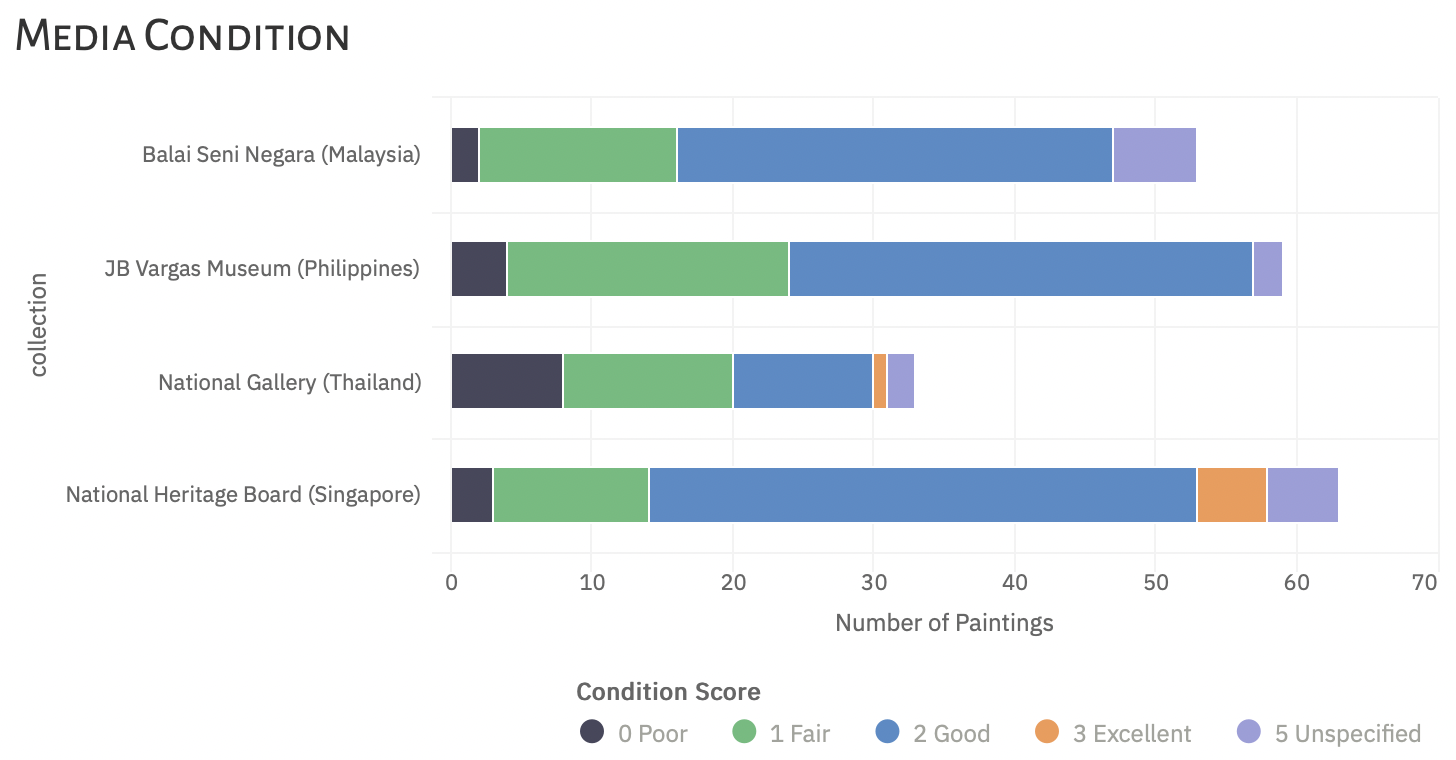
\includegraphics[scale=0.5]{images/media_cond.png}
    \caption{Paint/Media Layer Condition Overview}
    \label{media_cond}
\end{figure}

\subsubsection{Frame Condition Rating}
\begin{figure}[H]
    \centering
    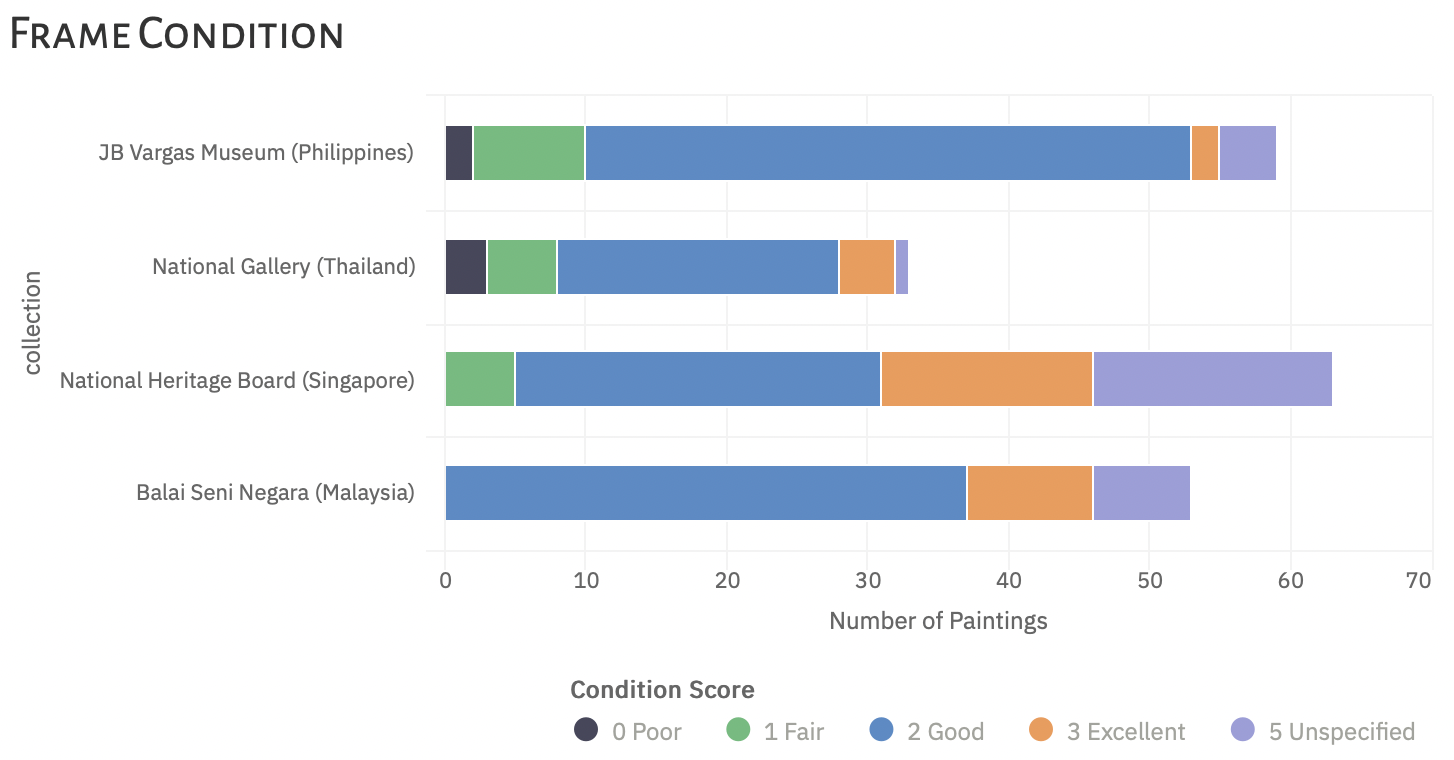
\includegraphics[scale=0.5]{images/frame_cond.png}
    \caption{Frame Condition Overview}
    \label{frame_cond}
\end{figure}
Frame condition across the four museums is shown in Figure \ref{frame_cond}. Paintings with unspecified frame condition can be identify across all museums, which is either missed or does not consist of a frame. We observed that the number of paintings with unspecified frame condition are comparatively higher in the National Heritage Board of Singapore. And it is noteworthy that the portion of paintings with excellent condition is considerably higher than other component mentioned above.

\subsection{How is the Painting Condition Among the Museums?}
As discussed with the client, the client provided the scope of requirements to the team to explore the condition attributes on paint support, ground layer, and paint layer rather than auxiliary support and frame, given that the client is more interested in those layers. Here, we have selected a few condition attributes of those layers to explore their general distribution among the museums.

\subsubsection{Holes Condition}
\begin{figure}[H]
    \centering
    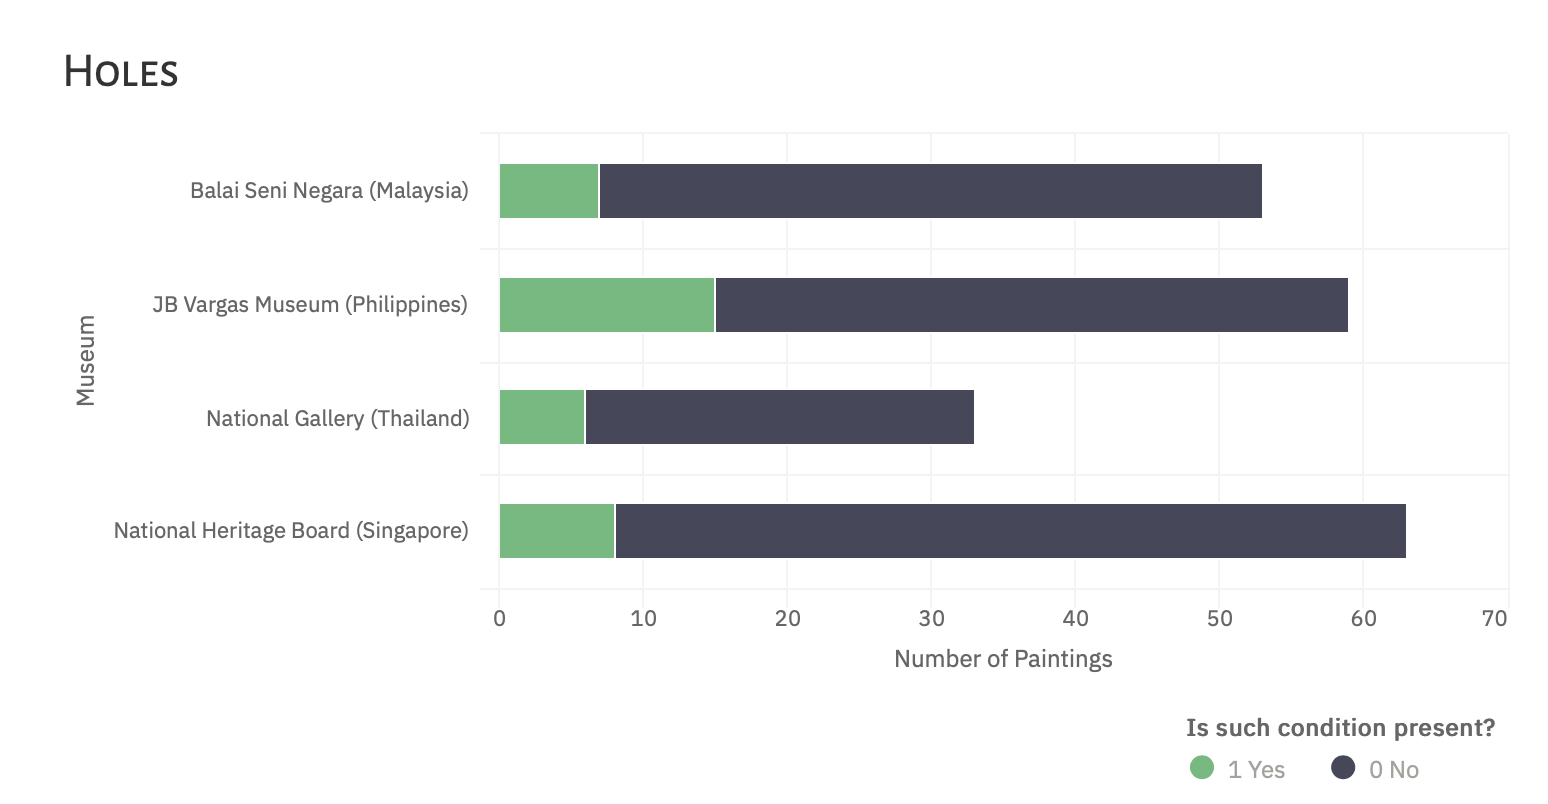
\includegraphics[scale=0.5]{images/Holes_painting_con.png}
    \caption{Holes condition}
    \label{Holes_painting_con}
\end{figure}
As the Holes condition stacked bar chart shown in Figure \ref{Holes_painting_con}, each museum has a similar amount of holes condition. In contrast, JB Vargas museum has nearly double the holes condition of other museums (15 paintings).

\subsubsection{Positive Tension Condition}
\begin{figure}[H]
    \centering
    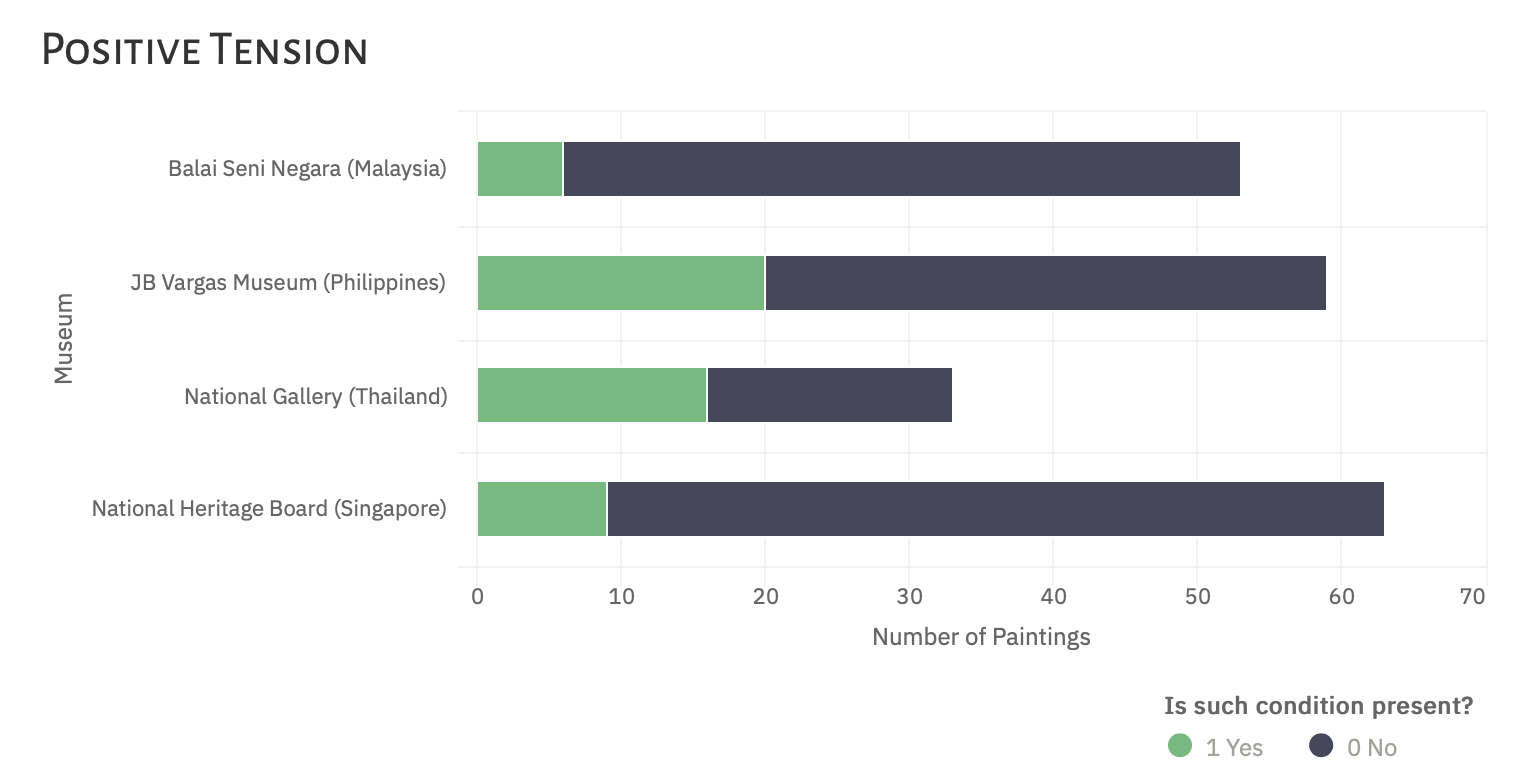
\includegraphics[scale=0.5]{images/Positive_Ten_painting_con.png}
    \caption{Positive Tension condition}
    \label{Positive_Ten_painting_con}
\end{figure}
As the Positive Tension condition stacked bar chart shown in Figure \ref{Positive_Ten_painting_con}, Balai Seni Negara (Malaysia) and National Heritage Board (Singapore) have a similar amount of Positive tension condition. In contrast, JB Vargas museum and National Gallery (Thailand) have nearly double the holes condition of other museums (20 and 16 paintings, respectively).

\subsubsection{Are Ground layer Thinly or Thickly Applied}
\begin{figure}[H]
    \centering
    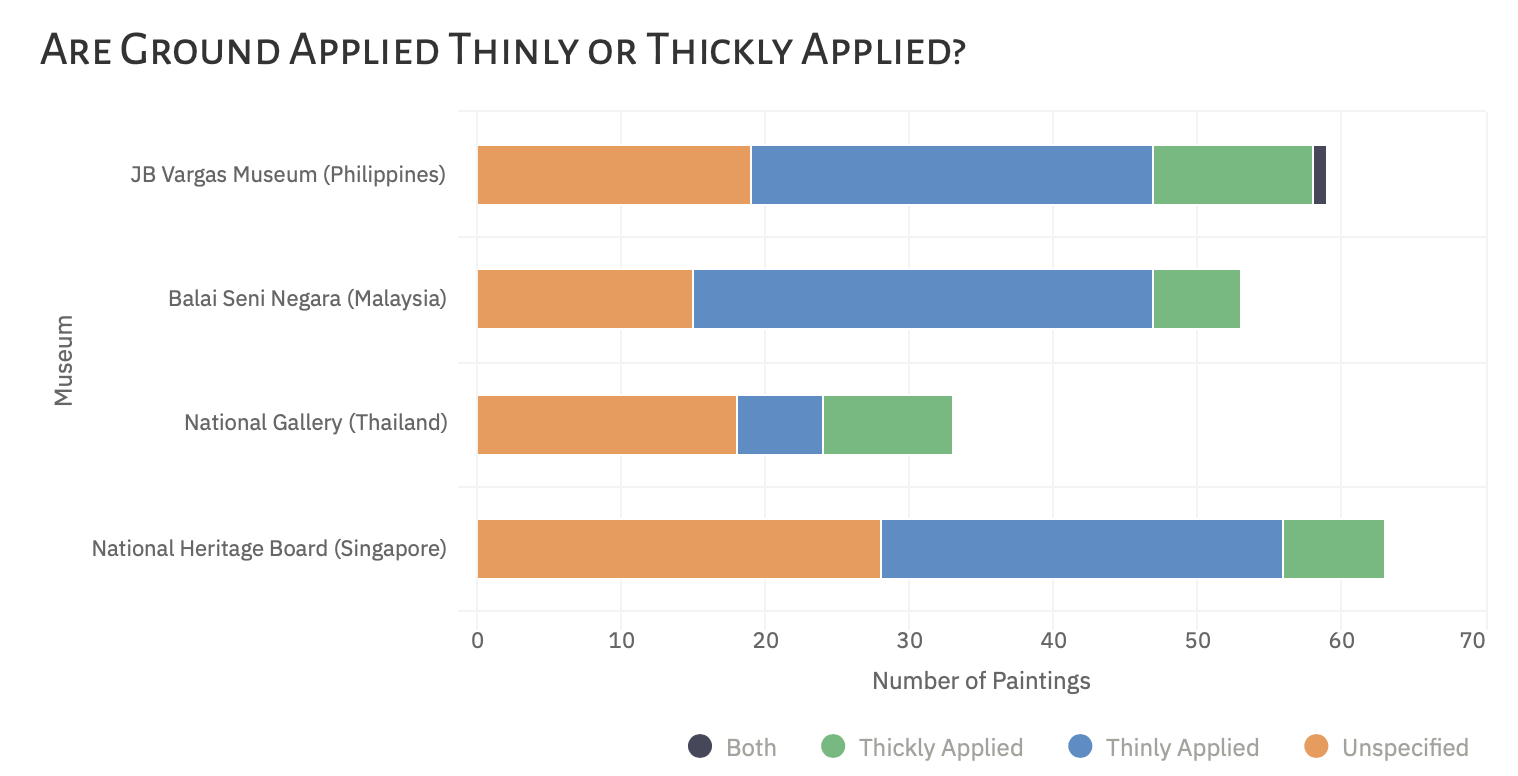
\includegraphics[scale=0.5]{images/ThinVsThick_Ground_con.png}
    \caption{Are ground layer Thinly or Thickly Applied}
    \label{ThinVsThick_Ground_con}
\end{figure}
As the ground layer Thinly or Thickly Applied condition stacked bar chart shown in Figure \ref{ThinVsThick_Ground_con}, most museums have Thinly applied rather than Thickly applied expecting Nation Gallery (Thailand). However, we found that unspecified conditions are significant huge among collections. Therefore, our team was inquisitive about filling unspecified conditions by predictive models.


\subsubsection{Uniform application}
\begin{figure}[H]
    \centering
    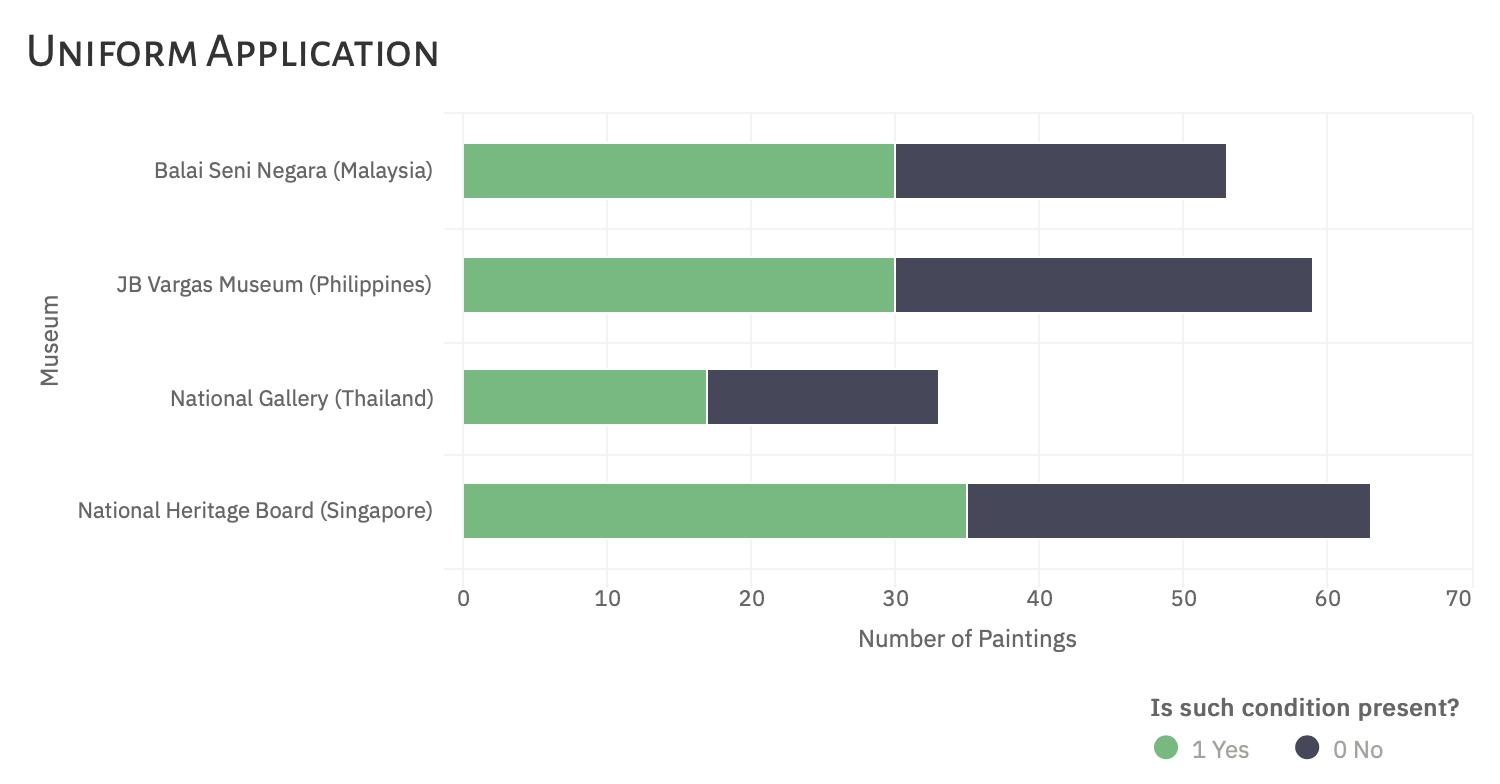
\includegraphics[scale=0.5]{images/Uniform_app_ground_con.png}
    \caption{Uniform application}
    \label{Uniform_app_ground_con}
\end{figure}
According to the stacked bar chart as shown in Figure \ref{Uniform_app_ground_con}, Every museum has a similar proportion of yes and no for uniform application. Our team suspected this condition is related to other conditions such as ground type, Thinly or Thickly Applied ground.

\subsubsection{Painting Plastic Behaviour}
\begin{figure}[H]
    \centering
    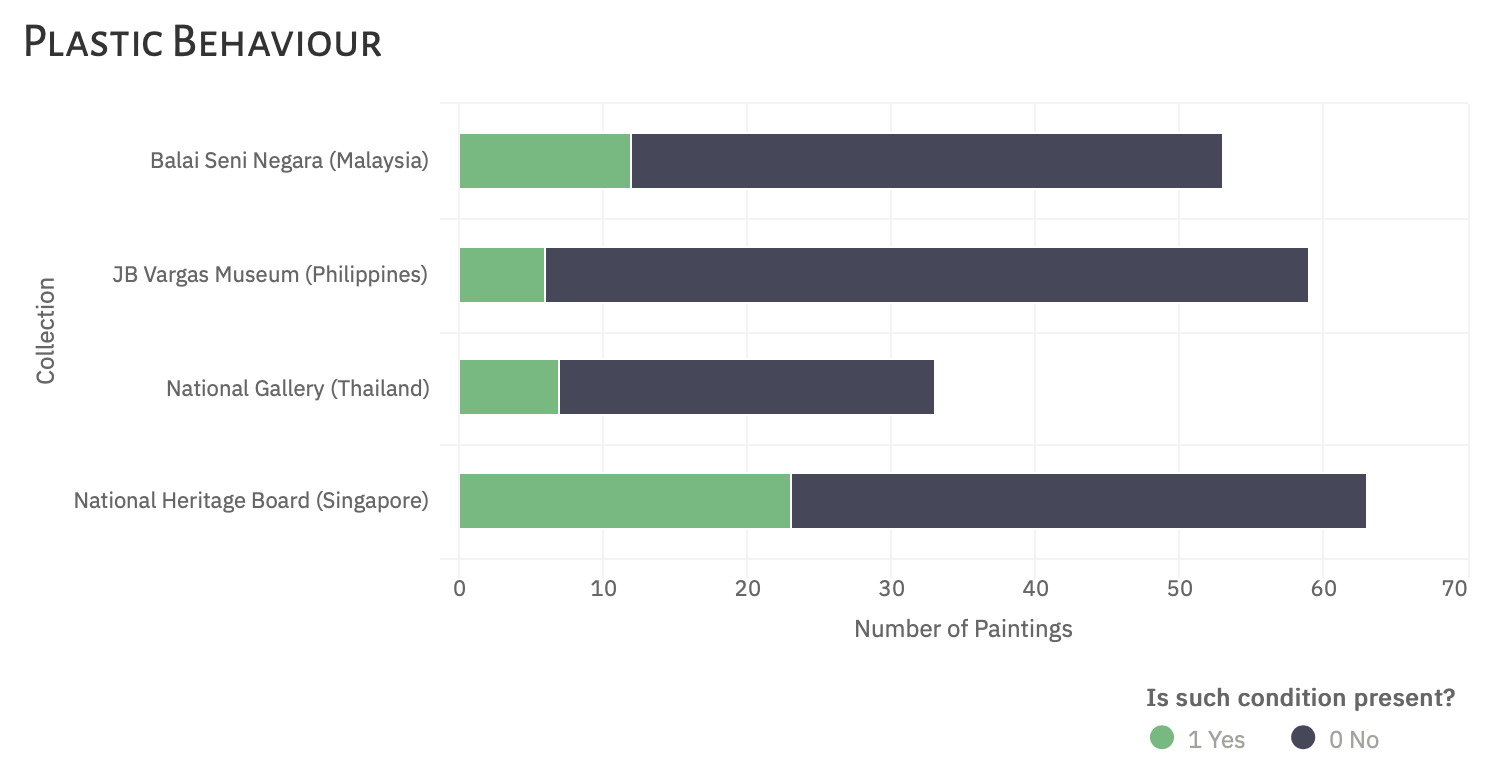
\includegraphics[scale=0.5]{images/Plastic_media_con.png}
    \caption{Plastic Behaviour}
    \label{Plastic_media_con}
\end{figure}
According to the stacked bar chart as shown Figure \ref{Plastic_media_con}, National Heritage Board (Singapore) has the most Plastic Behaviour on paintings layers among collections, 23 paintings. In contrast, the JB Vargas Museum and National Gallery (Thailand) have minor Plastic Behaviour on layers 6 and 7, respectively.
In addition, we examined the relationship with the painting layer condition. We discovered that there is an opposite relationship with painting layer condition when painting appears Plastic Behaviour is less likely to have good conditions.

\subsubsection{Painting Elastic Behaviour}
\begin{figure}[H]
    \centering
    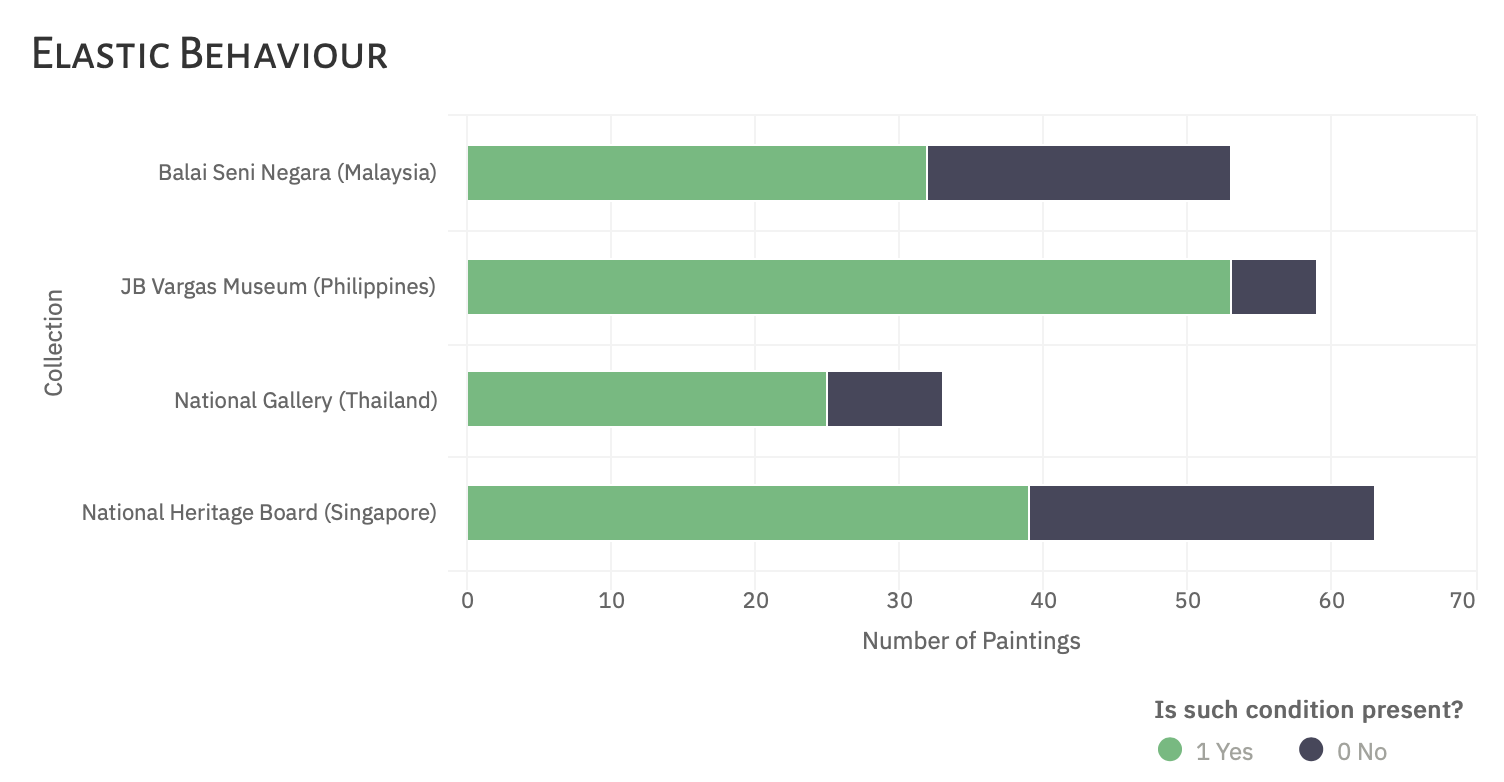
\includegraphics[scale=0.5]{images/Elastic_media_con.png}
    \caption{Elastic Behaviour}
    \label{Elastic_media_con}
\end{figure}
As the Elastic Behaviour condition stacked bar chart shown in Figure \ref{Elastic_media_con}, most museums present Elastic Behaviour. Furthermore, JB Vargas Museum has the most Elastic Behaviour condition on 53 paintings.
In addition, we examined the relationship with the painting layer condition. We discovered that there is a positive relationship with painting layer condition when painting appears Elastic Behaviour is more likely to have good conditions.

\section{Interactive Dashboard}
As discussed in the data preprocessing section, although FileMaker Pro is an excellent tool for collecting and recording data, it does not provide data visualisation for exploration and comparison. Therefore, transforming the given dataset and creating an interactive dashboard for the client has been our primary focus this semester. In this section, we will focus on covering our approach to creating the dashboard.

\subsection{Used Tools and Packages}
\textit{R Shiny}, \textit{Leaflet}, \textit{Highcharter}, and \textit{Polished} are the four main tools we make use of when implementing the dashboard. \textit{Shiny} is an R package that enables people to build interactive web interface straight from R, while the \textit{Leaflet} package enables us to deploy interactive map visualisation in the Shiny app. Moreover, the \textit{Highcharter} package allows us to add interactivity into visualisation figure to display more information when the user interacts with the plot. Finally, the \textit{Polished} package allows us to establish authentication to the Shiny application to ensure confidentiality.
\bigbreak
\noindent Along the way, we also considered tools like Tableau. However, to increase the technical challenge of this project, this idea was soon given up.

\subsection{Dashboard Design Summary}
\subsubsection{Homepage}
\begin{figure}[H]
    \centering
    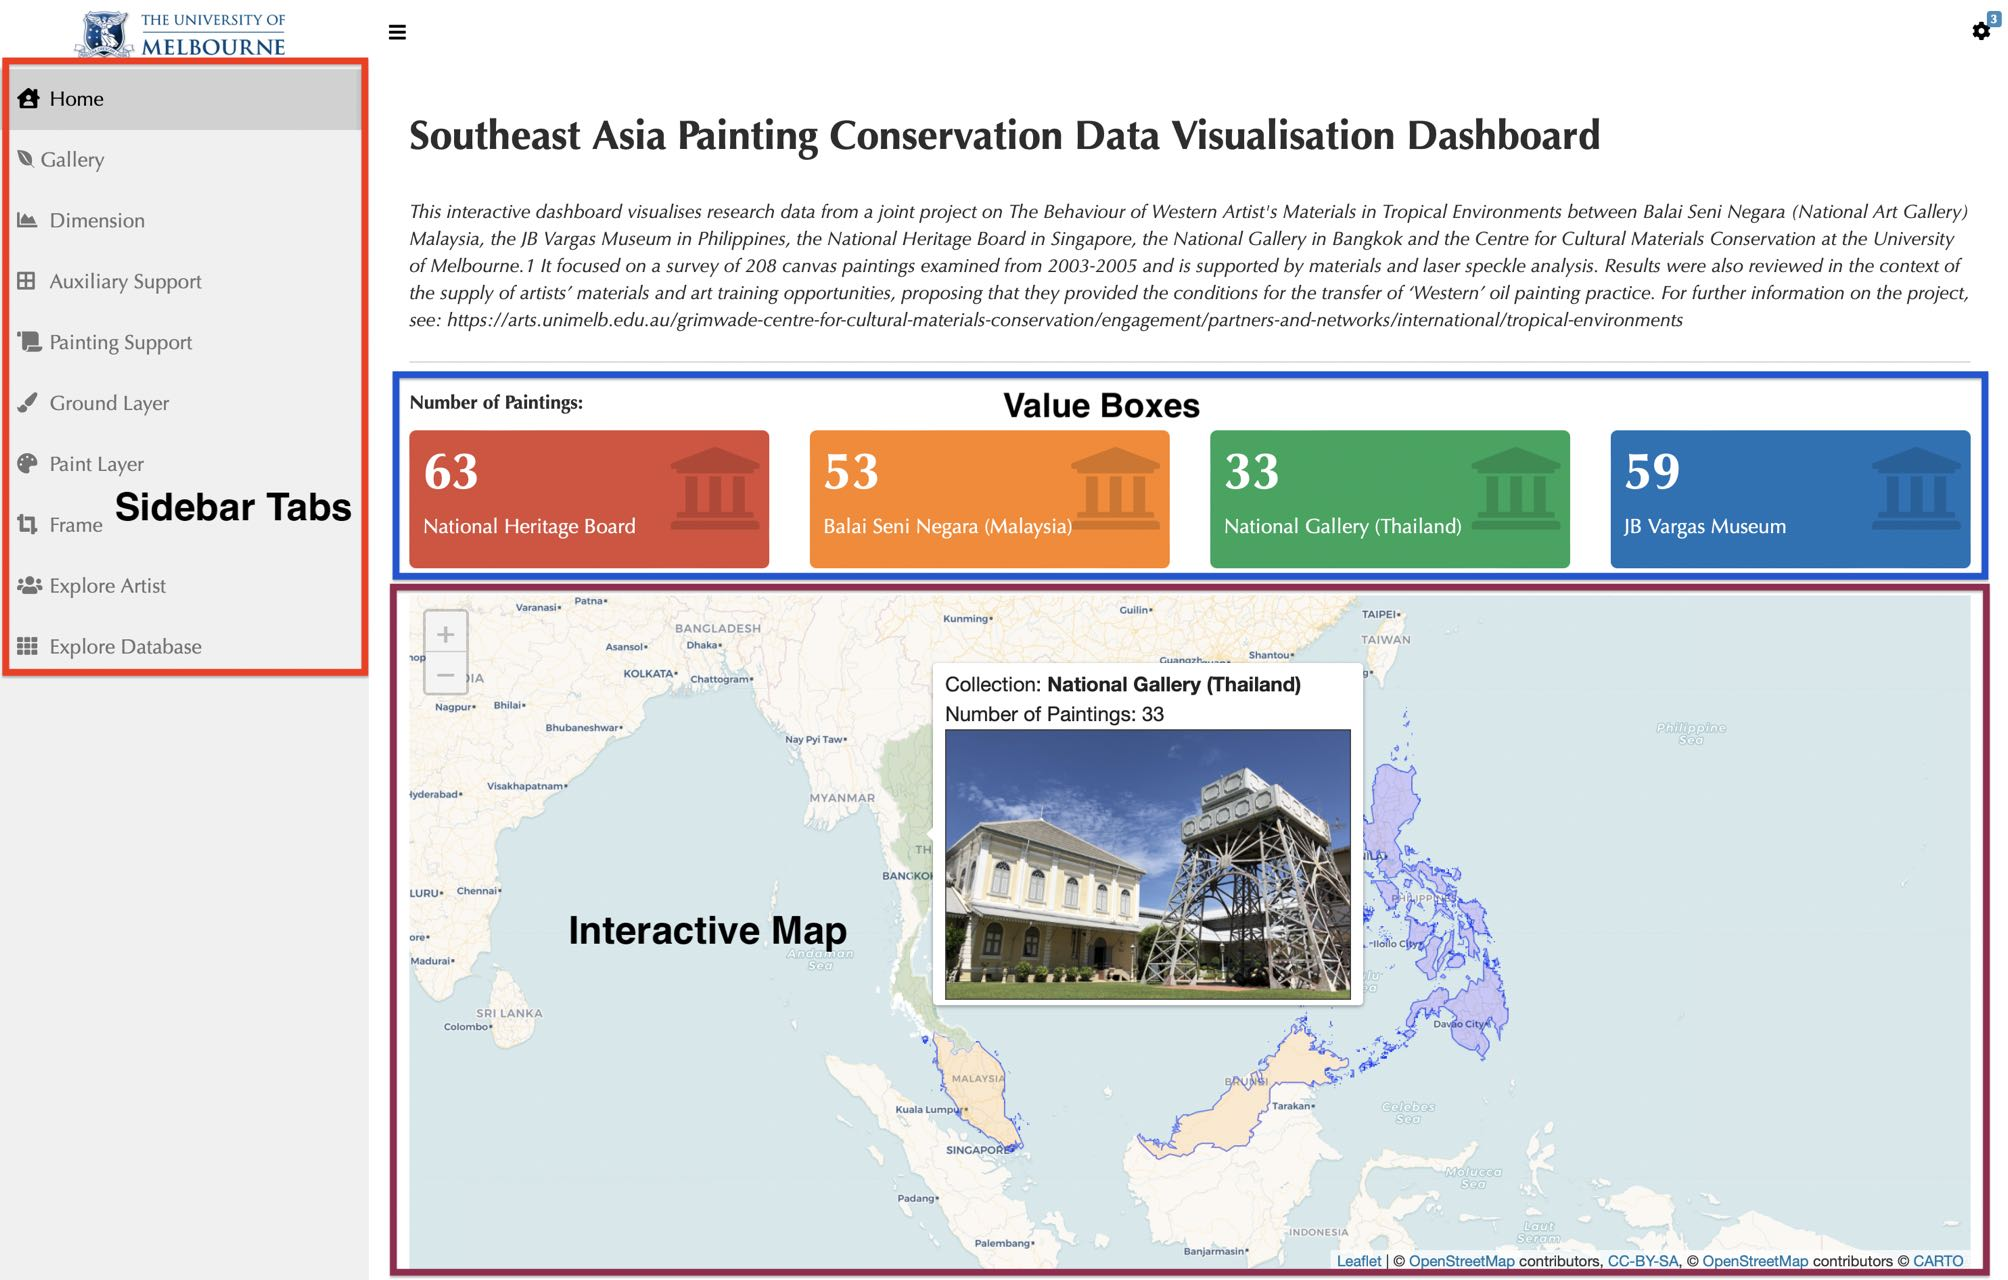
\includegraphics[scale=0.2]{images/Dashboard Homepage Screenshot.png}
    \caption{Dashboard Homepage}
    \label{dashboard_home}
\end{figure}

Our dashboard homepage are shown in Figure \ref{dashboard_home}. The homepage displays general information about the study behind the dashboard. The value boxes on top show the number of paintings in each of the four museums. We also used an interactive map to highlight the country in which each museum is located. Moreover, when the user hovers the mouse over the highlighted country's polygon, the tooltip will display the museum name, the number of paintings that participated in the study, and the photo of the museum. Furthermore, the sidebar tabs on the left allow users to navigate to the section they want to view.

\subsubsection{The Gallery Tab}
\begin{figure}[H]
    \centering
    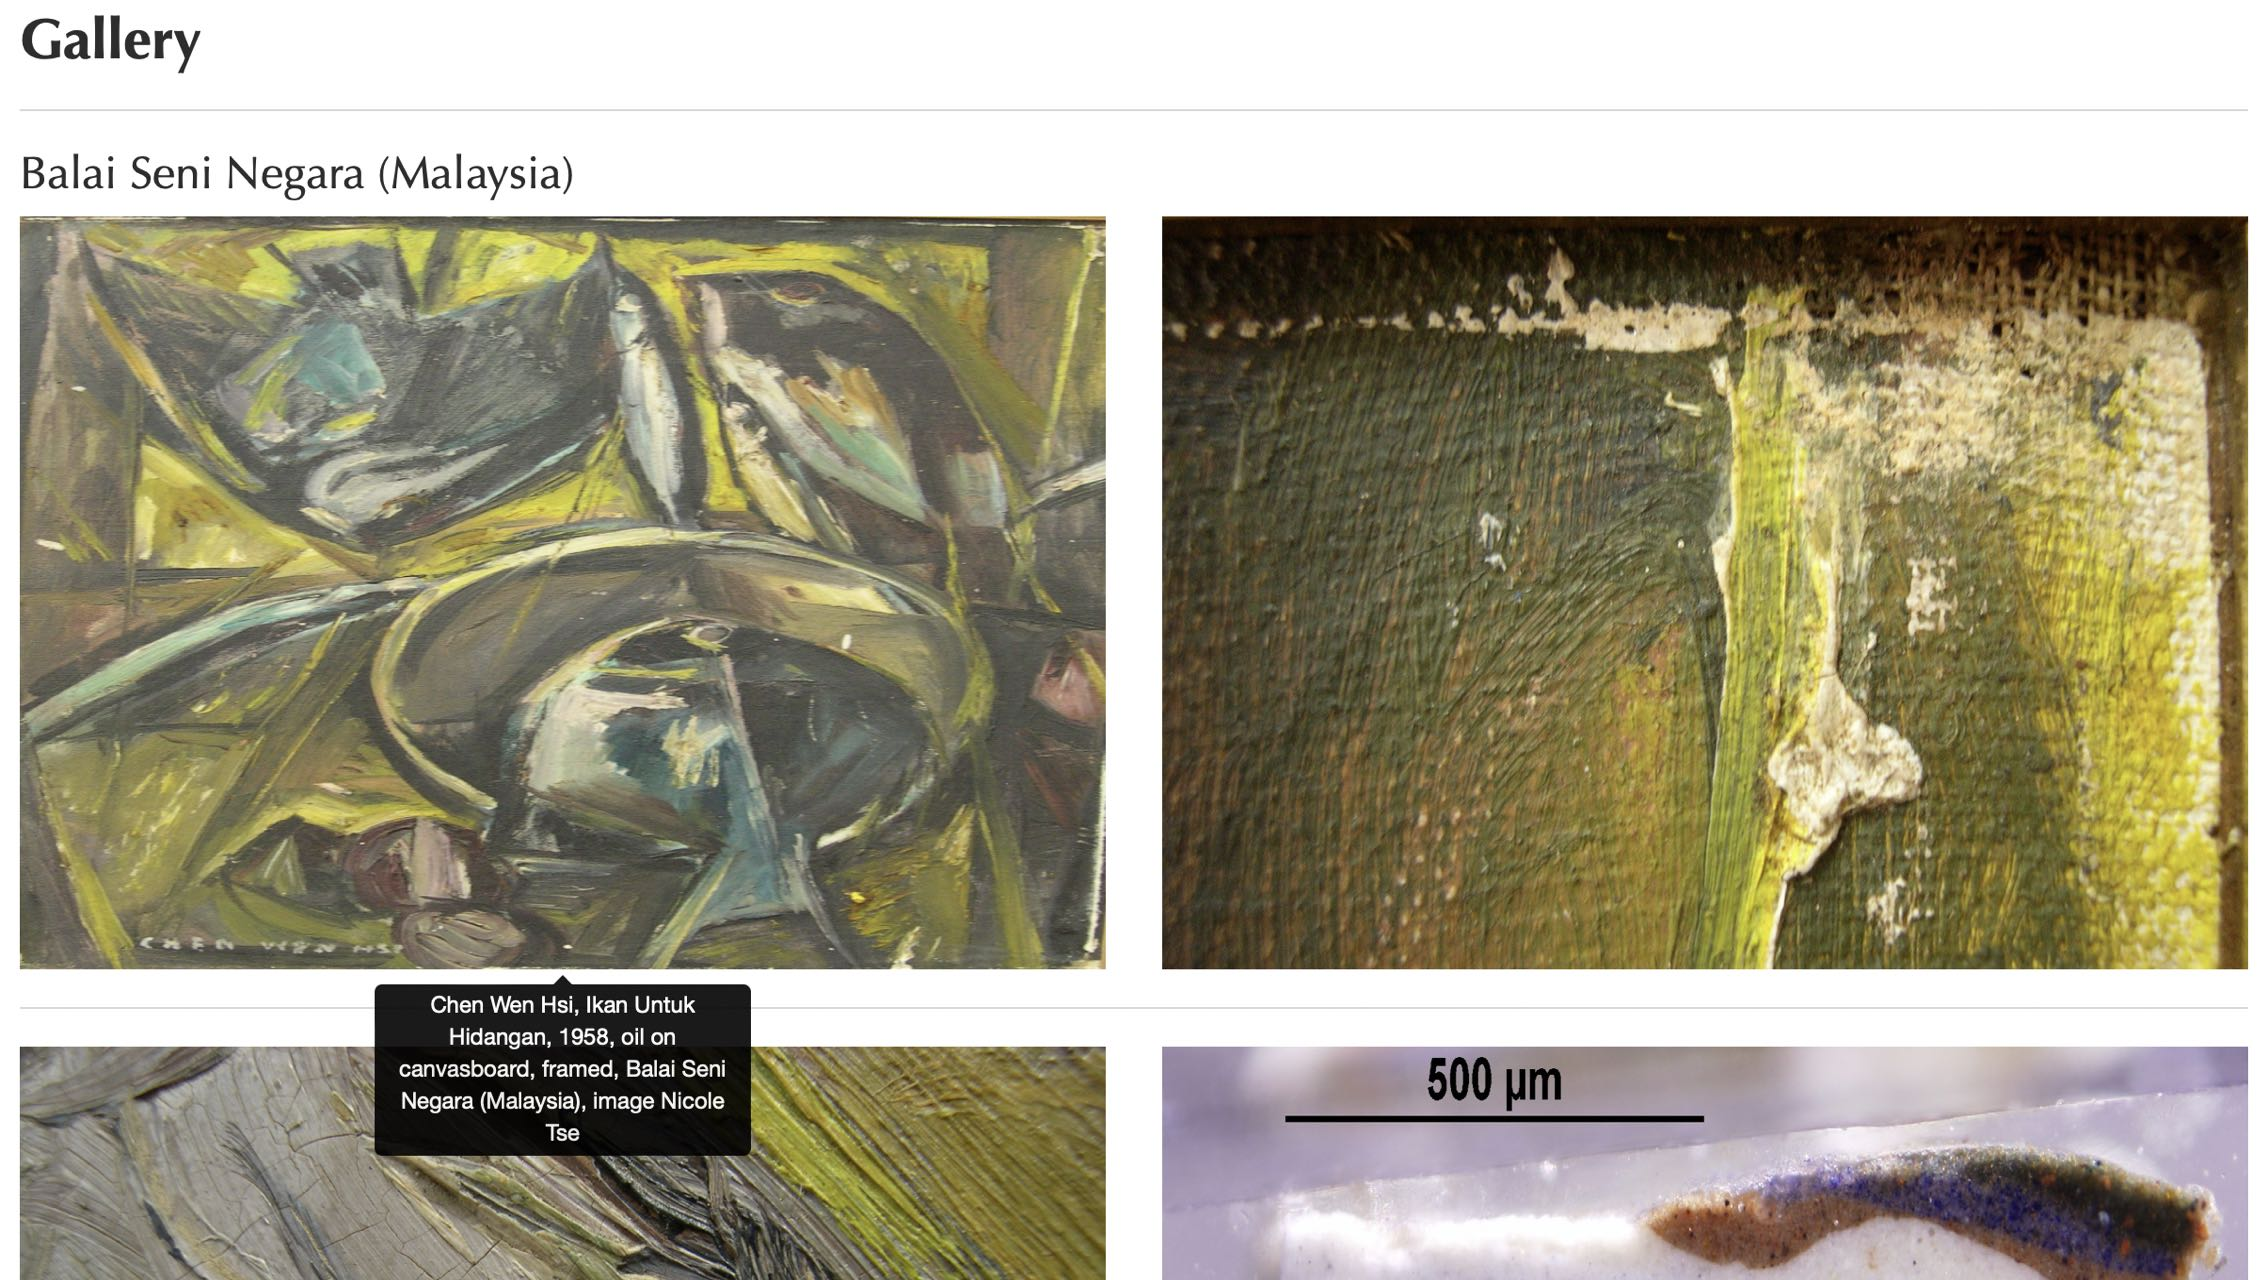
\includegraphics[scale=0.16]{images/gallery_tab.jpeg}
    \caption{Gallery Tab}
    \label{gallery_tab}
\end{figure}
The gallery tab is dedicated to showcasing the paintings that participated in the study. Six paintings from each museum were selected for the showcase by the client. As shown in Figure \ref{gallery_tab}, painting information is displayed via the tooltip when the user hovers above the image.

\subsubsection{The Dimension Tab}
\begin{figure}[H]
    \centering
    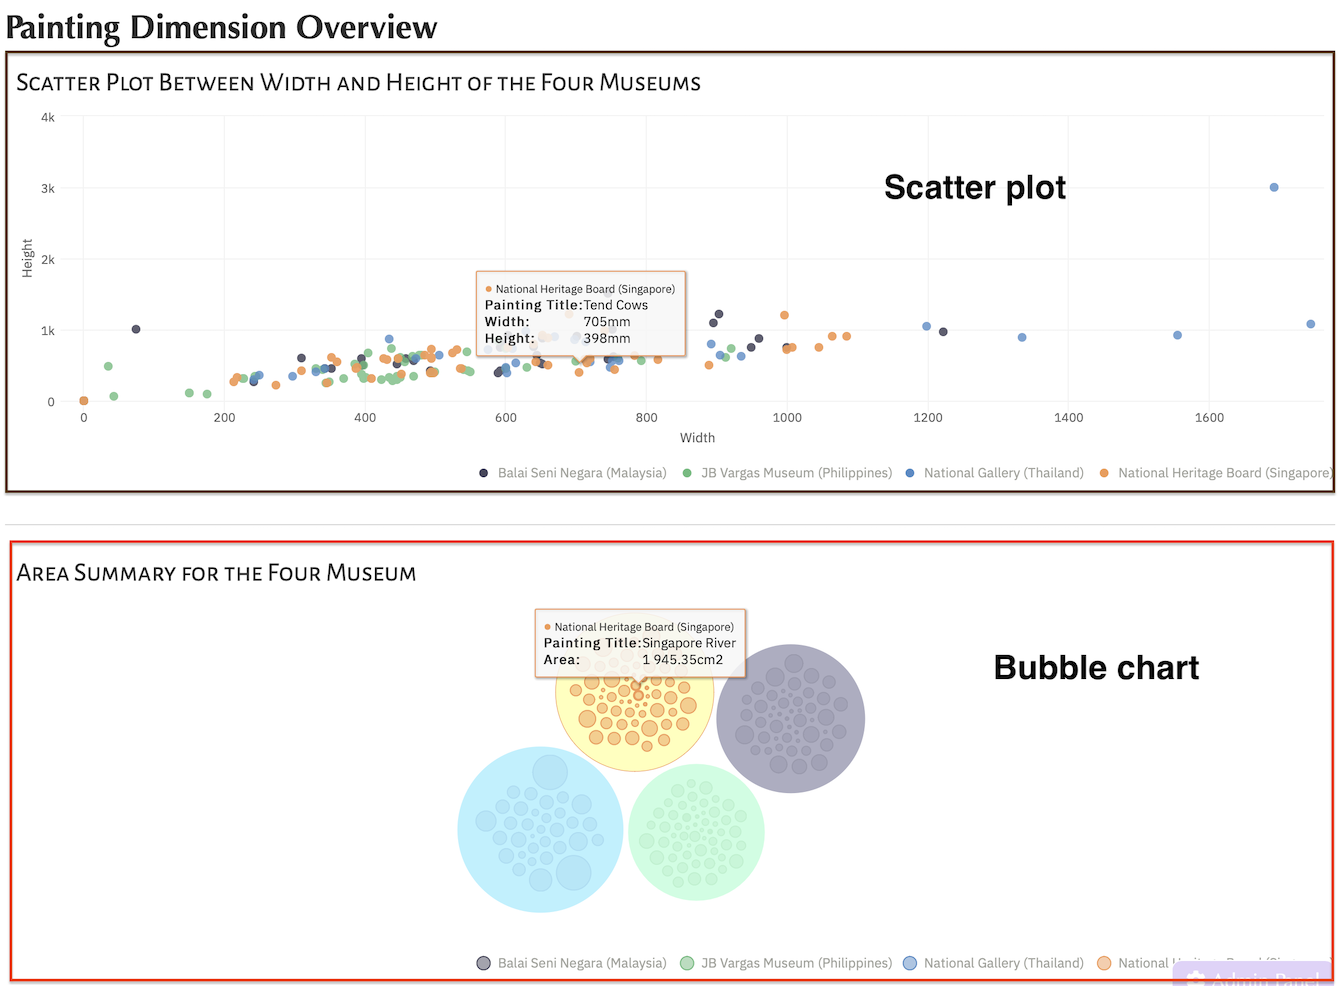
\includegraphics[scale=0.28]{images/dimension_screenshot.png}
    \caption{Dimension Tab}
    \label{dimension_tab}
\end{figure}

As shown in Figure \ref{dimension_tab}, this tab is created to give the user a clear picture of the dimension of the paintings from each collection. In the scatter plot shown above, we plotted the height against the width for each painting. Paintings from the different museums were separated by hue. Additionally, the tooltip will display information such as the painting's name, width, and height when the user hovers above the dots. Furthermore, the legend below the chart allows users to filter out museums that they do not wish to be included in the comparison.
\bigbreak
\noindent The packed bubble chart below serves the same purpose, but instead of comparing paintings using width and height, it directly shows the calculated area. Each painting was represented by a bubble, while the area of the painting determined the radius of the bubble. Furthermore, paintings were grouped by the museum, creating a visual hierarchy. Moreover, the tooltip displays general information about a painting: its name and calculated area, which provides a clear picture of the size of the paintings among the four museums.

\subsubsection{Tabs for the Painting Components}
\begin{figure}[H]
    \centering
    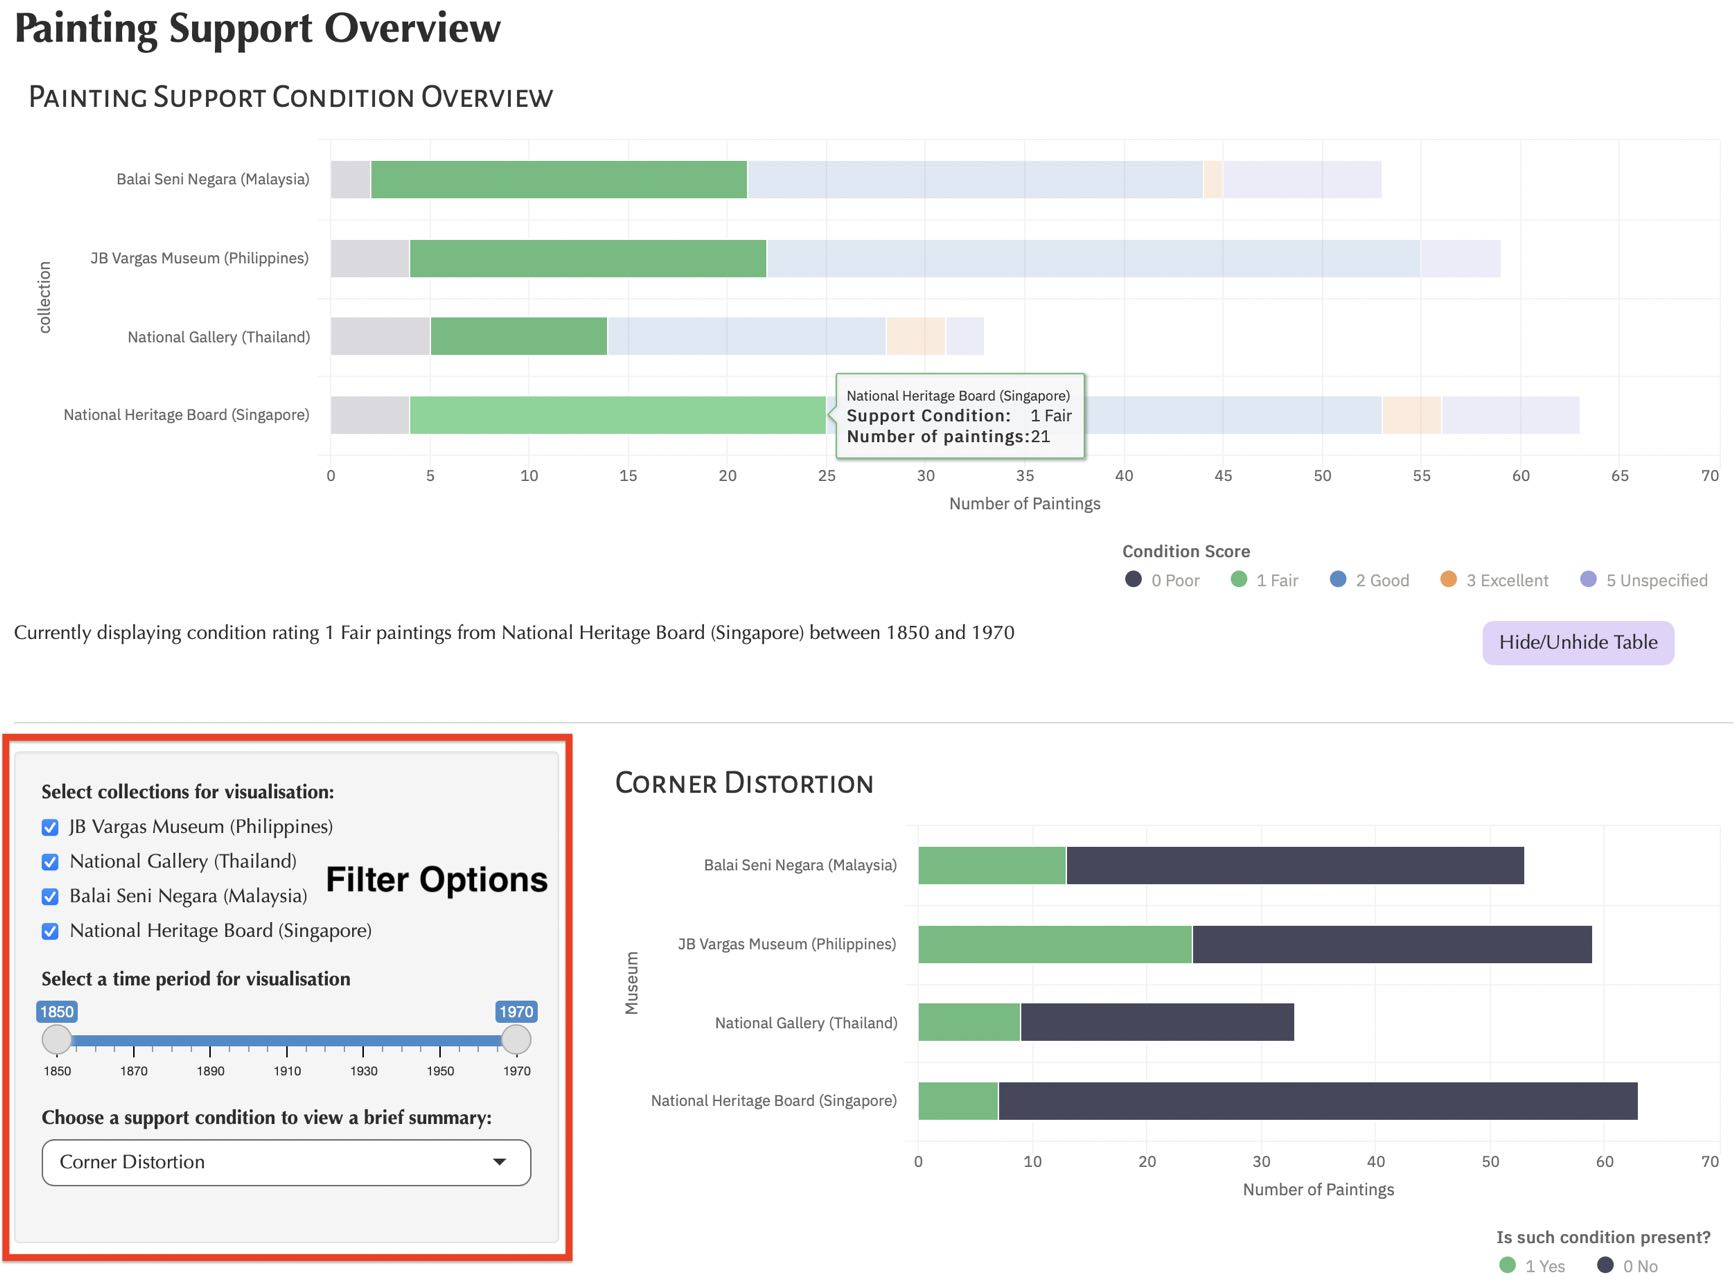
\includegraphics[scale=0.23]{images/ps_tab.jpeg}
    \caption{Painting Support Tab}
    \label{ps_tab}
\end{figure}

The interface of the painting support tab is shown in Figure \ref{ps_tab}. The design is shared among the tabs for the five components. The stacked bar chart above depicts the number of paintings in each museum, and each bar is further broken down into sub-amounts based on the component condition ratings. Moreover, the tooltip displays a brief summary of the hovering region: the condition and number of paintings belonging to the condition.
\bigbreak
\noindent Furthermore, the filter option shown in Figure \ref{filter} introduces interactivity, allowing the user to dynamically filter the museum to be included in the comparison, the period for visualisation, and the support condition for visualisation. Therefore, instead of laying charts for every support condition in the interface, the filter allows the user to choose which condition to visualise on the fly, keeping the interface tidy.
\begin{figure}[H]
    \centering
    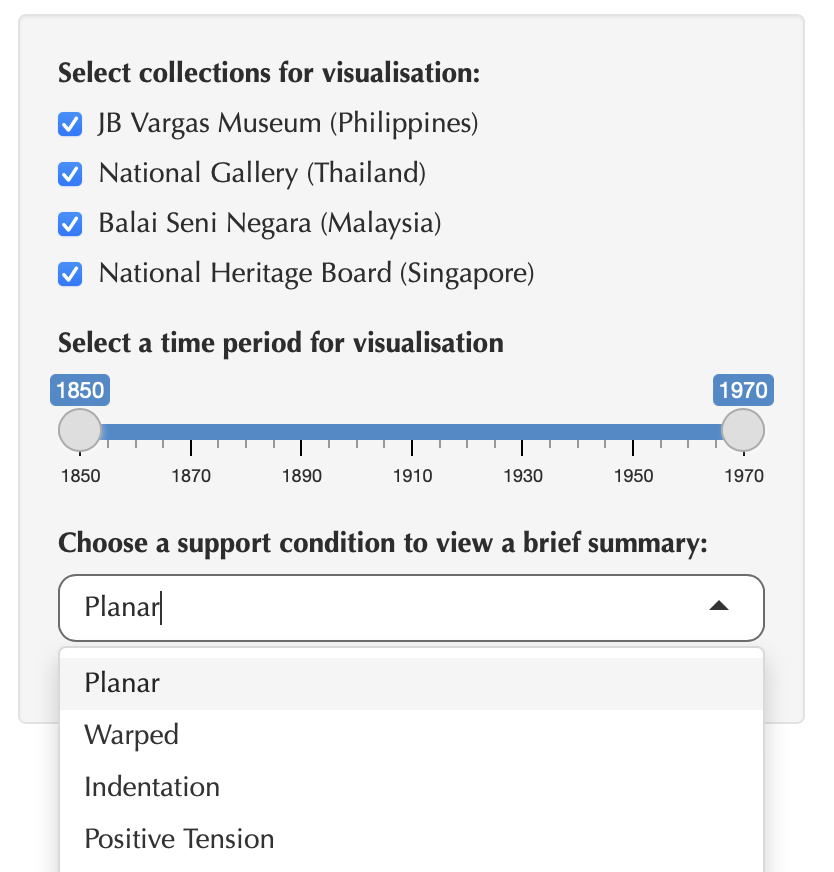
\includegraphics[scale=0.4]{images/filter_option.png}
    \caption{Filter Option}
    \label{filter}
\end{figure}

\subsubsection{The Dataset Exploration Tab}
\begin{figure}[H]
    \centering
    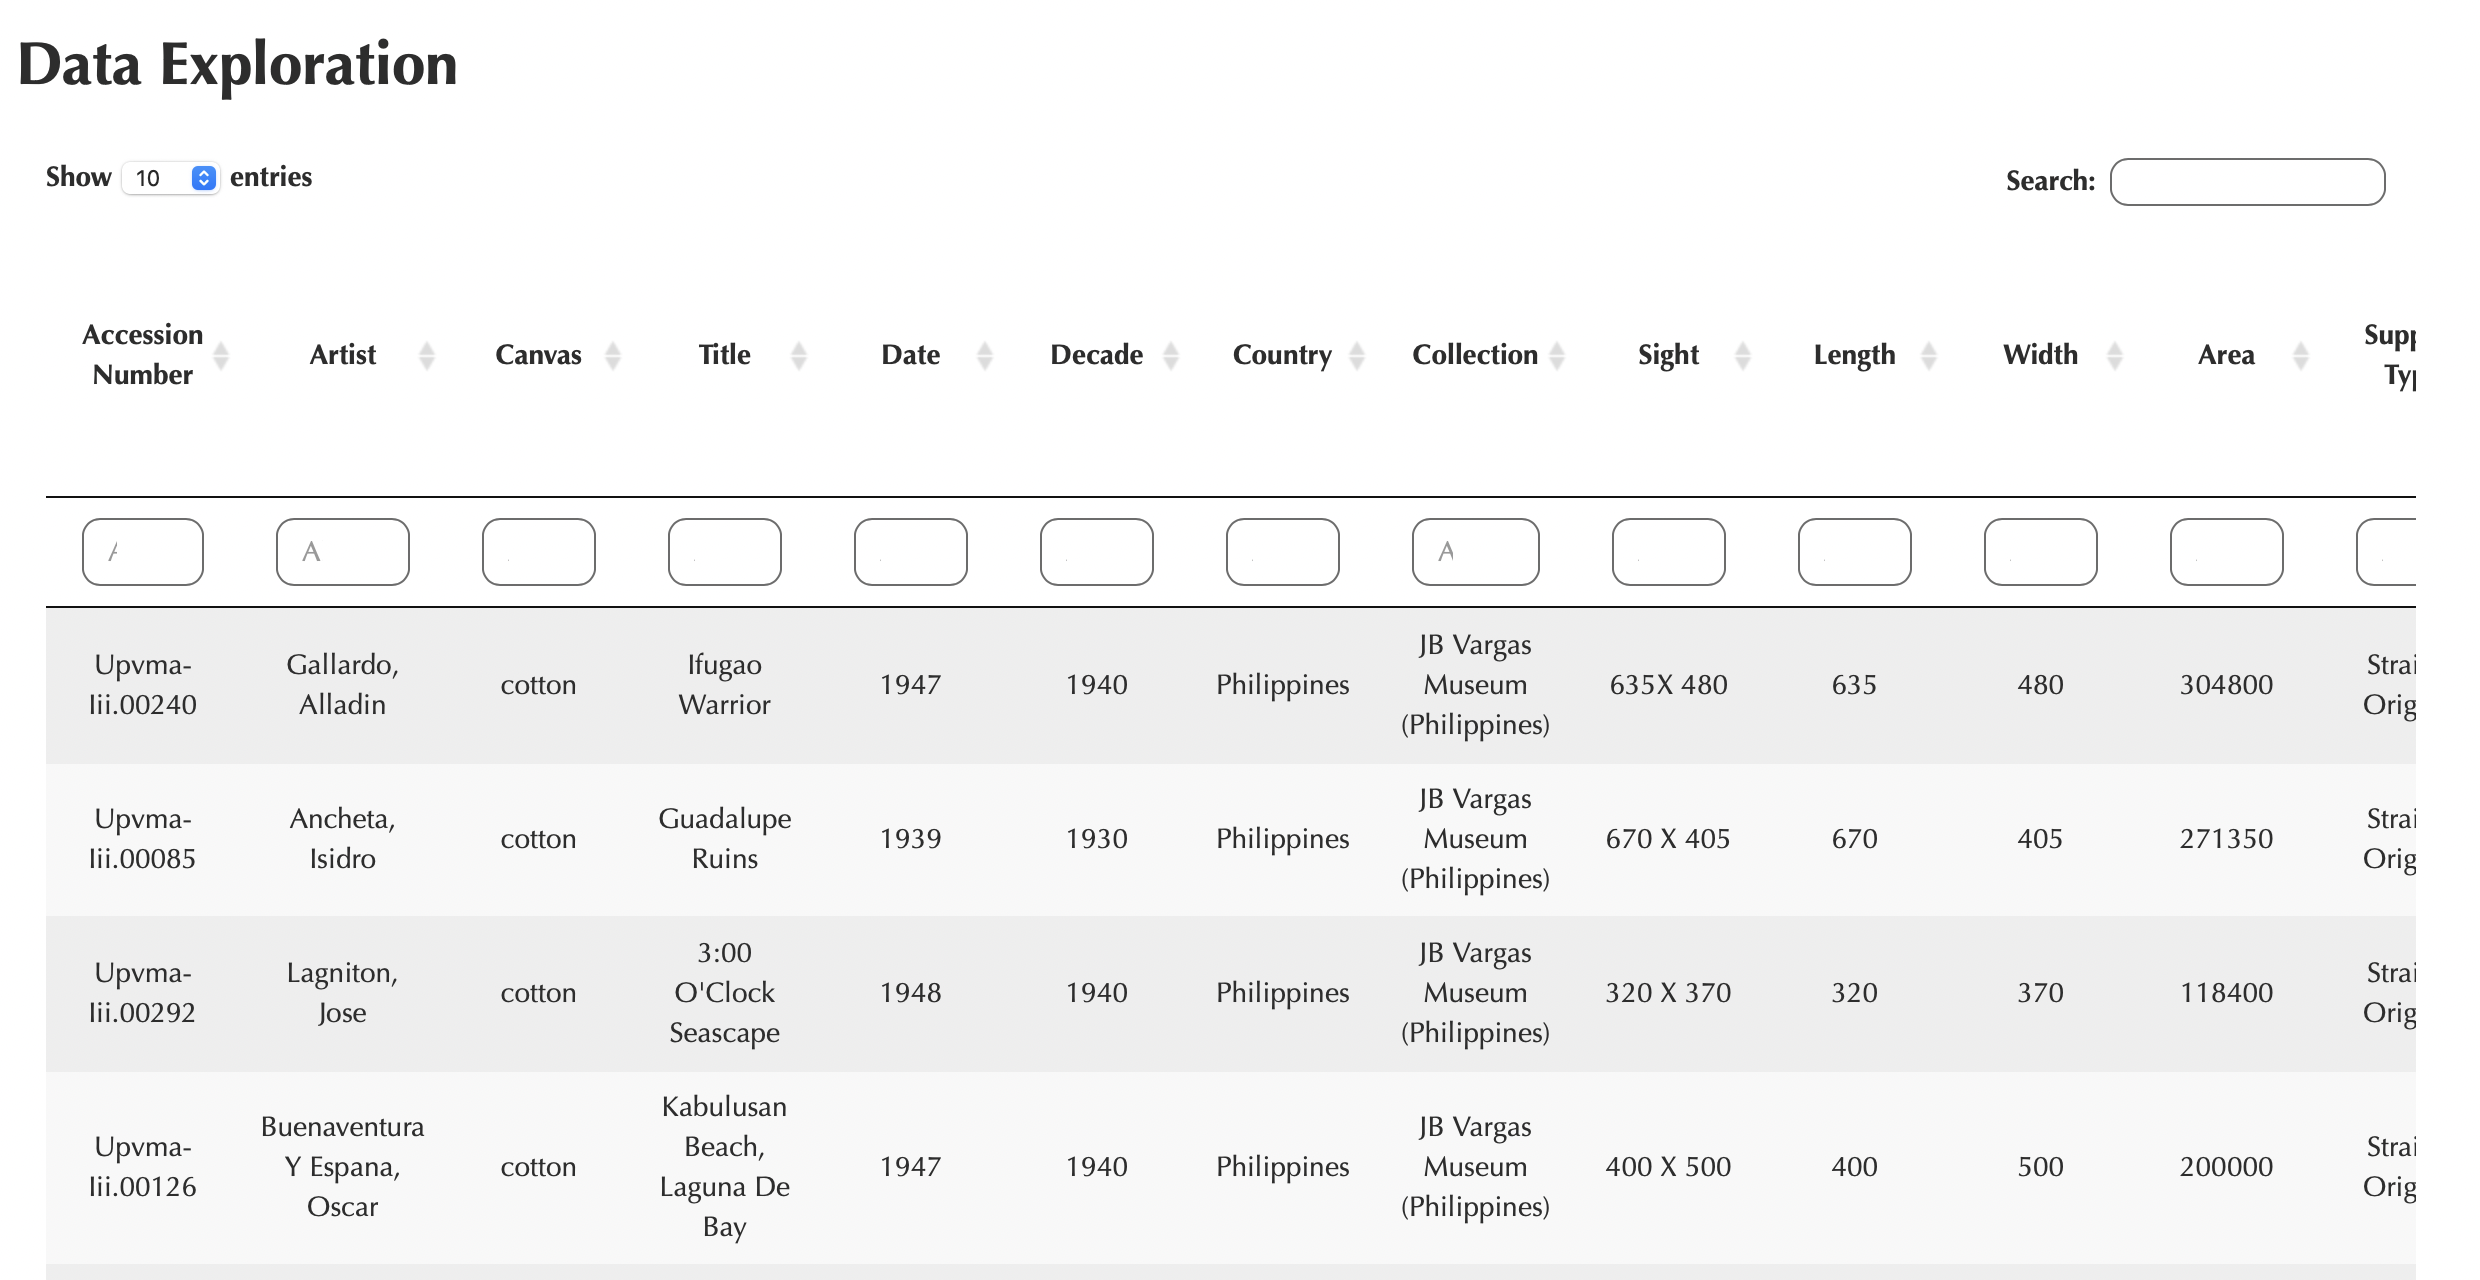
\includegraphics[scale=0.3]{images/explore_data.png}
    \caption{Explore Database Tab}
    \label{explore_tab}
\end{figure}
As shown in Figure \ref{explore_tab}, the data exploration tab was dedicated to dataset exploration. It allows the user to browse a cleaned version of the dataset within the dashboard. In addition, a filter and search option have been added for each attribute, allowing the user to locate specific content by inputting a search string or selecting filter options.

\subsubsection{Reactivity and Click Event}
The main problem we encountered while building the dashboard was that basic interactive visualisation only provides limited information through the popup labels, such as the number of paintings under a specific condition. As a result, it loses a lot of information because it only tells the user how many paintings were under a particular condition, but it does not tell the user what paintings are actually under those conditions. Therefore, our proposed solution to this problem is to use the reactive functionality of Shiny and Highcharter's ability to capture the user's click events.
\begin{figure}[H]
    \centering
    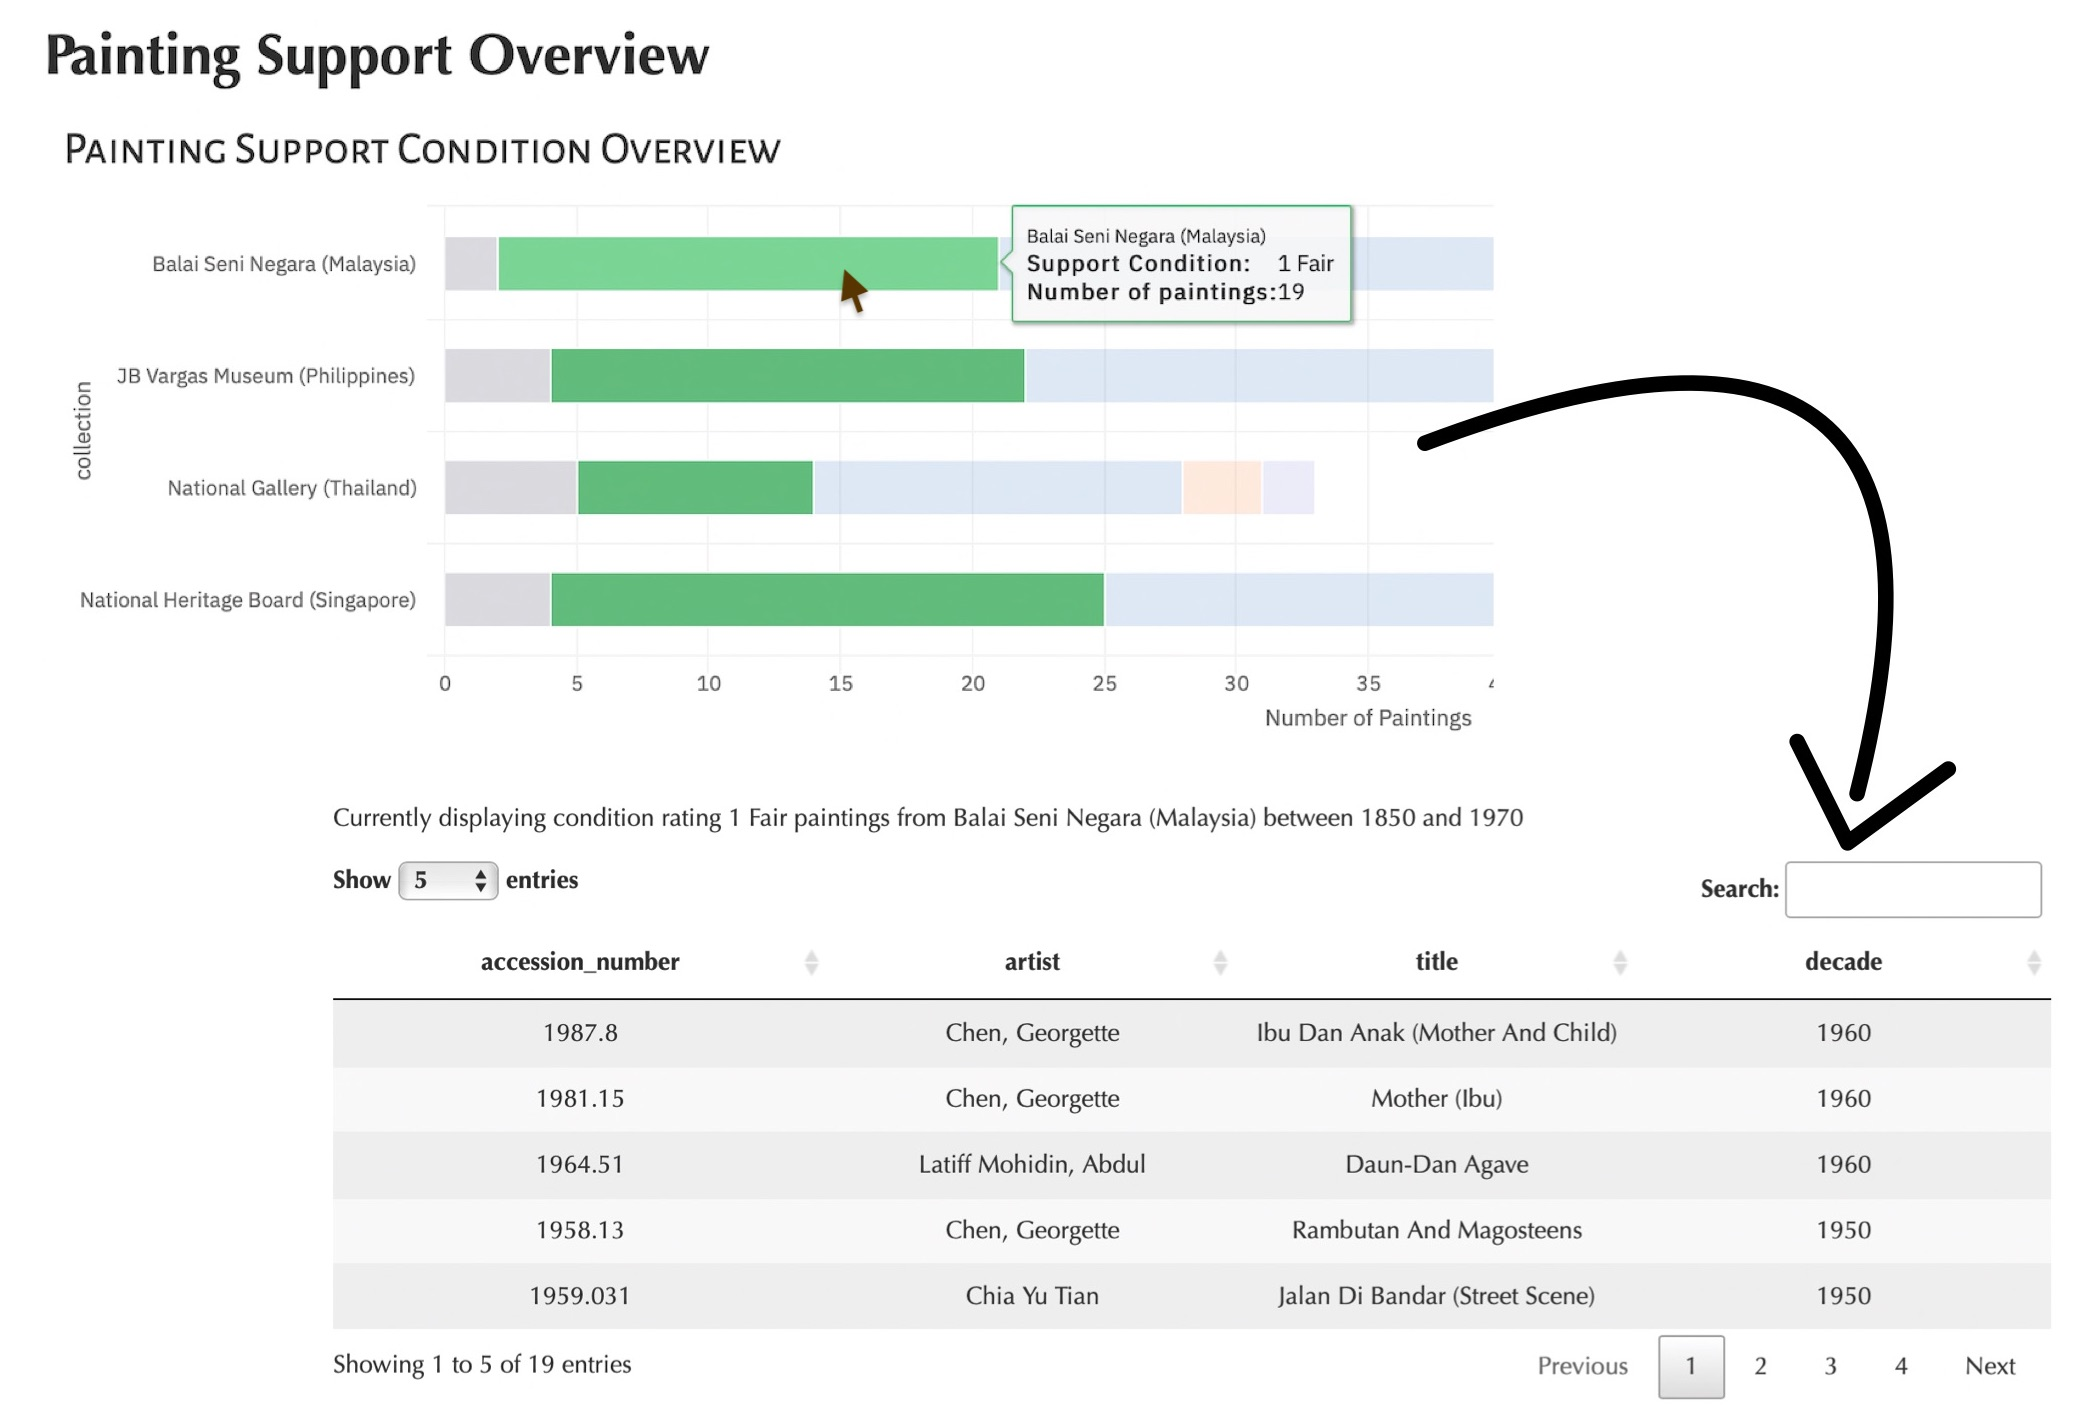
\includegraphics[scale=0.2]{images/click_event.jpeg}
    \caption{Click Event Example}
    \label{click_event}
\end{figure}
\noindent An illustration of our approach to this problem is shown in Figure \ref{click_event}. Typically, when the mouse hovers above a specific section of the interactive plot, a tooltip will pop up and display some information about the selected part. However, with the introduction of reactivity and click events, information on the hovered section will be recorded when the user clicks on the hovered section. This effectively allows the dashboard application to filter the dataset and produce a summary table below the plot that contains all the paintings corresponding to the conditions of the selected section. Therefore, adding this functionality to our dashboard allows us to create visualisation without sacrificing the information of the original dataset. It also effectively groups paintings that belong to a given category, allowing users to query the data based on painting conditions.

\subsubsection{Polished for Authentication}
To ensure the confidentiality of the dashboard, we have utilised the polished package. The login page, as shown in Figure \ref{Login_Homepage}, was created by using the Polished package, which allows us to customise the colour styling and add logos on login page.

\begin{figure}[H]
    \centering
    
\includegraphics[scale=0.26]{images/Polished_login.png}
    \caption{Login page}
    \label{Login_Homepage}
\end{figure}

\begin{figure}[H]
    \centering
    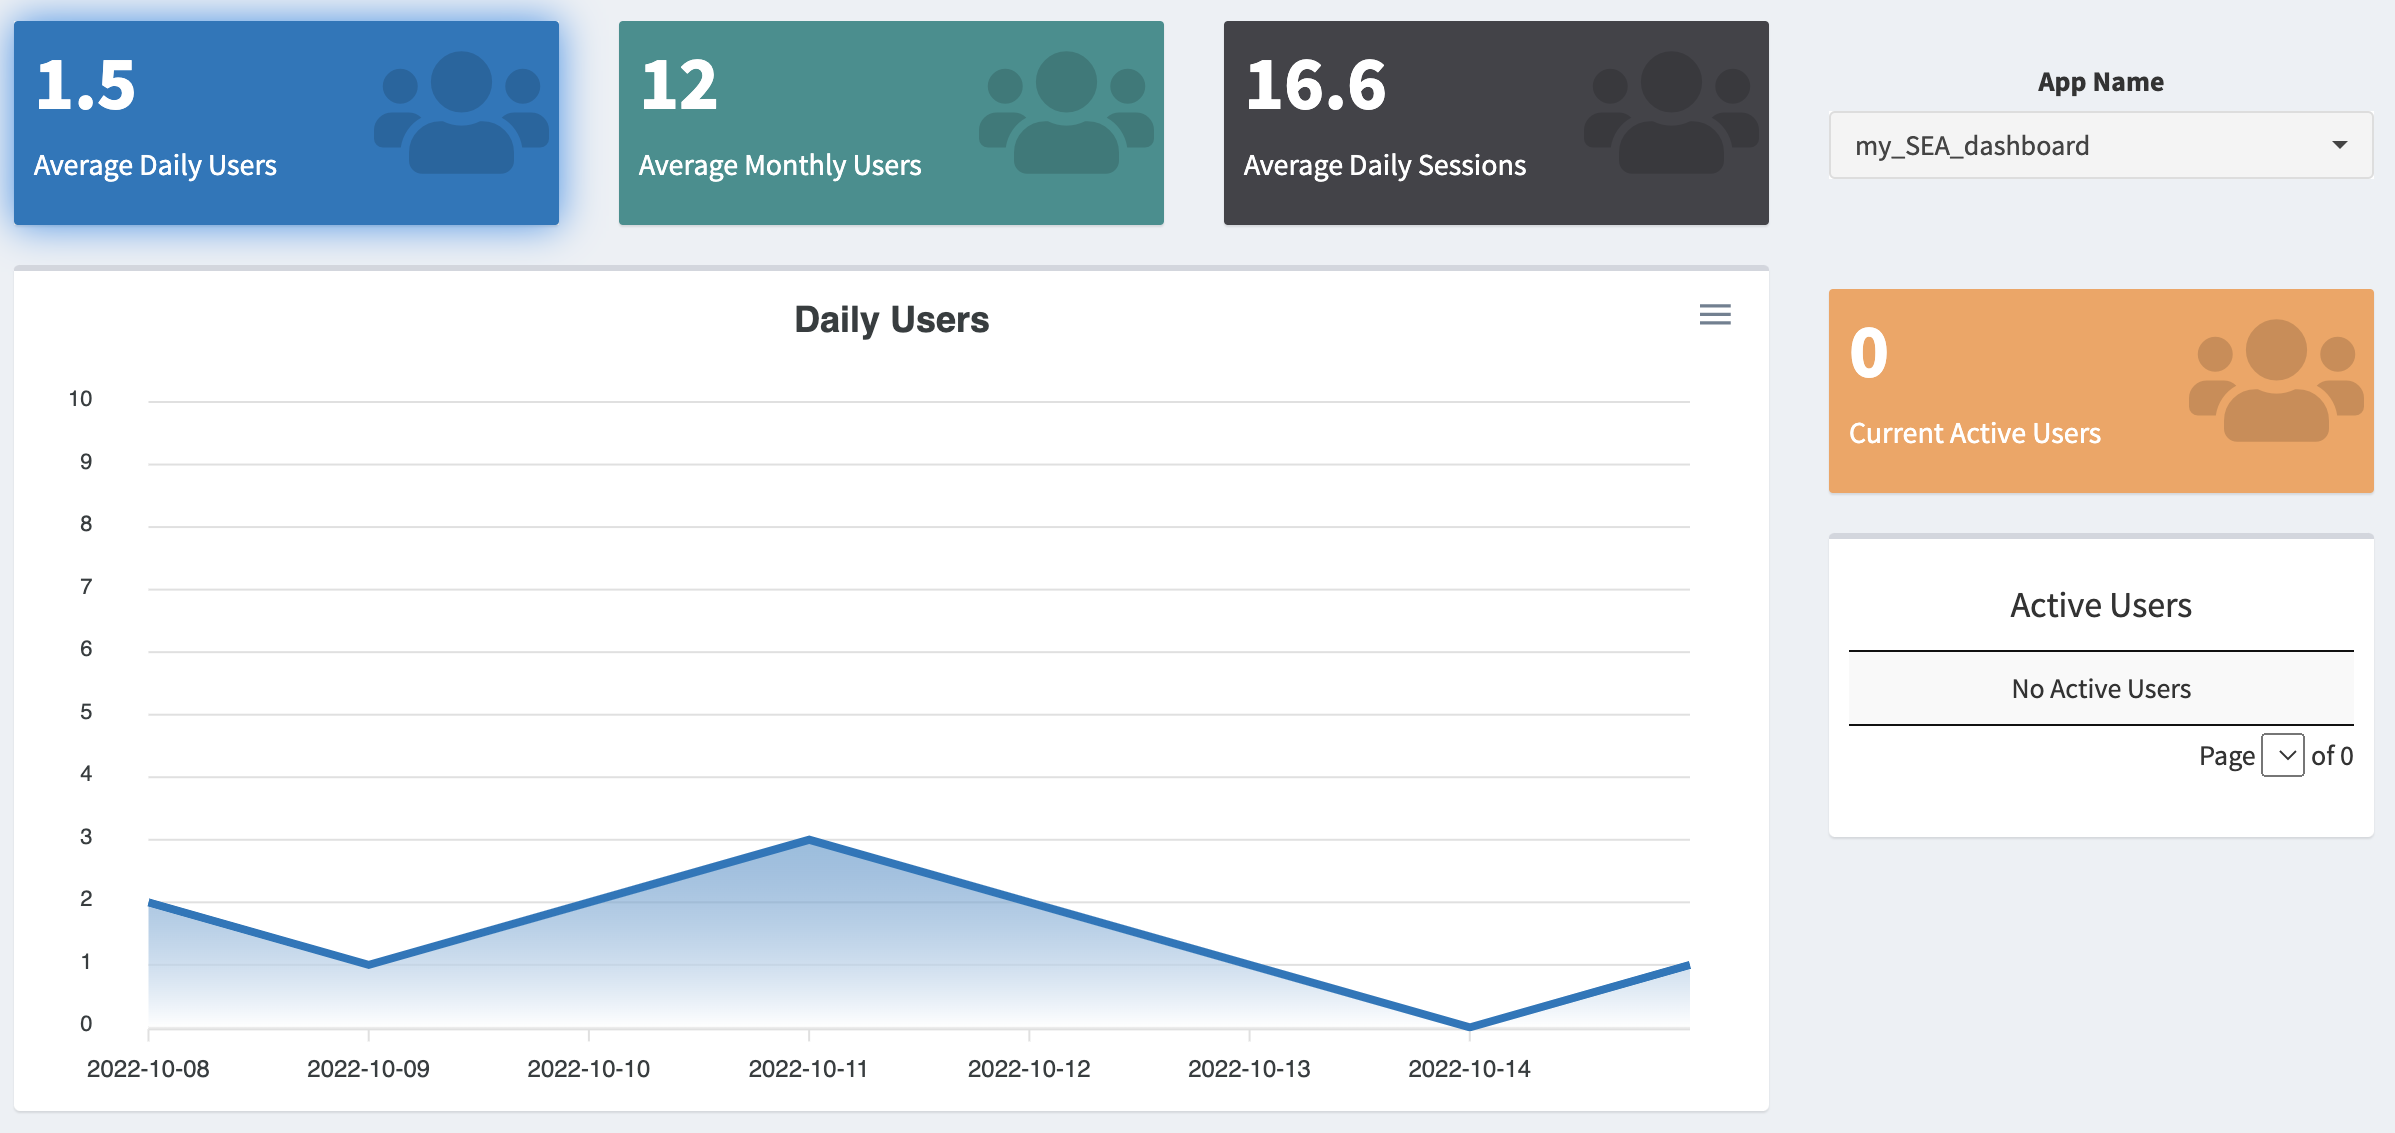
\includegraphics[scale=0.35]{images/Polished_1.png}
    \caption{Polished Usage Monitor}
    \label{Polished_dashboard}
\end{figure}

\noindent Furthermore, the polished package also comes with an easy-to-use dashboard website to monitor users' usage as shown in Figure \ref{Polished_dashboard}. This site has functionality allowing admin users to maintain user roles and authorisation of the application, as exhibited in Figure \ref{Polished_dashboard_2}.

\begin{figure}[H]
    \centering
    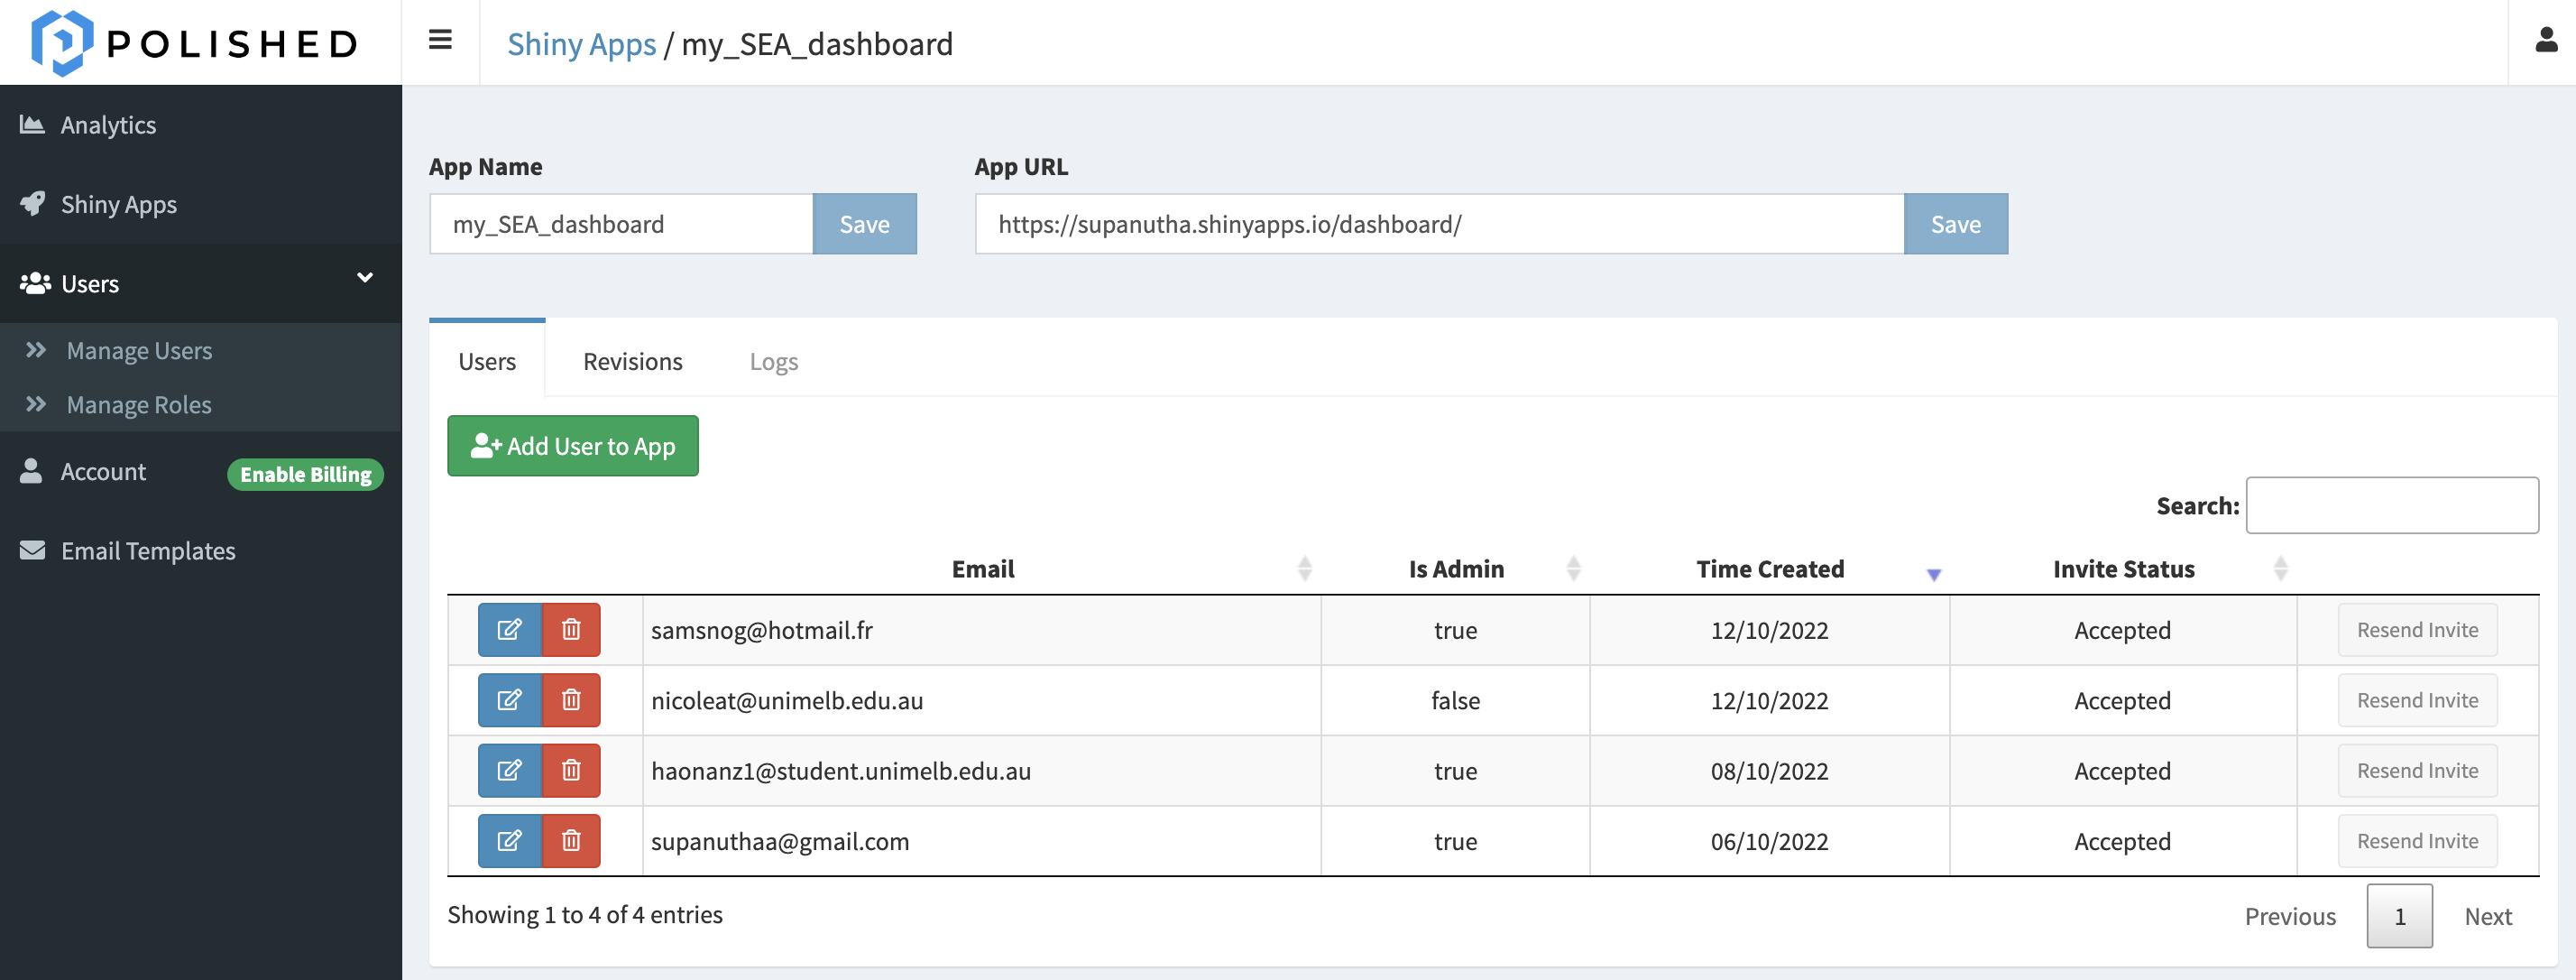
\includegraphics[scale=0.3]{images/Polished_2.png}
    \caption{Polished User Management}
    \label{Polished_dashboard_2}
\end{figure}

\subsection{Section Summary}
In this section, we have mainly presented our approach and a summary of the constructed dashboard. Along the way, some challenges arose, but solutions were found. As an achievement, the client has shared the dashboard with museums involved in the study behind this project, and we have received beneficial feedback that is useful future improvements of the dashboard.

\section{Independence Testing and Relationship Visualisation}
As discussed in the data preprocessing section, given that all the painting condition attributes in the dataset are mostly categorical; therefore, it is impossible to run correlation analysis to identify the relationship between two selected categorical variables since, by definition, they cannot yield a mean, and we cannot compute the covariance between two categorical variables. For that reason, we've mainly applied three methods to test the relationship between the attributes.

\subsection{Contingency Table Analysis with $\chi^2$ Test of Independence and Log-linear Model}
One method for dealing with categorical data is Log-linear model and $\chi^2$ test of independence, which is a hypothesis testing method that is used to check whether the two categorical variables are associated or not. As with all other hypothesis testing, we've defined the null ($\mathtt{H_0}$) and alternative ($\mathtt{H_1}$) hypothesis as,
\begin{itemize}
    \item $\mathtt{H_0}$: There is no association between the two categorical variables
    \item $\mathtt{H_1}$: There is association between the two categorical variables
\end{itemize}

\noindent We will first introduce the concept of test statistics and \textit{p-value}. Test statistics measures the degree of agreement between a sample of data and the null hypothesis, while \textit{p-value} tells us how likely the test statistics could have occurred under the null hypothesis. The general testing rule is if the test statistics are higher than the critical value, or the p-value is less than the significance level of 0.05. We would reject the null hypothesis and prefer the alternative.

\begin{table}[H]
\begin{center}
\begin{tabular}{lrrr}
\hline
& Indentation (No) & Indentation (Yes) & Total \\
\hline
Holes (No) & 142 & 20 & 162 \\
Holes (Yes) & 30 & 16 &  46 \\
\hline
Total & 172 & 36 & 208 \\
\hline
\end{tabular}
\end{center}
\caption{Contingency Table of Indentation vs Holes (Observed)}
\label{indent-holes}
\end{table}

\noindent To formulate the $\chi^2$ test, we summarise the two selected categorical variables as a contingency table, an example was given in Table \ref{indent-holes}. Cells of the table represents the observation frequency fallen into the given combination. The test itself works by comparing the observation frequencies to the calculated expected frequencies under the null hypothesis using Pearson's $\chi^2$ statistics, where the expected frequency of a cell and $\chi^2$ test statistic is calculated as followed,
\begin{equation*}
    Expected_k = \frac{\text{Column Total} \times \text{Row Total}}{\text{Table Total}} \quad\text{and}\quad
    \hat{\chi}^2=\sum_{k=1}^{n} \frac{(Observed_k - Expected_k)^2}{Expected_k}
\end{equation*}
If the corresponding \textit{p-value} of $\hat{\chi}^2$ is less than the significance level of 0.05. In which the difference between the observed and expected distributions is statistically significant. We would then have sufficient evidence to reject the null hypothesis, claim the two variables are associated and vice versa. The test statistics $\hat{\chi}^2$ could also be approximated by using the residual deviance obtained from the Log-linear model, which effectively allows us to perform the test using more than two categorical variables.

\subsection{Fisher's Exact Test}
The problem with $\chi^2$ test is that, for a reliable test, we need a large balanced dataset and the expected frequency of cells in the contingency table are required to be at least 5 \cite{mcdonald}. But due to the size of the dataset, this assumption could not be satisfied.
\bigbreak
\noindent An alternative method is to use the Fisher's exact test, where the test procedure are similar to the $\chi^2$ test, comparing the \textit{p-value} against the significance level. It is more effective than the $\chi^2$ test when the expected frequencies and the dataset are small as suggested by related work, since Fisher's exact test does not rely on an approximation of the test statistics that becomes exact when the data size approaches infinity, instead it directly assesses the null distribution by calculating the probability of getting the observed data using the hypergeometric distribution \cite{mcdonald}.

\subsection{Mosaic Plot}
Furthermore, we have used mosaic plot to visualise the relationship between two related categorical attributes. Mosaic plot is an effective way to visualise contingency tables. The general idea is to represent each cell of the table with a box, where the corresponding cell counts determine the size of the box. The height of each box is the proportion of individuals in the column which fall into that cell, while the width is the same for all boxes of the same column and is equal to the total count in that column. As an example, the mosaic plot for Table \ref{indent-holes} is shown in Figure \ref{mosaic_example}.

\begin{figure}[H]
    \centering
    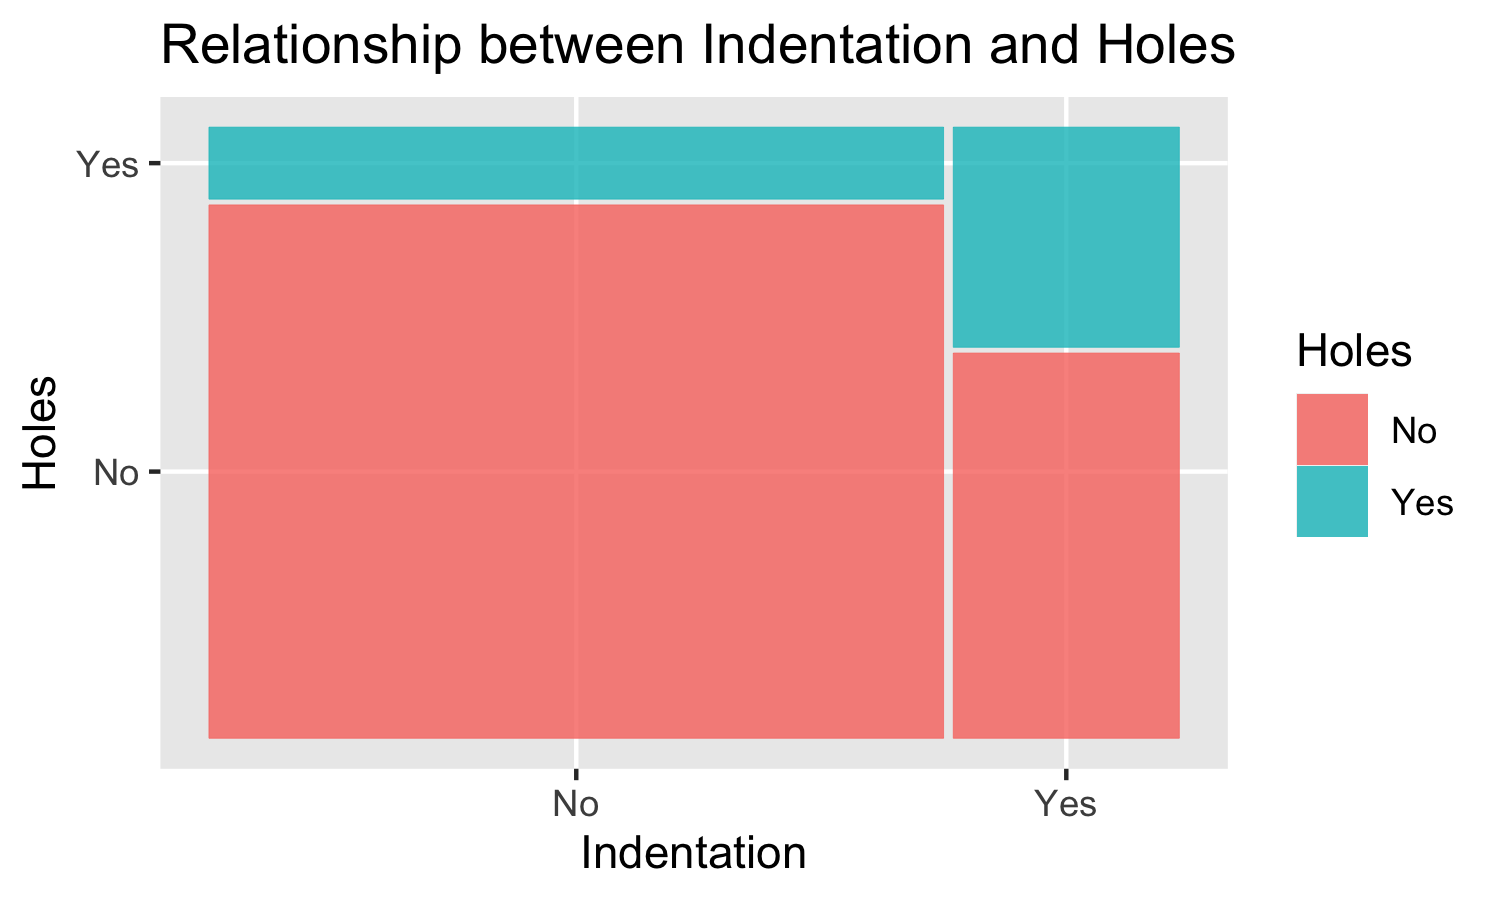
\includegraphics[scale=0.2]{images/indent_holes_sample.png}
    \caption{Example Mosaic Plot of Holes vs. Indentation}
    \label{mosaic_example}
\end{figure}

\subsection{Limitation of the Test}
During the exploratory data analysis, we noticed that some paintings were not assigned with a condition ratings. Therefore, paintings without an condition ratings on paint support, ground layer, and paint layer will be excluded from testing.
\bigbreak
\noindent Furthermore, given paintings were sourced from four different museums, thus we would like to test the condition independence of each attributes given different museums. To do this, we've fitted the log-linear model for each combination of the categorical variables, and performed $\chi^2$ test to determine whether the are likely to be related or not given different museum. The fitted log-linear model is given below, where $\mathtt{M}$, $\mathtt{C1}$, and $\mathtt{C2}$ is the museum, first condition attribute, second condition attribute, respectively. And $\lambda_{ijk}$ is the cell observed frequency of the contingency table.
\[log(\lambda_{ijk}) = \mu + \mathtt{M_i} + \mathtt{C1_j} + \mathtt{C2_k} + (\mathtt{M}\cdot\mathtt{C1})_{ij} + (\mathtt{M}\cdot\mathtt{C2})_{ik}\]
However, due to the sparse nature and the small size of the dataset, zero cells have been a significant issue when constructing the table and fitting the model. Zero cells in the contingency table can be distinguished as sampling zeros and structural zeros. The former is due to sampling variability, and the latter are cells known to have zero values. Thus, in our case, the zeros can be treated as structural zeros, given that the cell values are simply missing because it has no paintings from the sample population that fit into the category. 
\bigbreak
\noindent One solution will be testing quasi-independence, where zero cells will be excluded from analysis when testing independence. However, when the table was overcrowded with zero cells, there was not enough data to provide a trustworthy model fit and test result, where the model will be saturated as the residual deviance and degrees of freedom were reduced to zeros, causing overfitting. Therefore, the results discussed only considers the painting collection as a whole, without the interaction of museums. Last but not least, it is important to note that the test of independence only tells whether two attributes are related to one another, and it does not necessarily imply any causal effect of a variable to another.

\subsection{Testing Algorithm Description}
We have implemented an algorithm for testing pairwise independence between the attributes of each layer, utilising the hypothesis testing function of R. The algorithms starts with the first attribute $v_1$ of the input dataframe that consists of $k$ attributes to be tested, then it's relationship with the other $k-1$ attributes of the dataframe were then tested using Fisher's Exact test. 
\bigbreak
\noindent The obtained \textit{p-value} of each test were then used to assess the two attribute's relationship. If the \textit{p-value} is less than the significance level 0.05, we will reject the null hypothesis and conclude that the two are associated, vice versa. We repeat the steps above until each combination is tested. The pseudo-code of our algorithm is shown in Algorithm \ref{alg}.
\bigbreak
\begin{algorithm}[H]
\SetAlgoLined
\KwInput{Data frame consists of testing attributes}
\KwOutput{Data frame consists of testing results}
 $\textit{attributes}\gets colNames(\textbf{Input})$\;
 \For{$v_i\:\:in\:\:attributes$}{
  \For{$v_j\:\:in\:\:attributes$} {
  \eIf{$v_i=v_j$}{
   do nothing\;
   }{
   $table \gets$ ftable($v_i,\:v_j$)\;
   $\textit{p-value} \gets$ fisher.test($table$)\;
   \eIf{$\textit{p-value} < 0.05$}{
   $v_i$ and $v_j$ is associated\;
   } {
   $v_i$ and $v_j$ is independent\;
   }
  }
  }
 }
 \caption{Independence testing for pairwise attributes}
 \label{alg}
\end{algorithm}

\subsection{Result and Visualising Relationships}
\subsubsection{Relationship Between Paint Support, Ground Layer and Paint Layer Ratings}
Firstly, we have tested the association between the paint support, ground layer and paint layer condition ratings. As mentioned in the introduction, these three components were stacked on top of each other in a painting. Therefore, we are interested to see if these conditions are closely related with each other.
\begin{table}[H]
\begin{center}
\begin{tabular}{llr}
\hline
 Attribute 1 & Attribute 2 & \textit{p-value} \\
\hline
Paint Support Condition & Ground Condition  & 2.907e-06  \\
\hline
Paint Support Condition & Paint Layer Condition & 2.661e-06  \\
\hline
Ground Condition & Paint Layer Condition & 5.658e-06  \\
\hline
\end{tabular}
\end{center}
\caption{Fisher's Exact Test Result of the Three Condition Ratings}
\label{three-cond}
\end{table}
\noindent As we can see from the result table \ref{three-cond} above, the low p-values suggest the three condition ratings were highly associated with each other. The mosaic plot shown in Figure \ref{ps_pl_mosaic} depicts the relationship between paint support condition ratings and paint layer condition ratings, we can see a clear trend between the two condition ratings, the proportion of paintings having good and excellent ground layer condition rating increases as the paint support condition rating increases from poor to excellent. While the proportion of paintings with poor and fair ground layer condition rating gradually declines as paint support condition rating increases.

\begin{figure}[H]
    \centering
    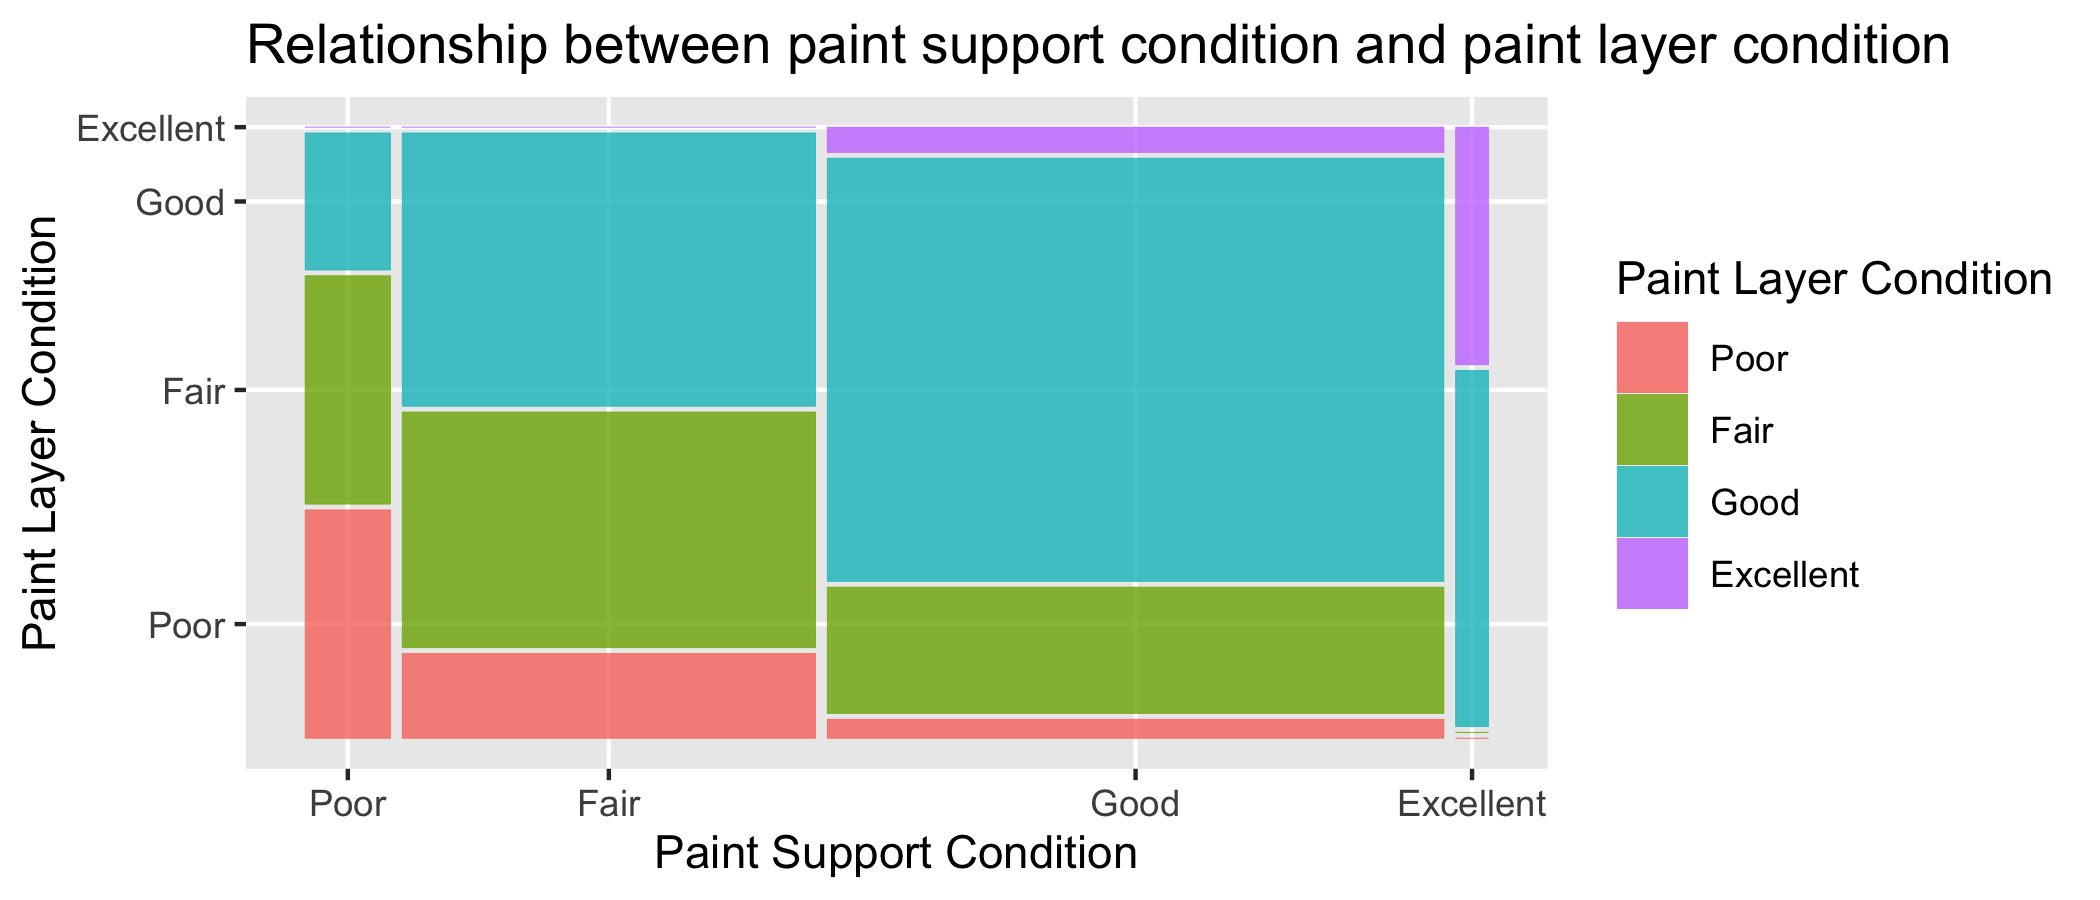
\includegraphics[scale=0.19]{images/ps_pl_mosaic.png}
    \caption{Relationship Between Paint Support Condition and Paint Layer Condition}
    \label{ps_pl_mosaic}
\end{figure}

\noindent It is no surprise that a similar trend could also be seen with the other two combination, as shown in Figure \ref{ps_gr_mosaic} and Figure \ref{gr_pl_mosaic}.

\begin{figure}[H]
    \centering
    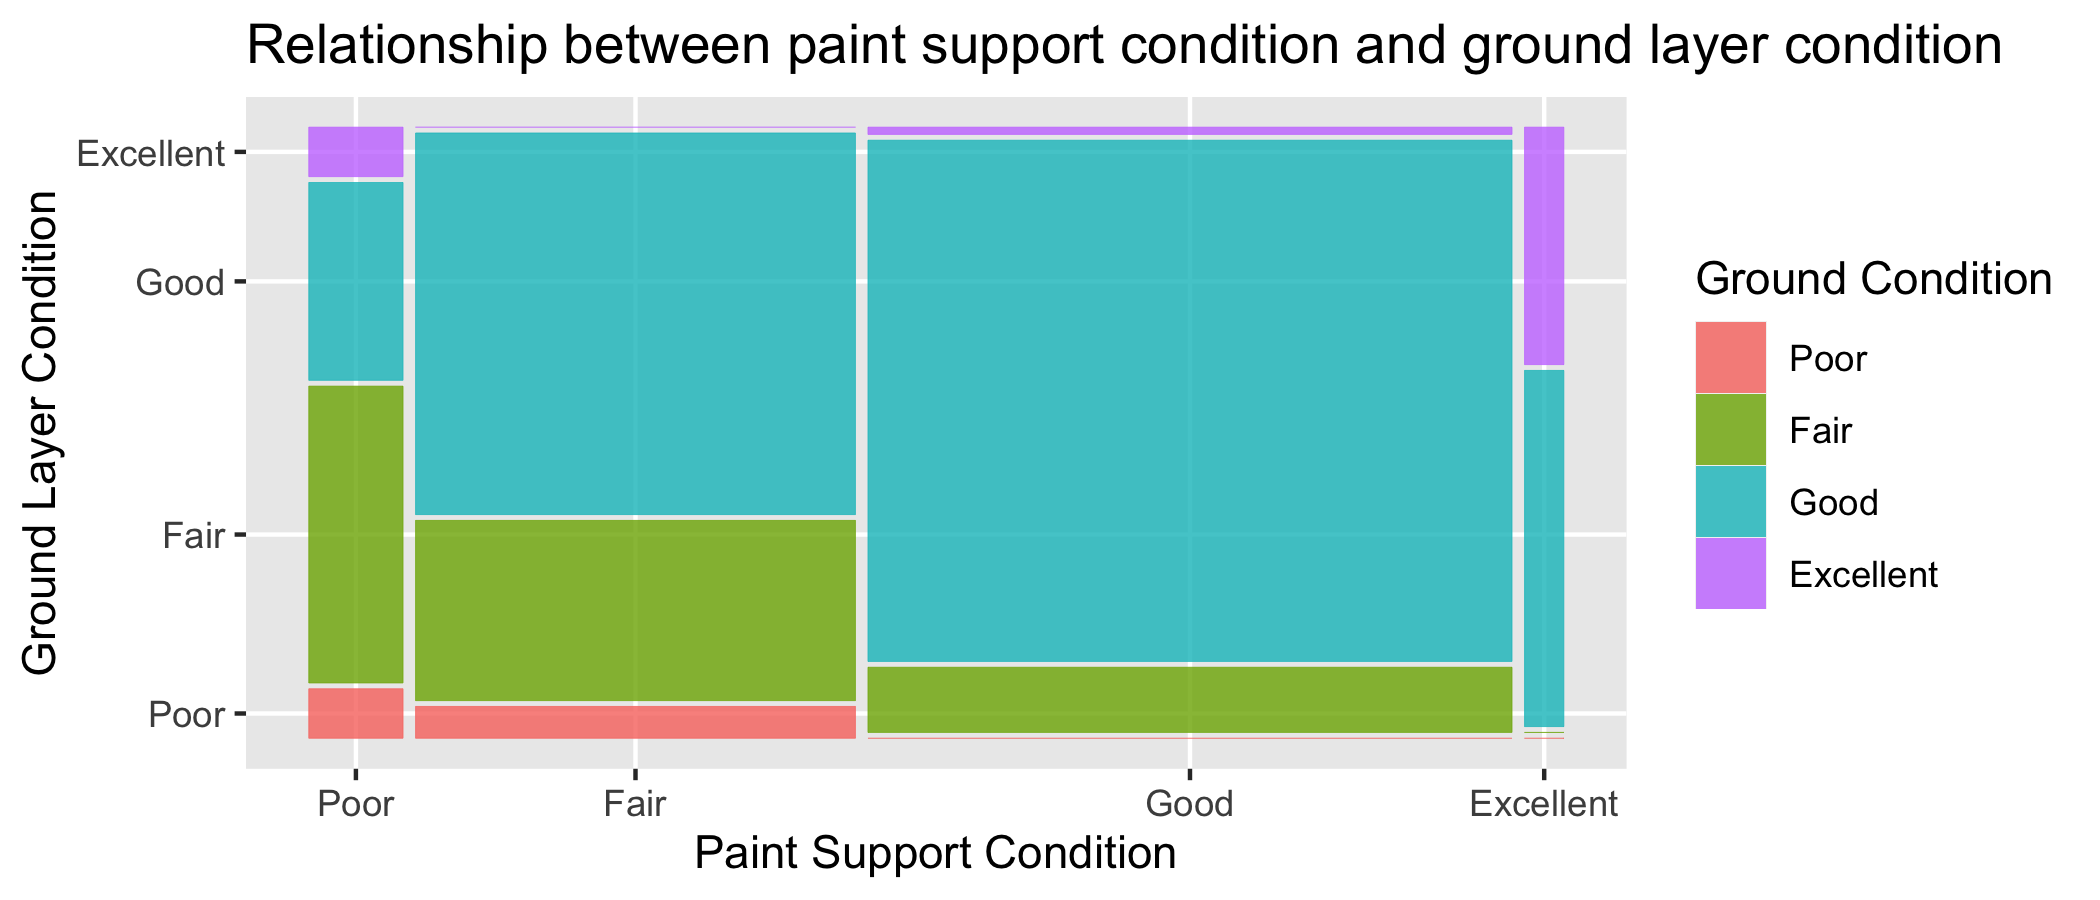
\includegraphics[scale=0.19]{images/ps_ground_mosaic.png}
    \caption{Relationship Between Paint Support Condition and Ground Condition}
    \label{ps_gr_mosaic}
\end{figure}

\begin{figure}[H]
    \centering
    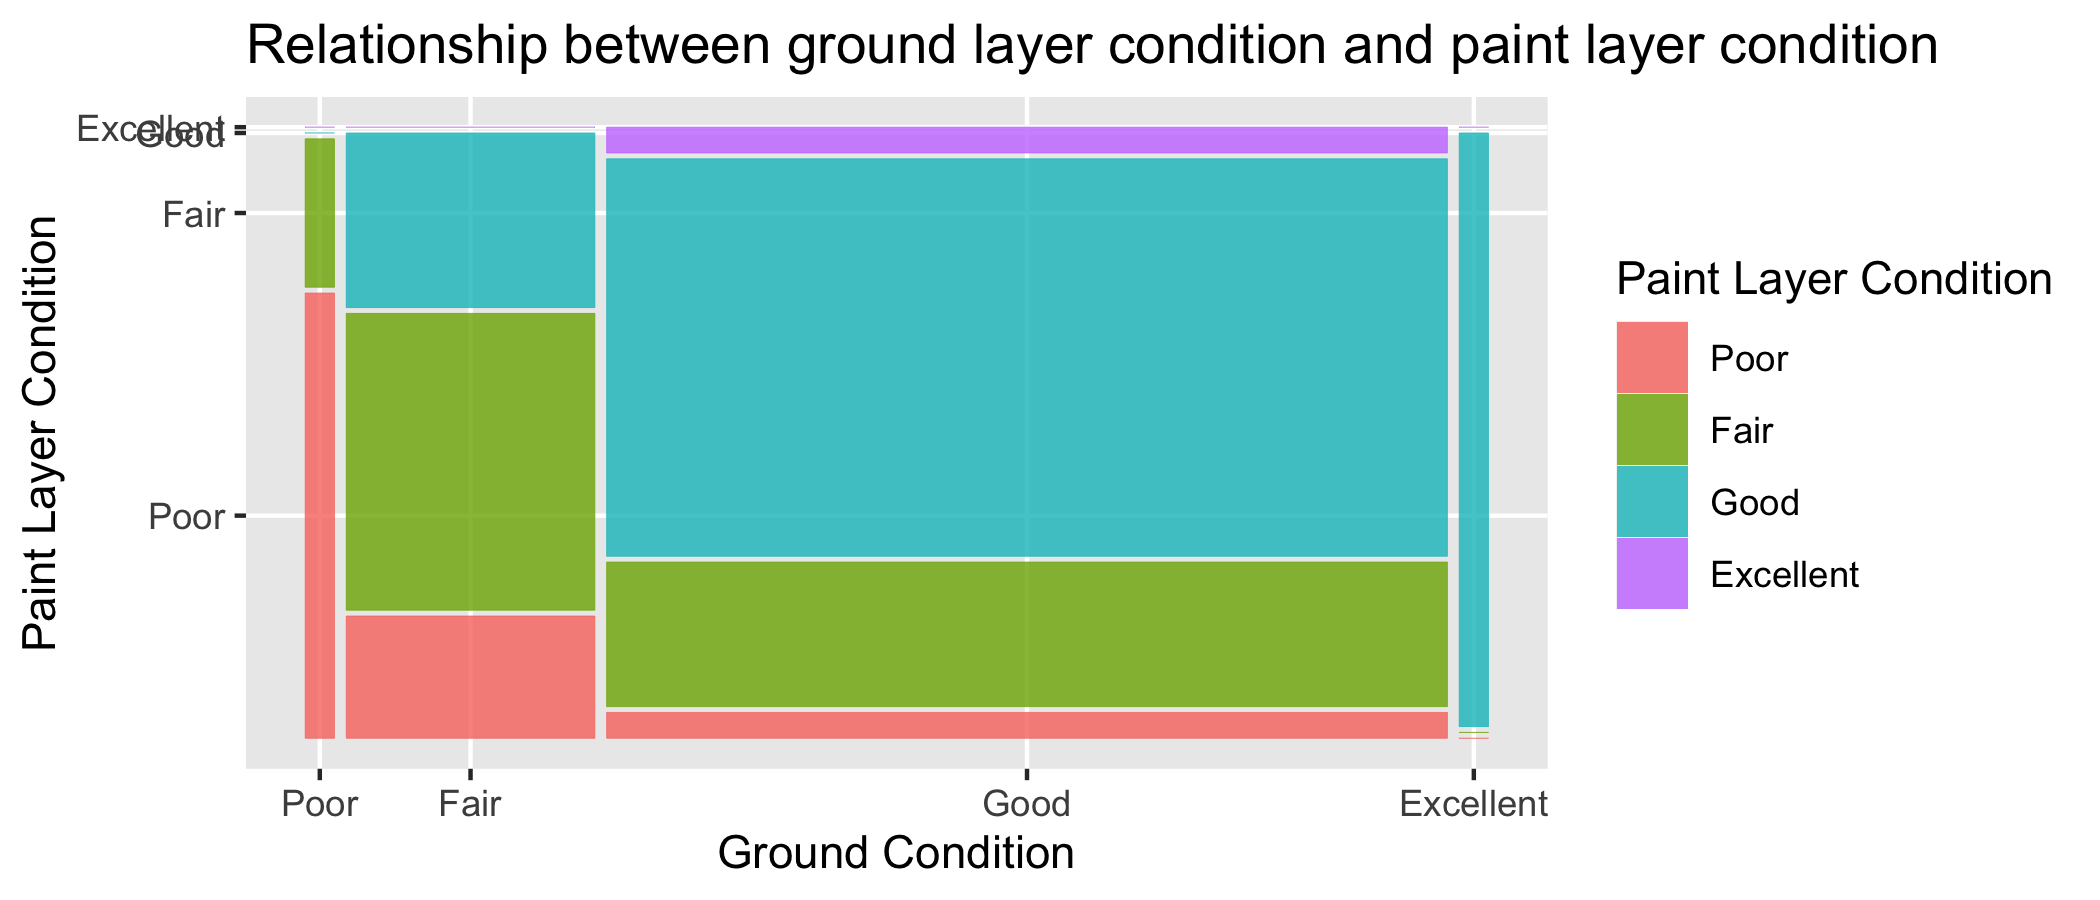
\includegraphics[scale=0.18]{images/gr_pl_mosaic.png}
    \caption{Relationship Between Ground Condition and Paint Layer Condition}
    \label{gr_pl_mosaic}
\end{figure}

\subsubsection{Relationship Between the Paint Support Condition Attributes}
This section will discuss the independence testing result between the paint support condition attributes. The testing results are presented using a tile plot as shown in Figure \ref{ps_tile}, which tries to mimic the correlation heatmap. For those whose p-value returned by the Fisher's exact test is greater than the significance level of 0.05 were labeled as blue tiles, indicating that the two condition attributes were independent. In contrast, the green tiles indicate the two attributes were related.
\begin{figure}[H]
    \centering
    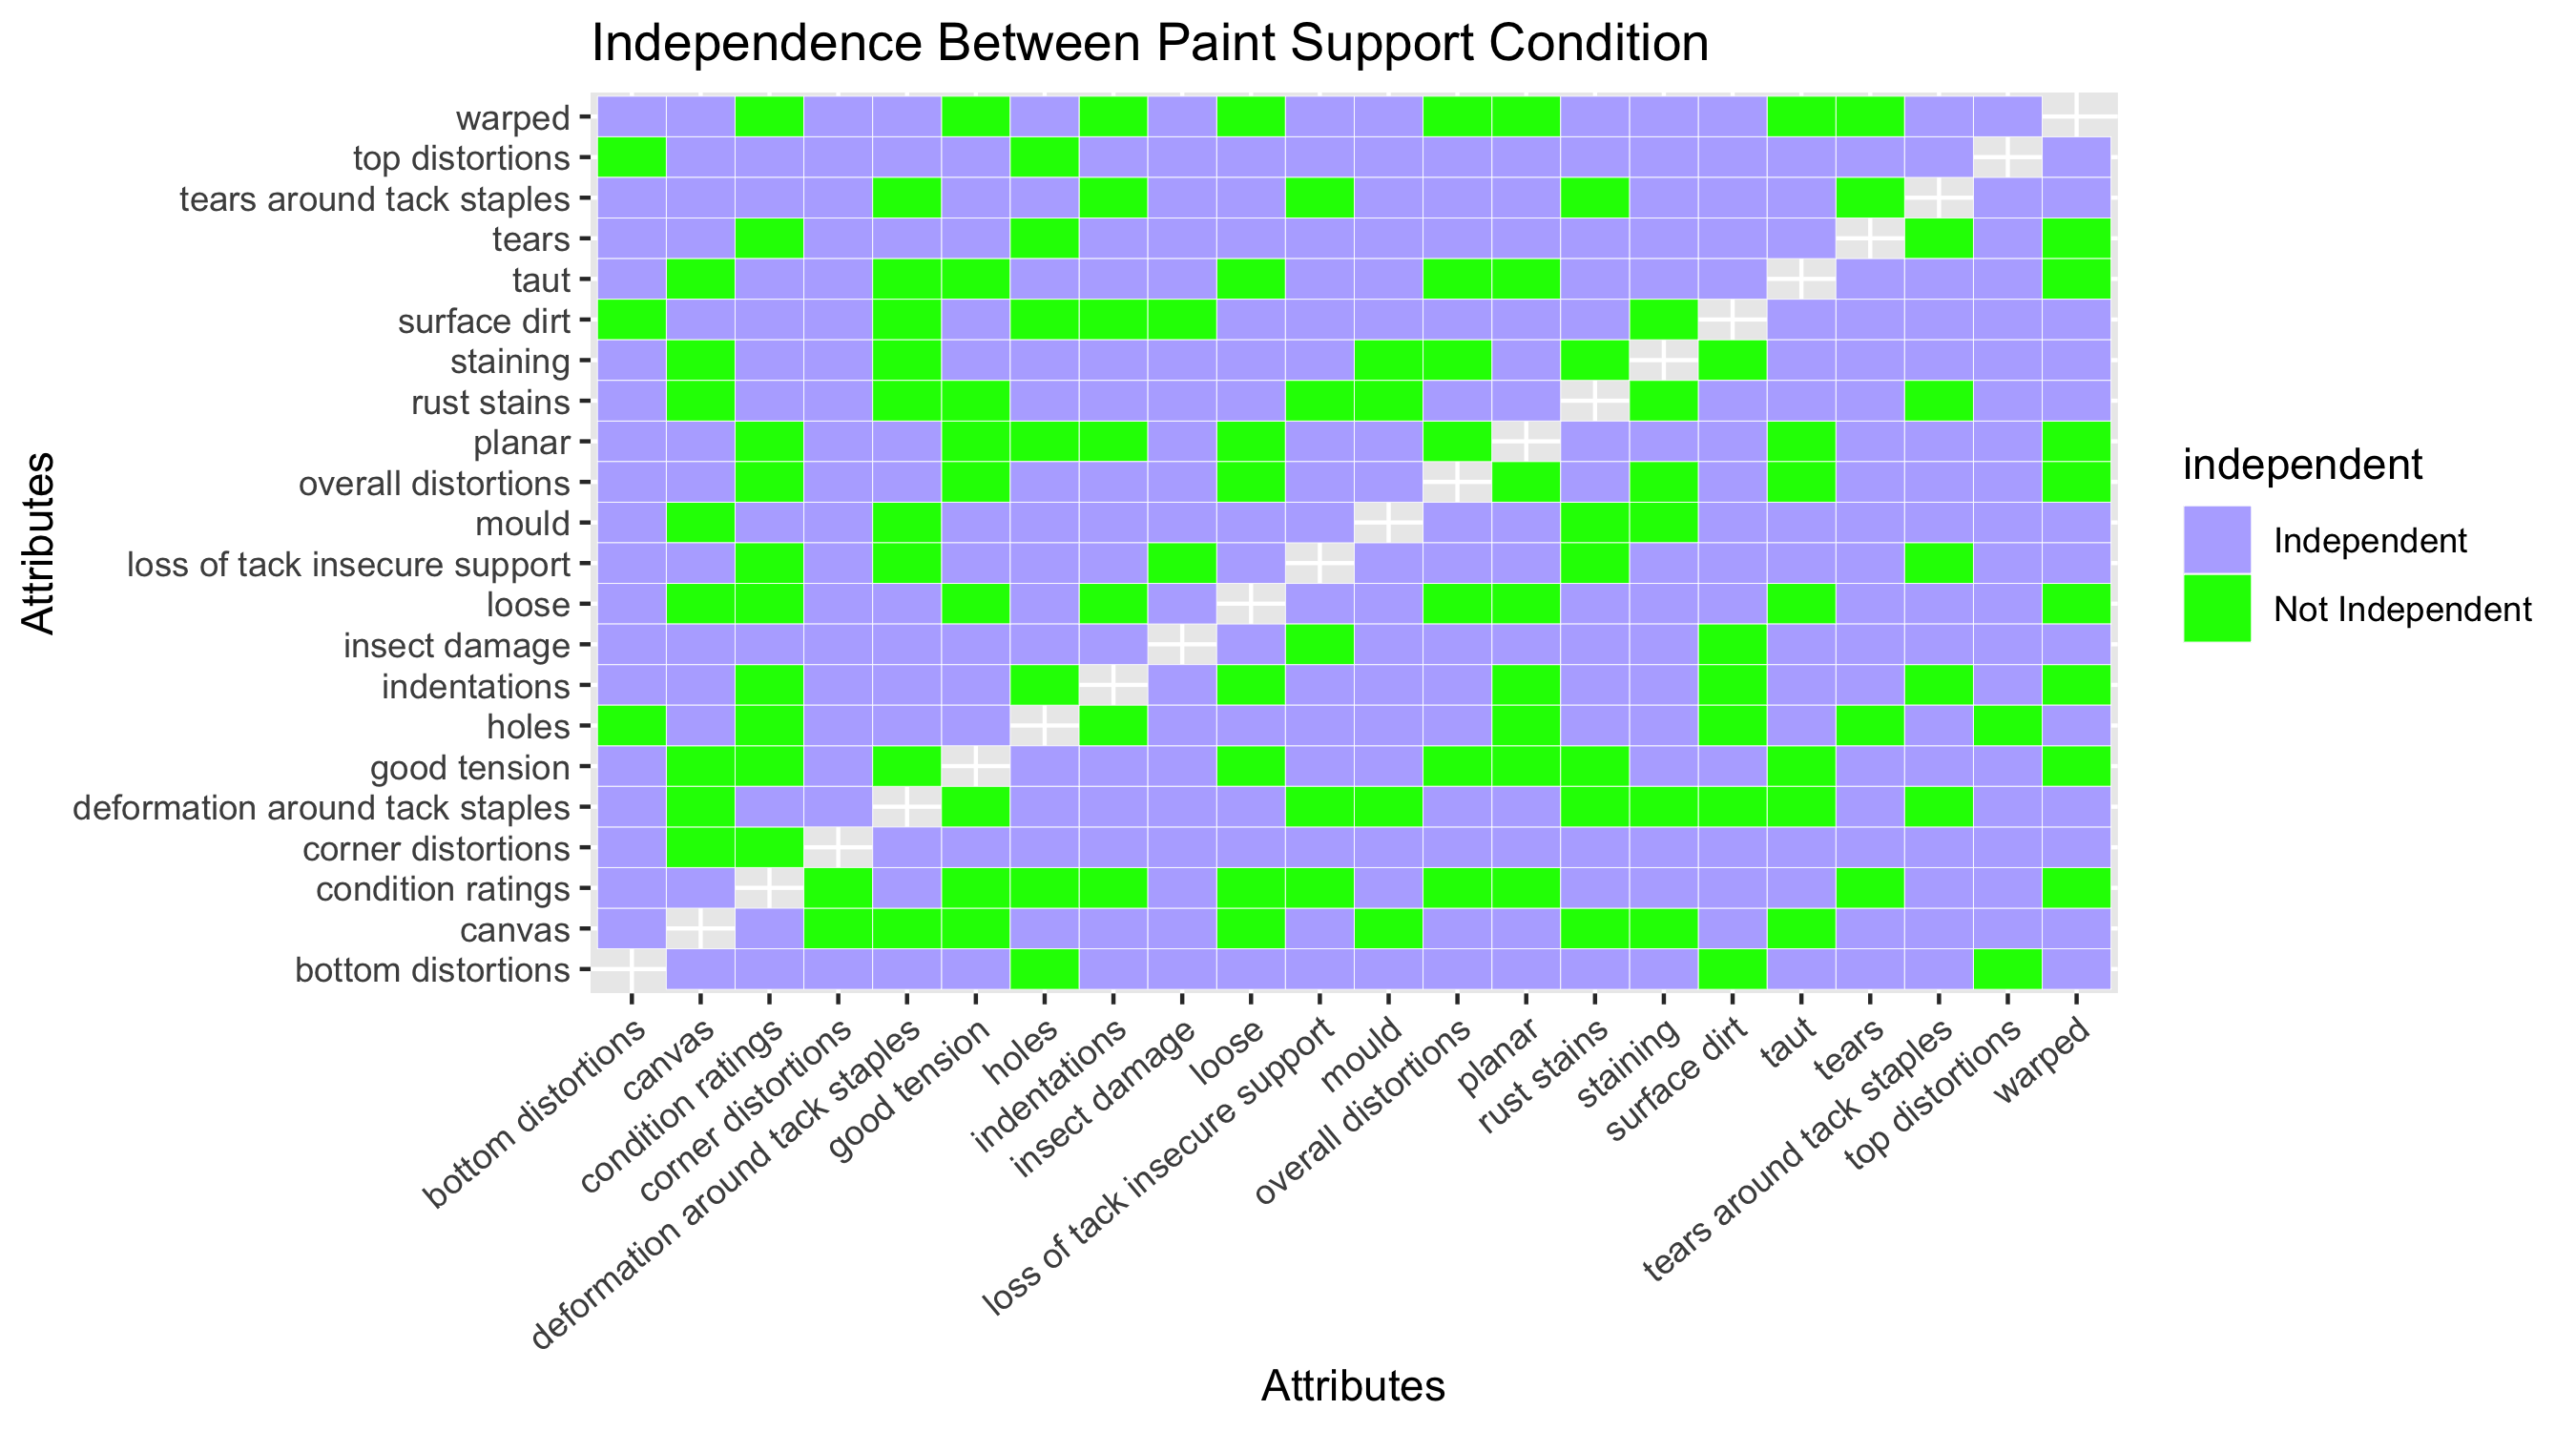
\includegraphics[scale=0.17]{images/ps_tile.png}
    \caption{Independence Between Paint Support Conditions}
    \label{ps_tile}
\end{figure}

\noindent As tile plot shown in Figure \ref{ps_tile}, we can see that the condition ratings of paint support are associated with corner distortion, good tension, holes, indentations, loose, loss of tack insecure support, overall distortions, planar, tears, and warped. Additionally, we tested relationship between the used canvas material and resulted condition of paint support to check if there is an effect to condition ratings due to the use of different materials. However, there's no statistical evidence that the two are associated. Next, we further analysed the relationship between condition ratings and the associated attributes by plotting them against each other using the mosaic plot.

\begin{figure}[H]
    \centering
    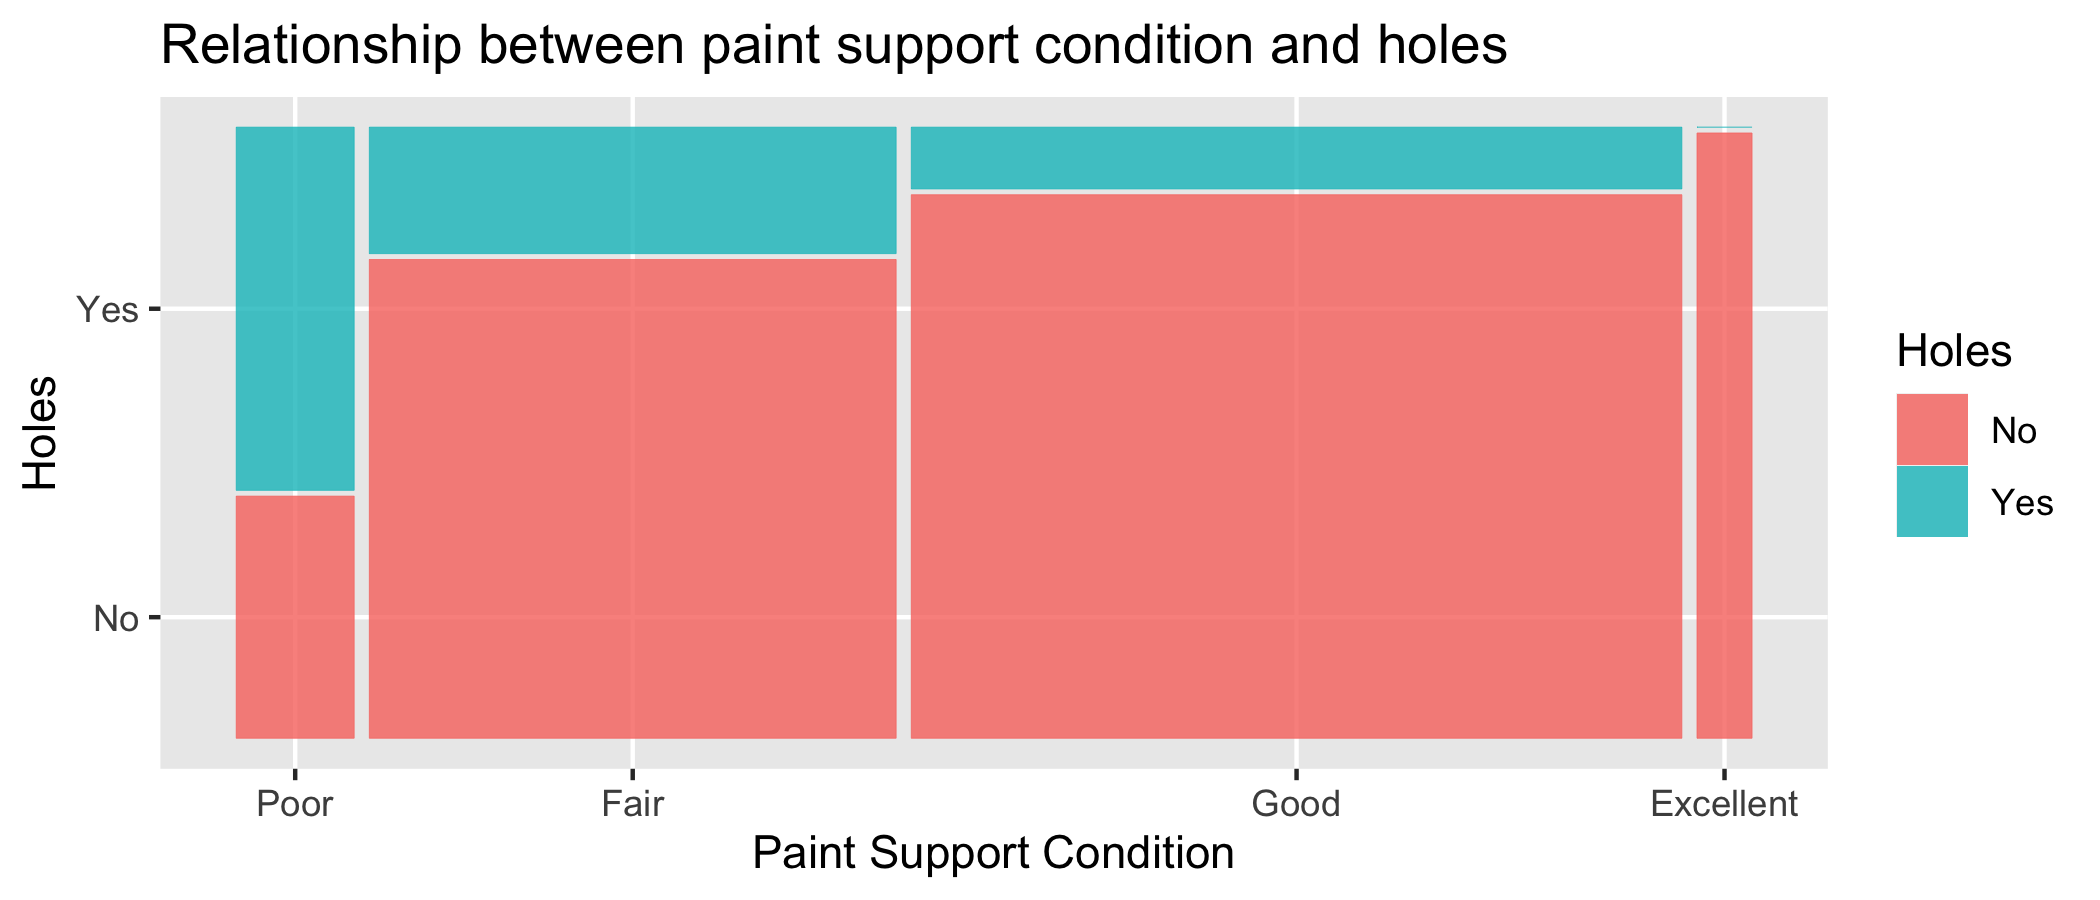
\includegraphics[scale=0.18]{images/ps_hole_mosaic.png}
    \caption{Relationship Between Paint Support Condition Ratings and Holes}
    \label{ps_hole}
\end{figure}

\noindent As Figure \ref{ps_hole} illustrates, there is a clear distinction between different support condition ratings, the proportion of paintings with no holes grows as the condition ratings increases from poor to excellent. And it is worth noting that most of the paintings were classified with fair and good condition, while poor and excellent only account for a small proportion. On top of that, similar relationship with support condition ratings could also be identified with tears, loose, corner distortion, overall distortion, indentation, and warped.

\begin{figure}[H]
    \centering
    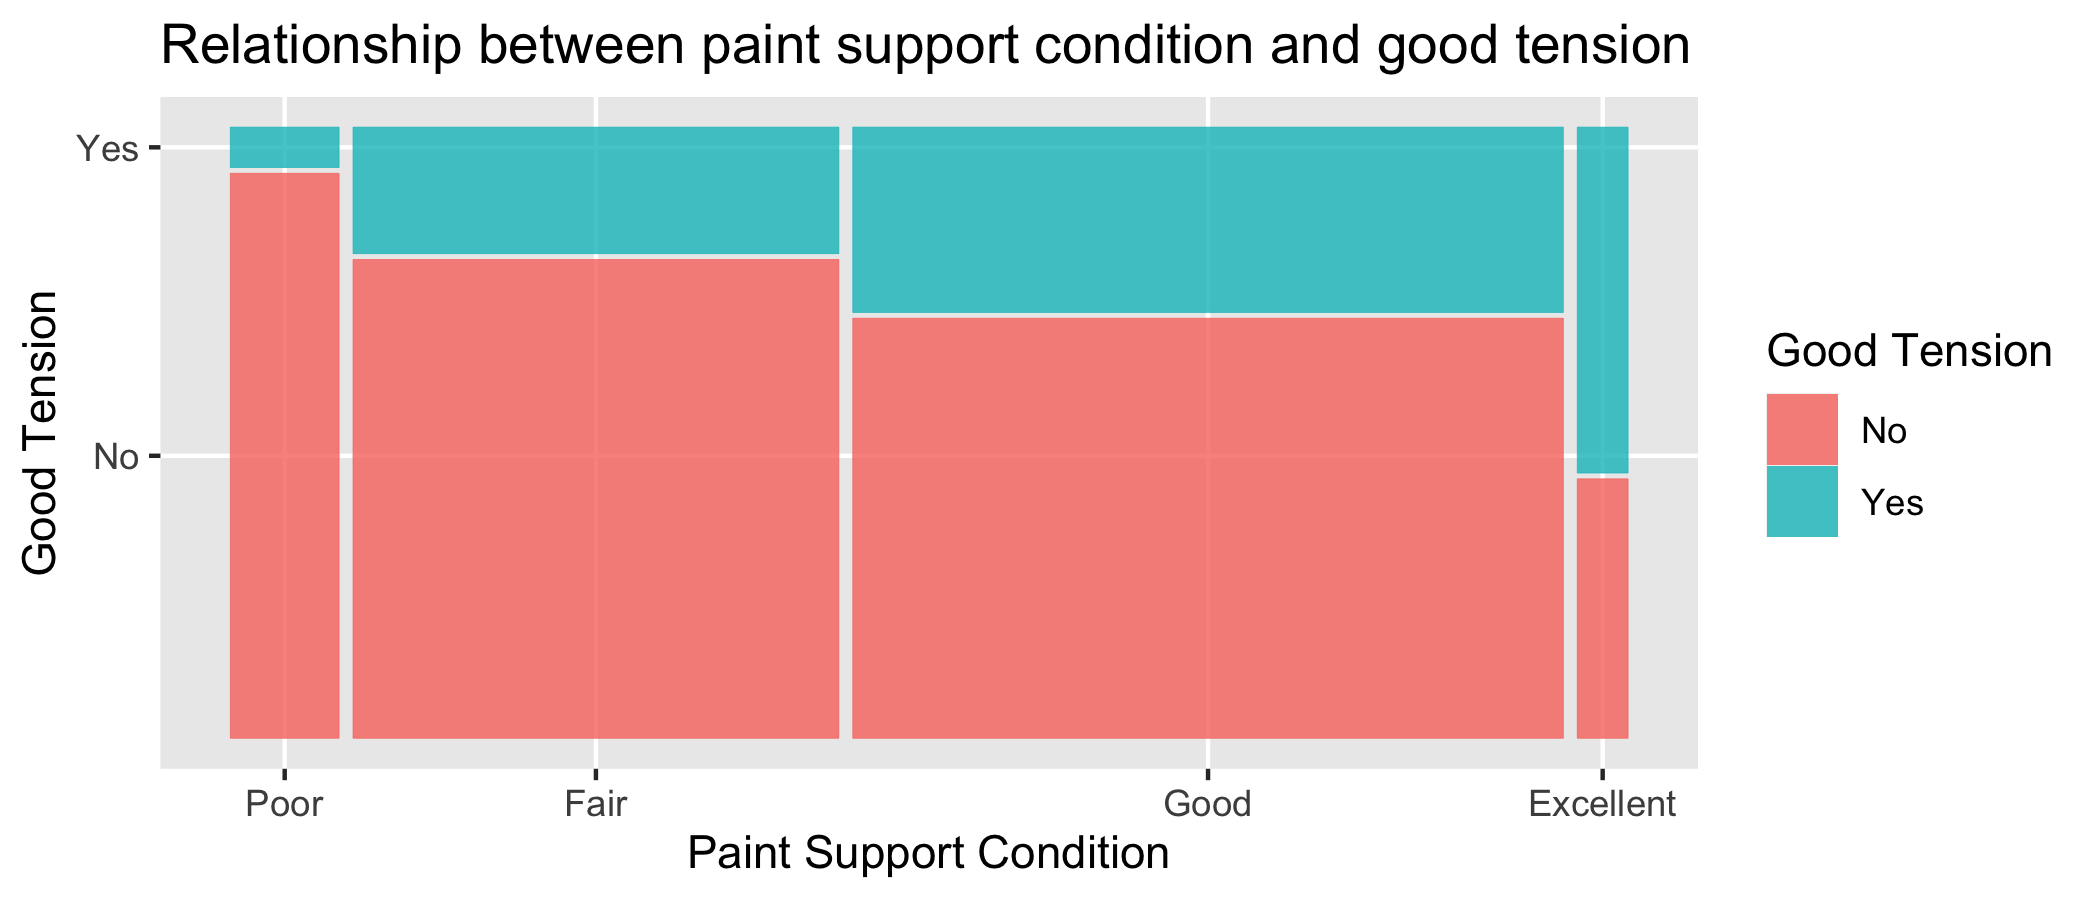
\includegraphics[scale=0.18]{images/ps_tension_mosaic.png}
    \caption{Relationship Between Paint Support Condition Ratings and Good Tension}
    \label{ps_tension}
\end{figure}

\noindent As for the relationship between paint support condition and good tension shown in Figure \ref{ps_tension}, we can see a clear differentiation with the previous plot, it is no surprise that, as the support condition ratings increases from poor to excellent, the proportion of paintings with good tension also increases. Although the Fisher's exact test did not show that the support condition ratings were associated with taut, but similar trend could also be seen with the two.
\bigbreak
\noindent Here we further investigate the relationship between insect damage and surface dirt in paint support shown in Figure \ref{insect_dirt}. It is worth noting that when a painting has no insect damage, there is an even chance to have surface dirt present. On the other hand, when there is insect damage present in a painting, likely, surface dirt will also appear. However, we need to mention that paintings with insect damage only account for a small proportion of the sample population. To make the conclusion, we may need more samples to reduce the non-response bias.

\begin{figure}[H]
    \centering
    \captionsetup{justification=centering}
    \begin{minipage}{0.5\textwidth}
        \centering
        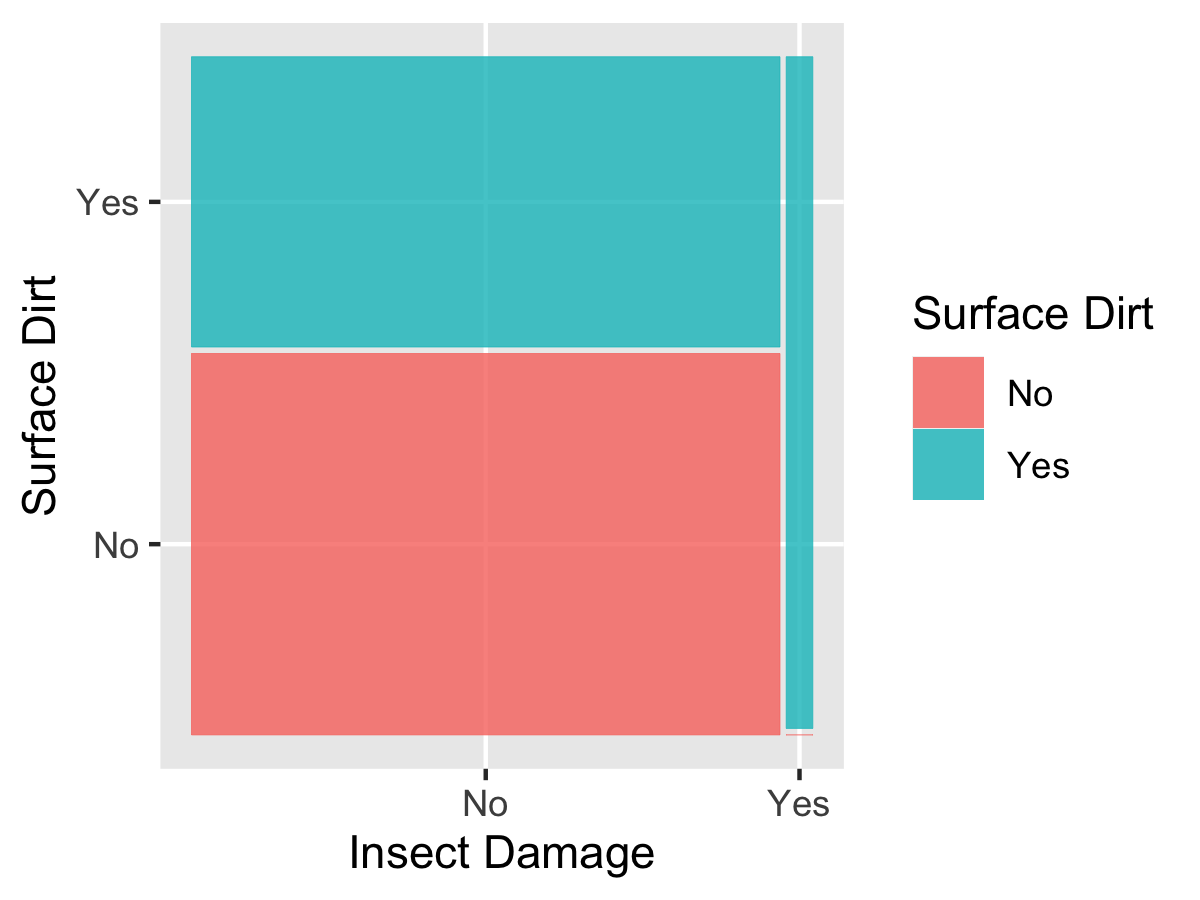
\includegraphics[width=1\textwidth]{images/insect_dirt_mosaic.png} 
        \caption{Relationship Between Insect Damage and Surface Dirt}
        \label{insect_dirt}
    \end{minipage}\hfill
    \begin{minipage}{0.5\textwidth}
        \centering
        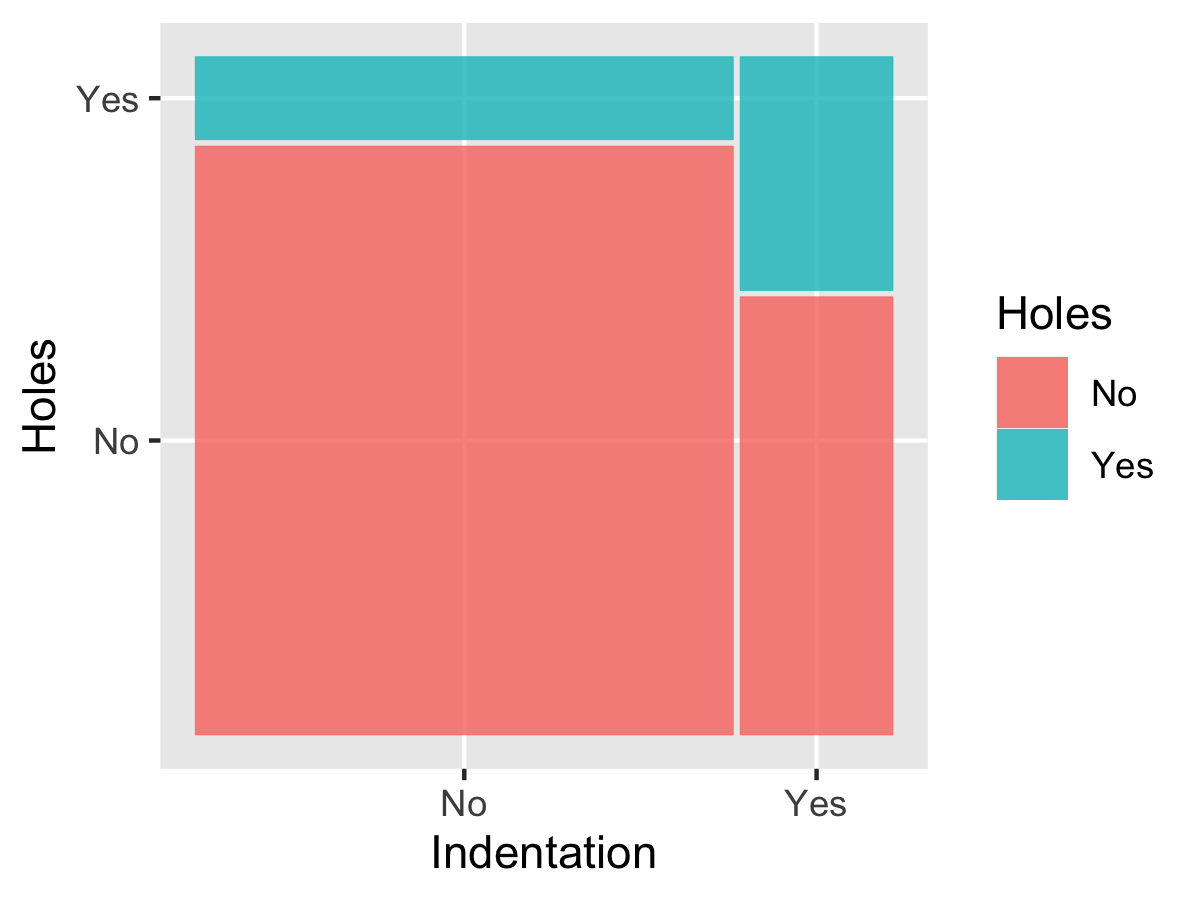
\includegraphics[width=1\textwidth]{images/indent_holes_mosaic.png} 
        \caption{Relationship Between Indentation and Holes}
        \label{indent_holes}
    \end{minipage}
\end{figure}

\noindent As for the association between indentation and holes shown in Figure \ref{indent-holes}, a painting with indentation will also have a higher chance to have holes than those paintings without indentation. In fact, after estimating odds, under the study condition, paintings with indentation having holes are almost 3.78 times higher than for paintings with no indentation.

\subsubsection{Relationship Between the Ground Layer Condition Attributes}
This section will discuss the associations between the ground layer condition attributes. Again, the outcome of the Fisher's exact test will be presented using the tile plot.

\begin{figure}[H]
    \centering
    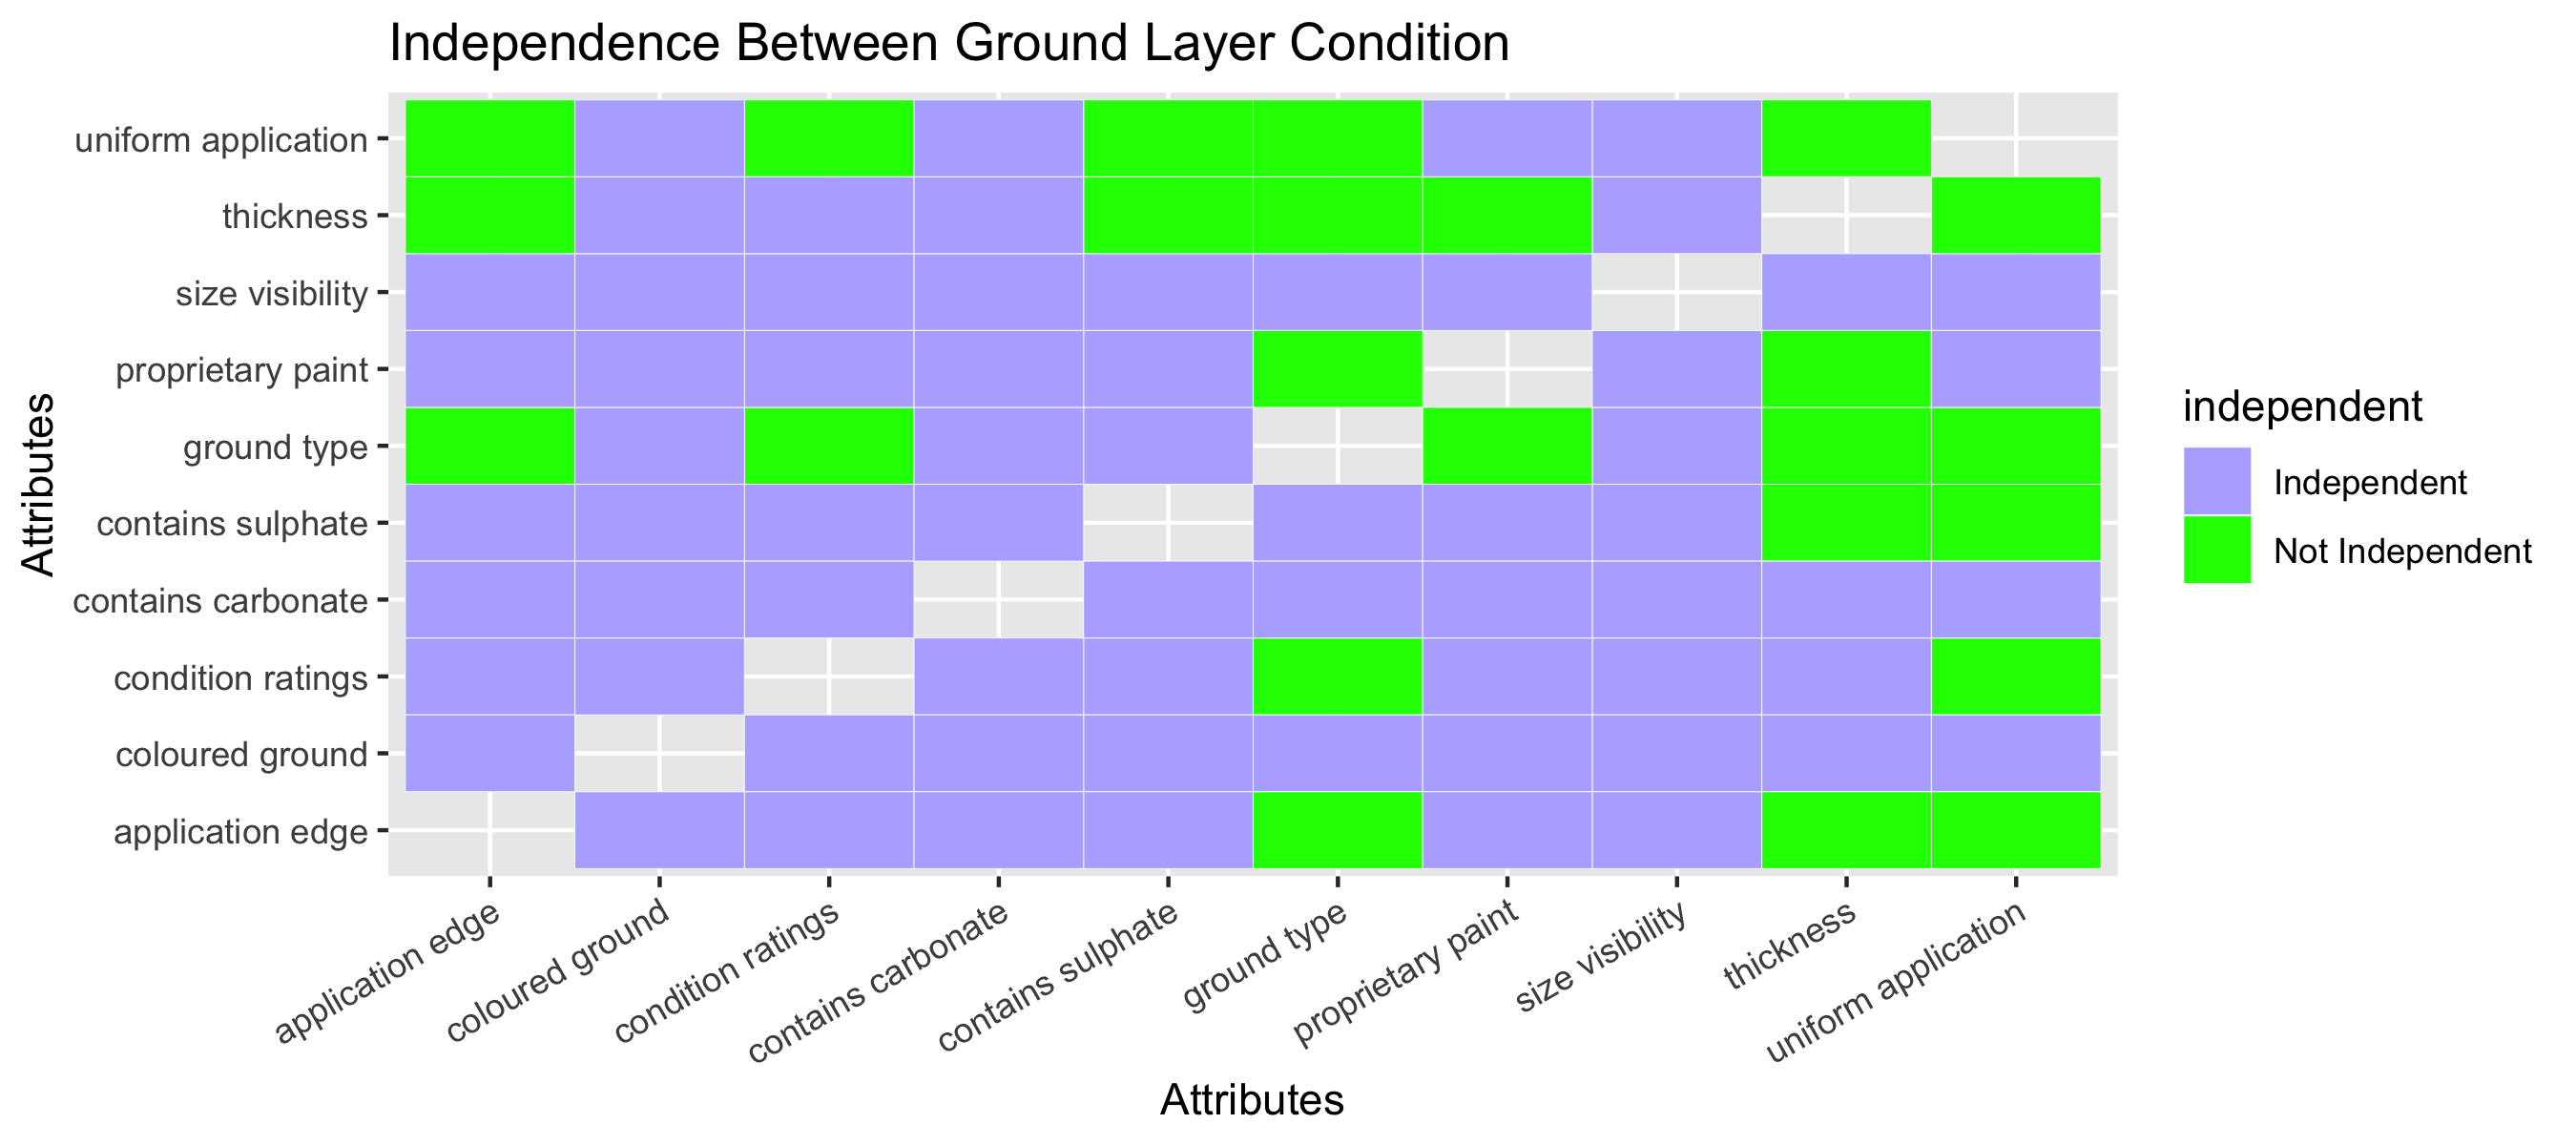
\includegraphics[scale=0.15]{images/gr_tile.png}
    \caption{Independence Between Ground Layer Conditions}
    \label{gr_tile}
\end{figure}

\noindent As Figure \ref{gr_tile} depicts, there are only two attributes that are associated with the ground condition ratings, namely, ground type and uniform application. Figure \ref{gr_type} shows the relationship between different ground type and the ground condition ratings. As mentioned in the introduction, due to material shortage in early 20th century, local artists without access to commercial materials starts to source their own material instead. Here we can see that commercial ground tend to have higher proportion paintings being classified as good and excellent. After computing the odds ratio, we found that the odds of a painting having a good or excellent condition in the commercial ground group is about two times higher than in the artist applied ground group.

\begin{figure}[H]
    \centering
    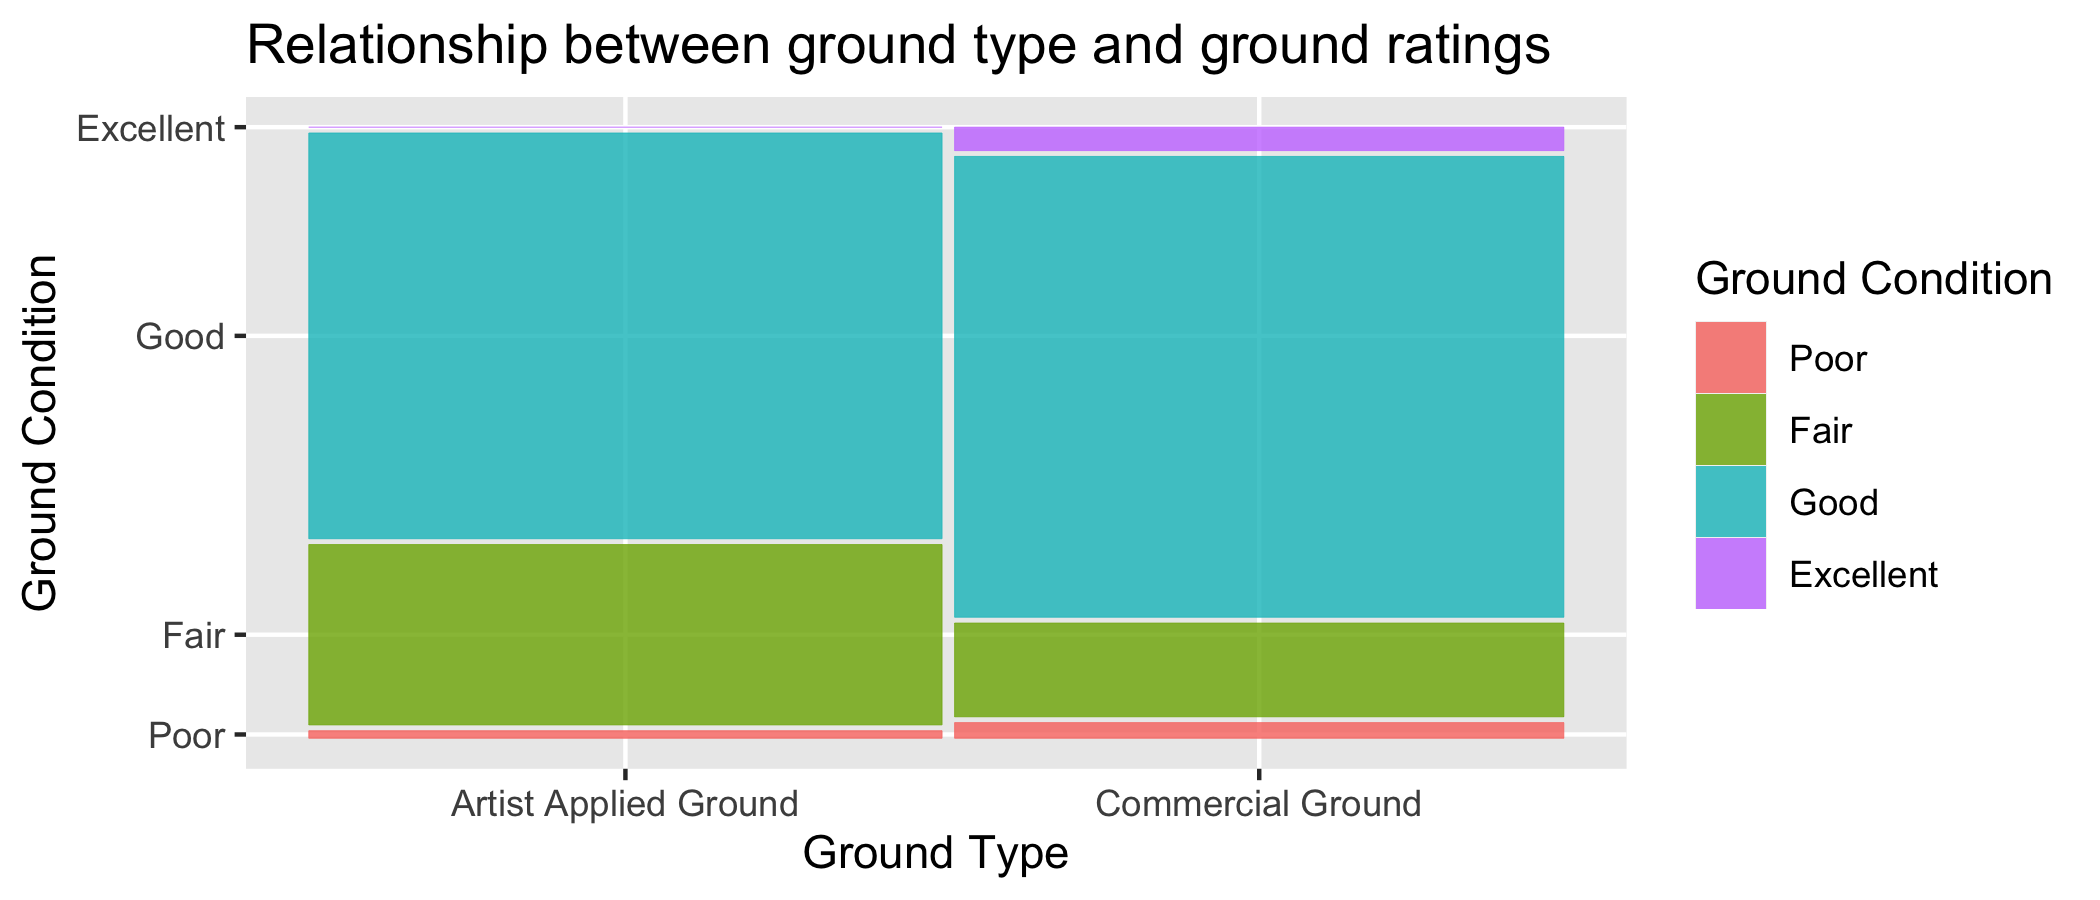
\includegraphics[scale=0.17]{images/gr_type.png}
    \caption{Relationship Between Ground Condition and Different Ground Type}
    \label{gr_type}
\end{figure}

\noindent Moreover, we can notice that the ground types are associated with the thickness of the applied ground. As we can see from Figure \ref{gr_thickness}, the proportion of the ground being thickly applied for artist applied ground is almost three times that on commercial ground.

\begin{figure}[H]
    \centering
    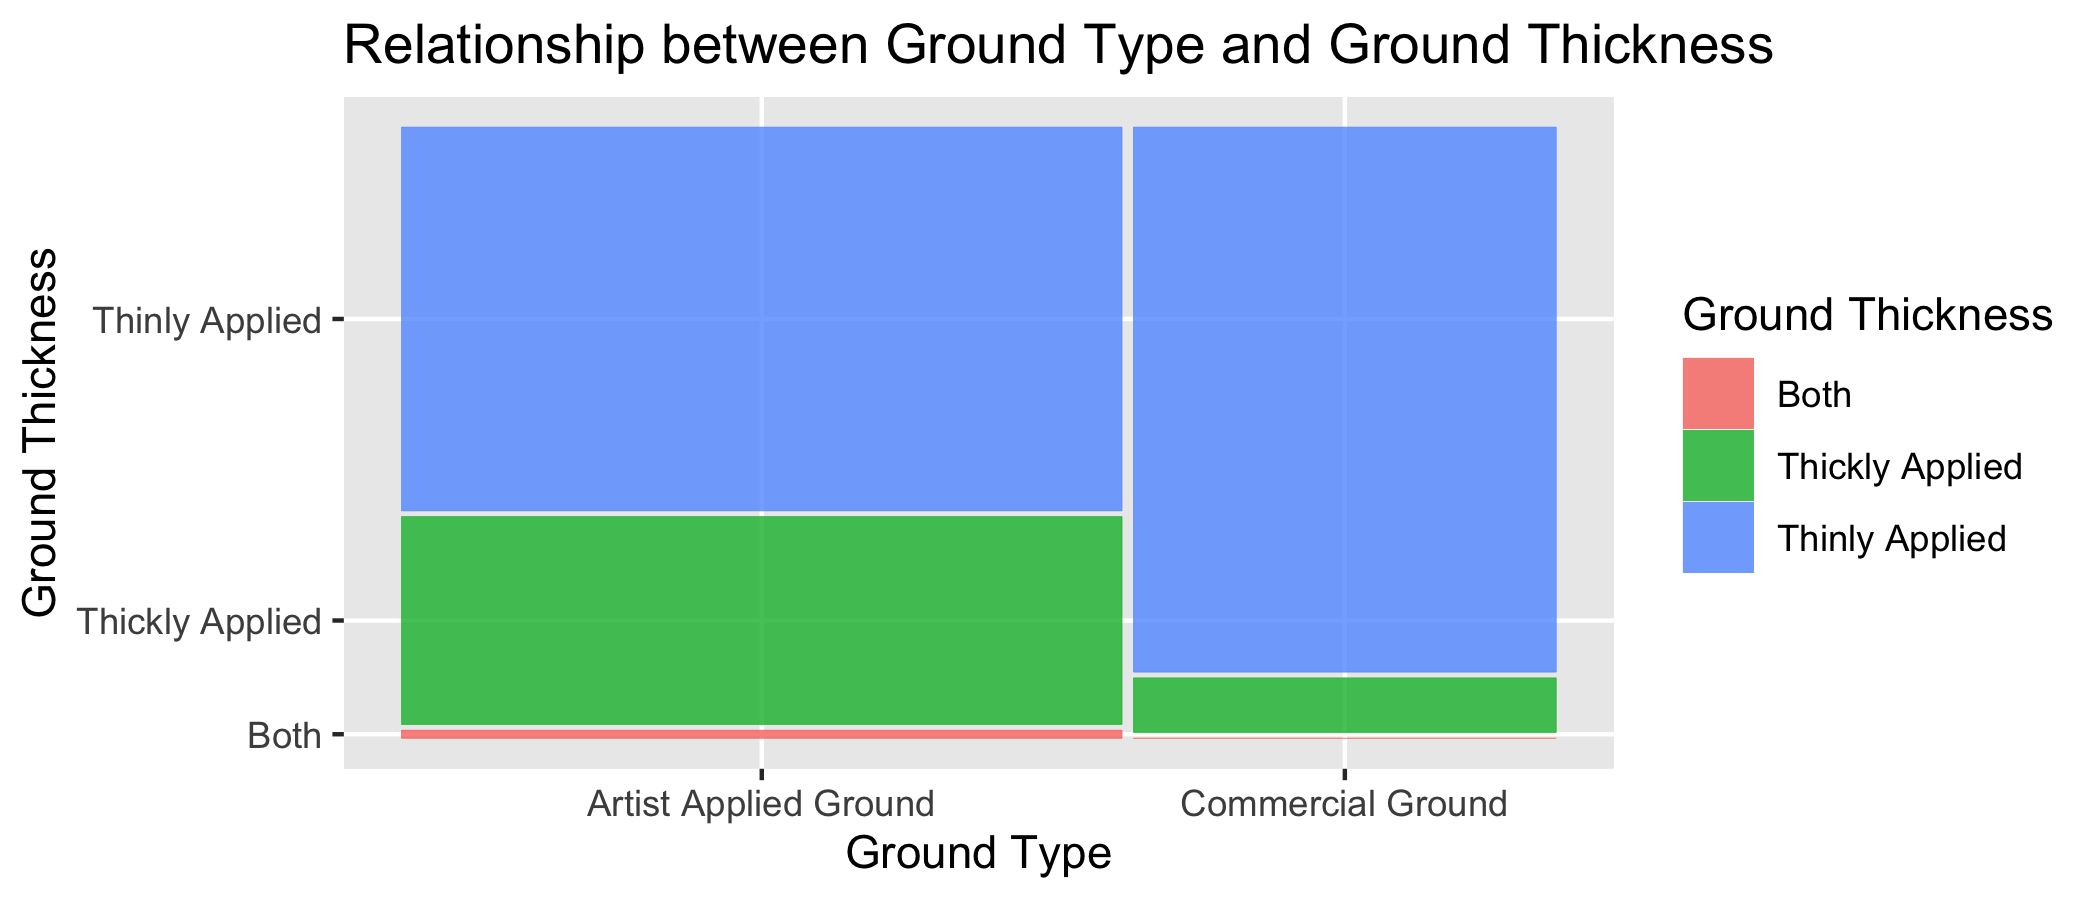
\includegraphics[scale=0.17]{images/type_thickness.png}
    \caption{Relationship Between Ground Type and Ground Layer Thickness}
    \label{gr_thickness}
\end{figure}

\noindent Since the ground type and uniform application are related to each other. We can see that there is a clear contrast between paintings with artist applied ground and paintings with commercial ground in Figure \ref{gr_uniform}, as paintings with commercial ground are about seven times more likely to have their ground to be uniformly applied on than the one with artist applied ground.

\begin{figure}[H]
    \centering
    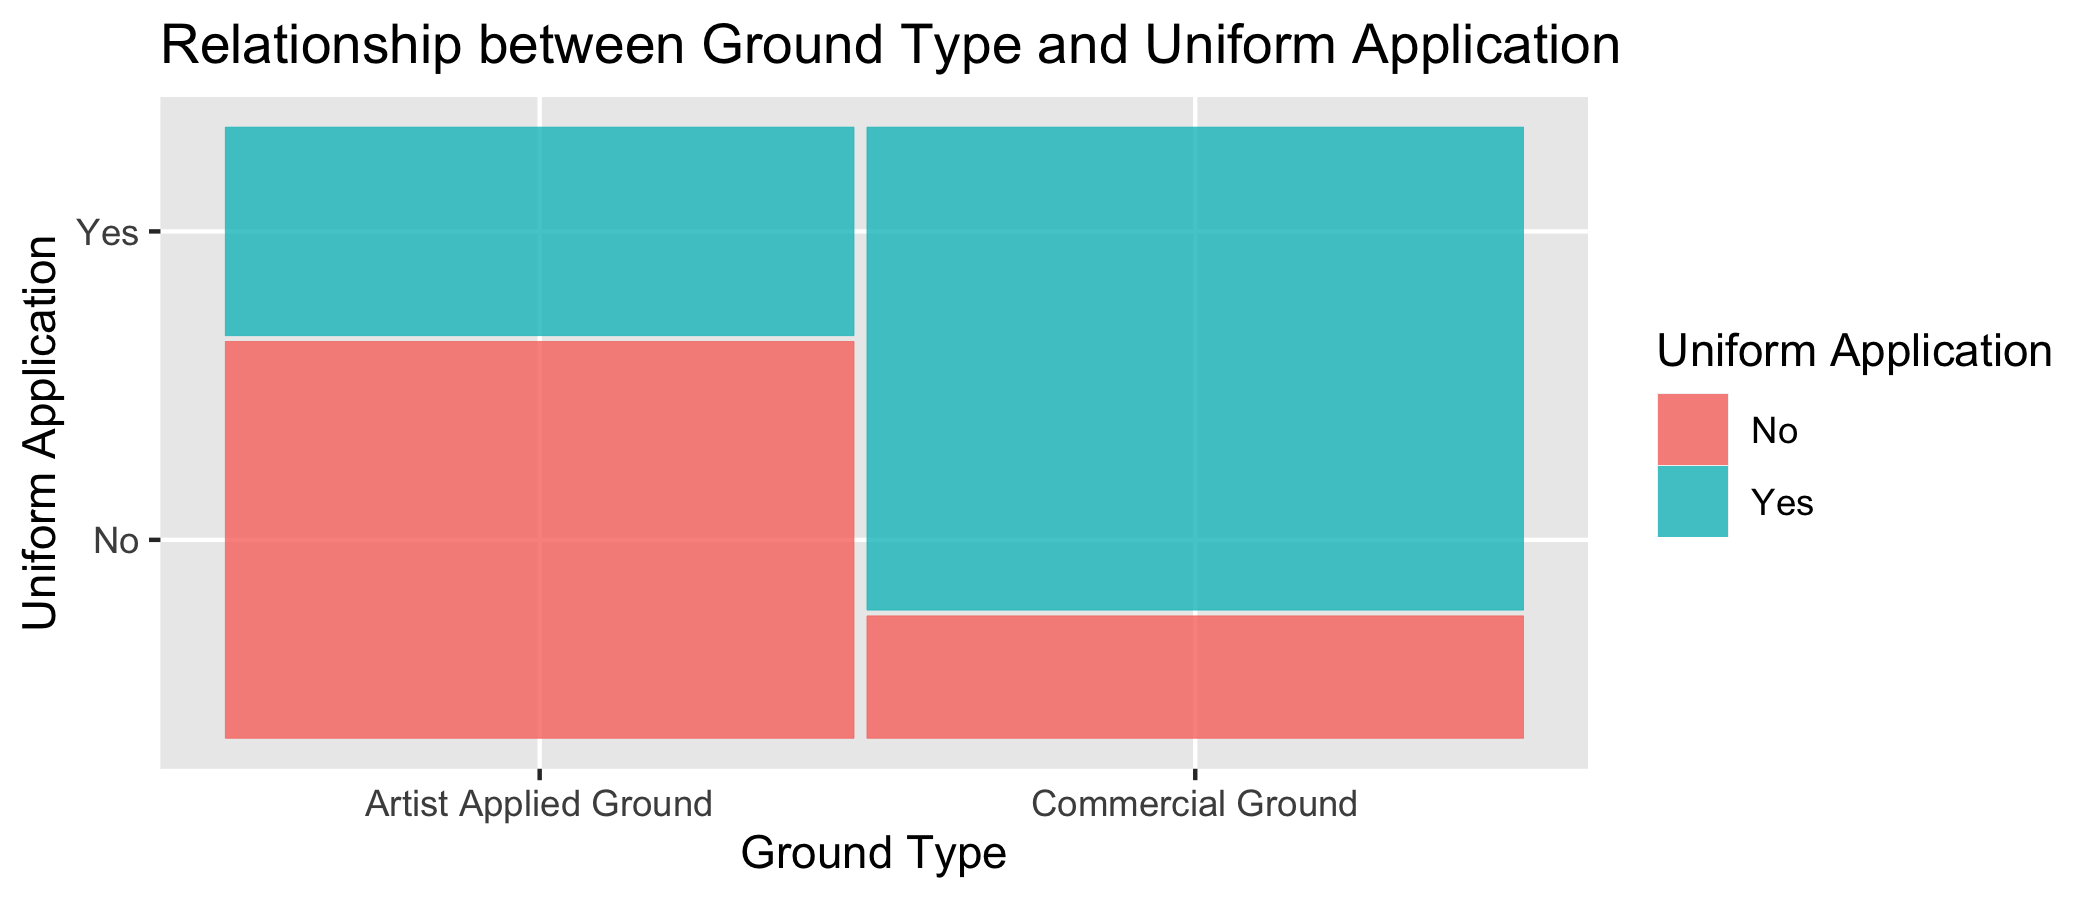
\includegraphics[scale=0.15]{images/type_uniform.png}
    \caption{Relationship Between Uniform Applied Ground and Ground Type}
    \label{gr_uniform}
\end{figure}

\subsubsection{Relationship Between the Paint Layer Attributes}
In this section, we will further testing the association between the paint layer attributes. As per previous independence testing, the testing results were presented as tile plot, where green tile indicates association, while blue tiles indicates independence. 

\begin{figure}[H]
    \centering
    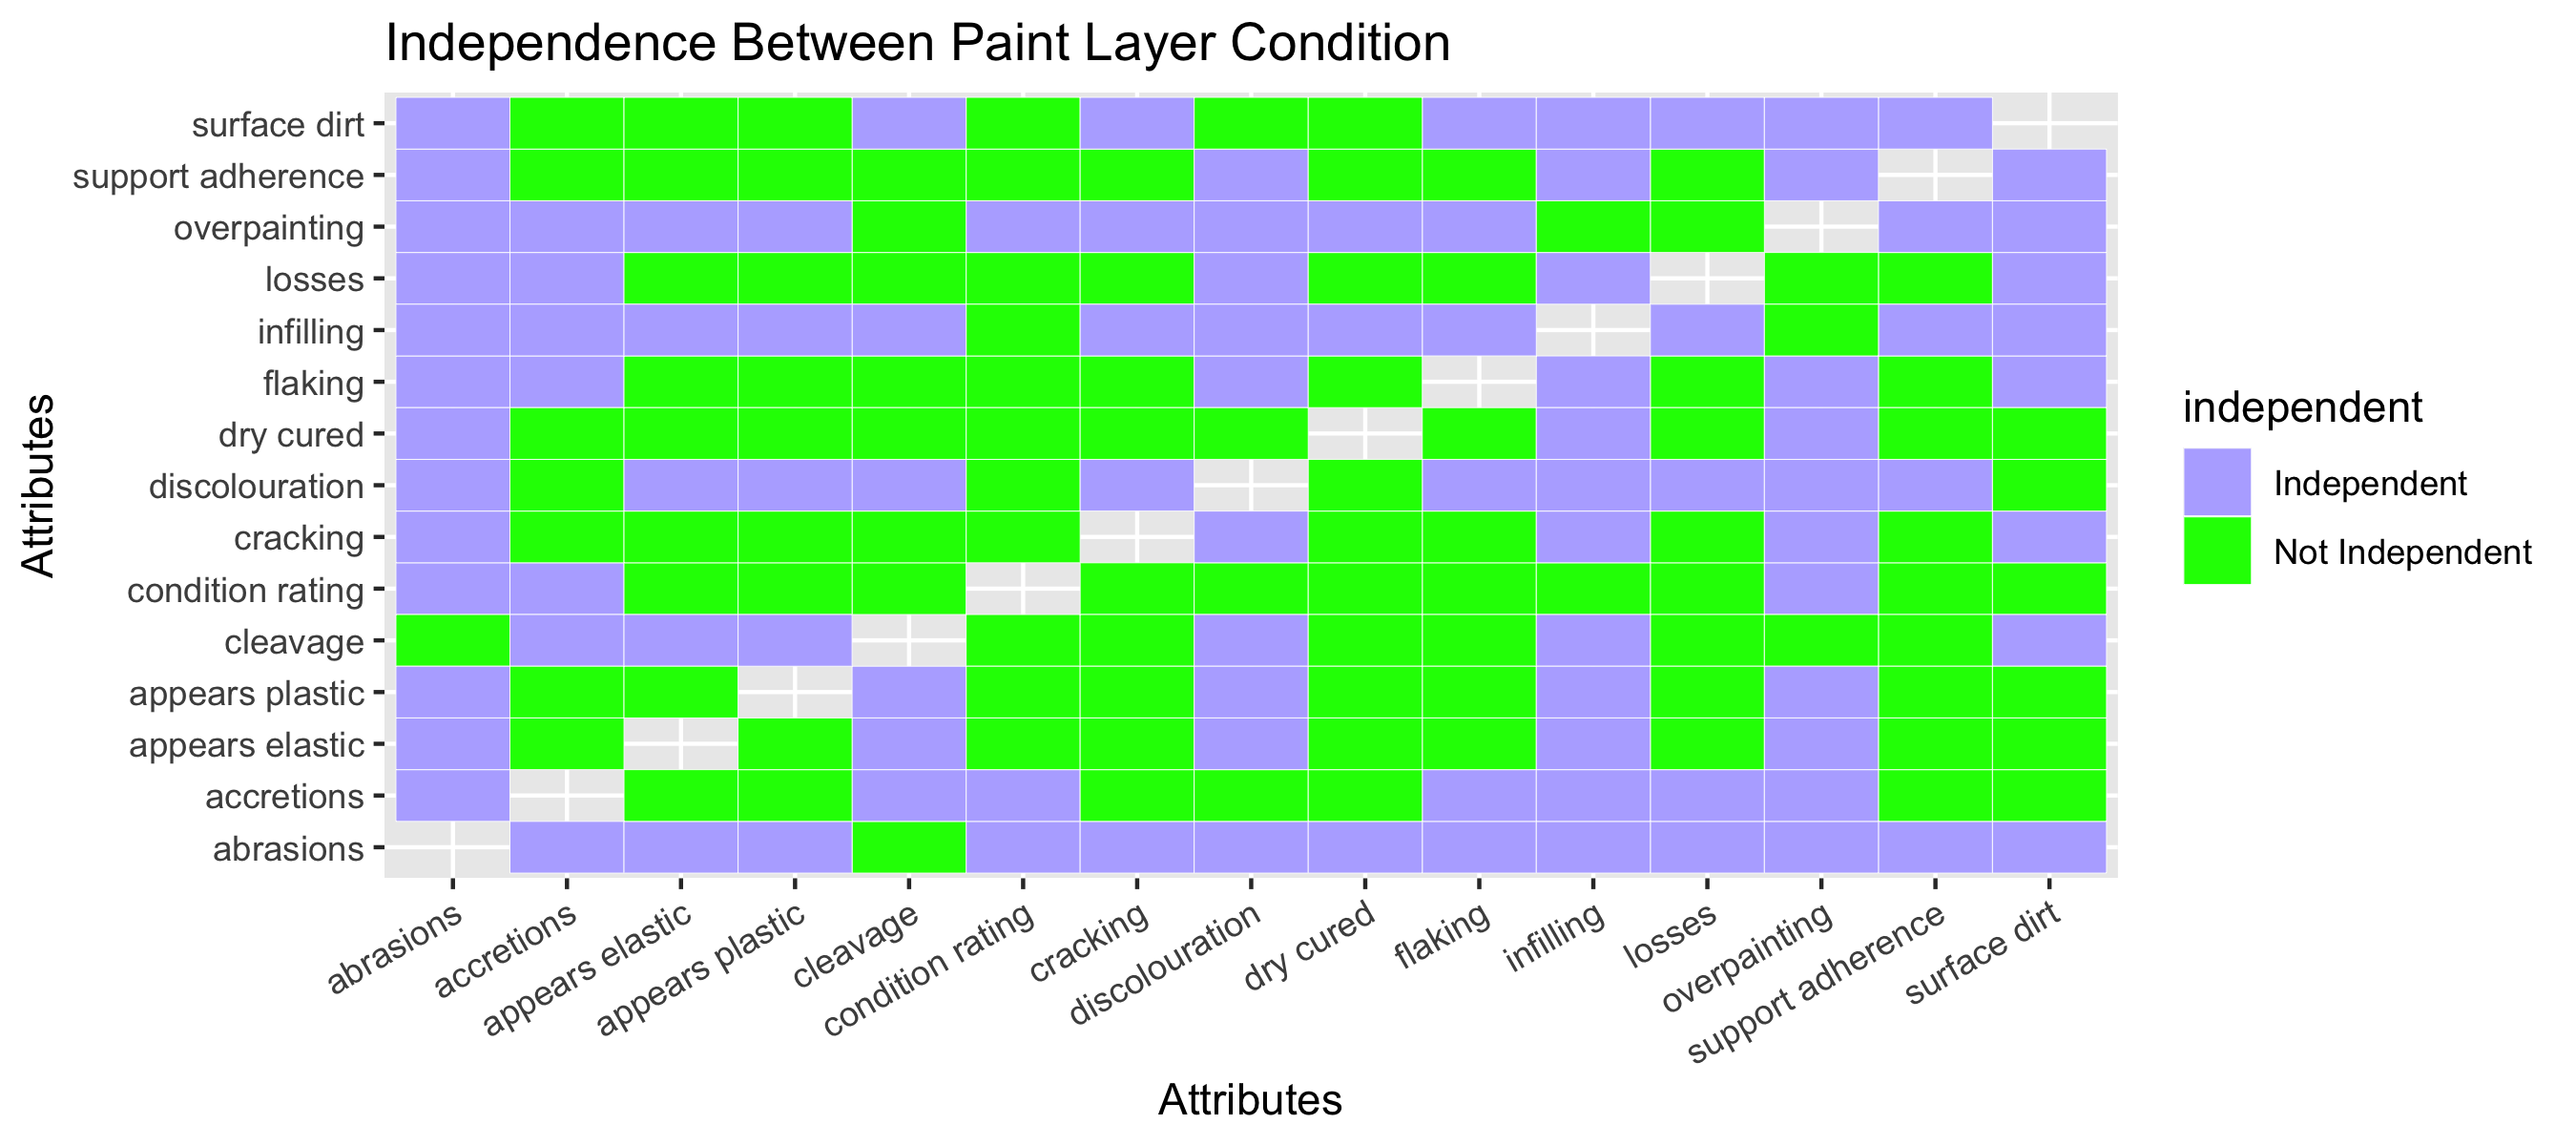
\includegraphics[scale=0.17]{images/pl_tile.png}
    \caption{Independence Between Paint Layer Conditions}
    \label{pl_tile}
\end{figure}

\noindent As we can see from Figure \ref{pl_tile}, the test results suggests that paint layer condition ratings are associated with elasticness and plasticness of the layer, cleavage, cracking, discolouration, dry cured, flaking, infilling, losses, support adherence, and surface dirt of the layer. 

\begin{figure}[H]
    \centering
    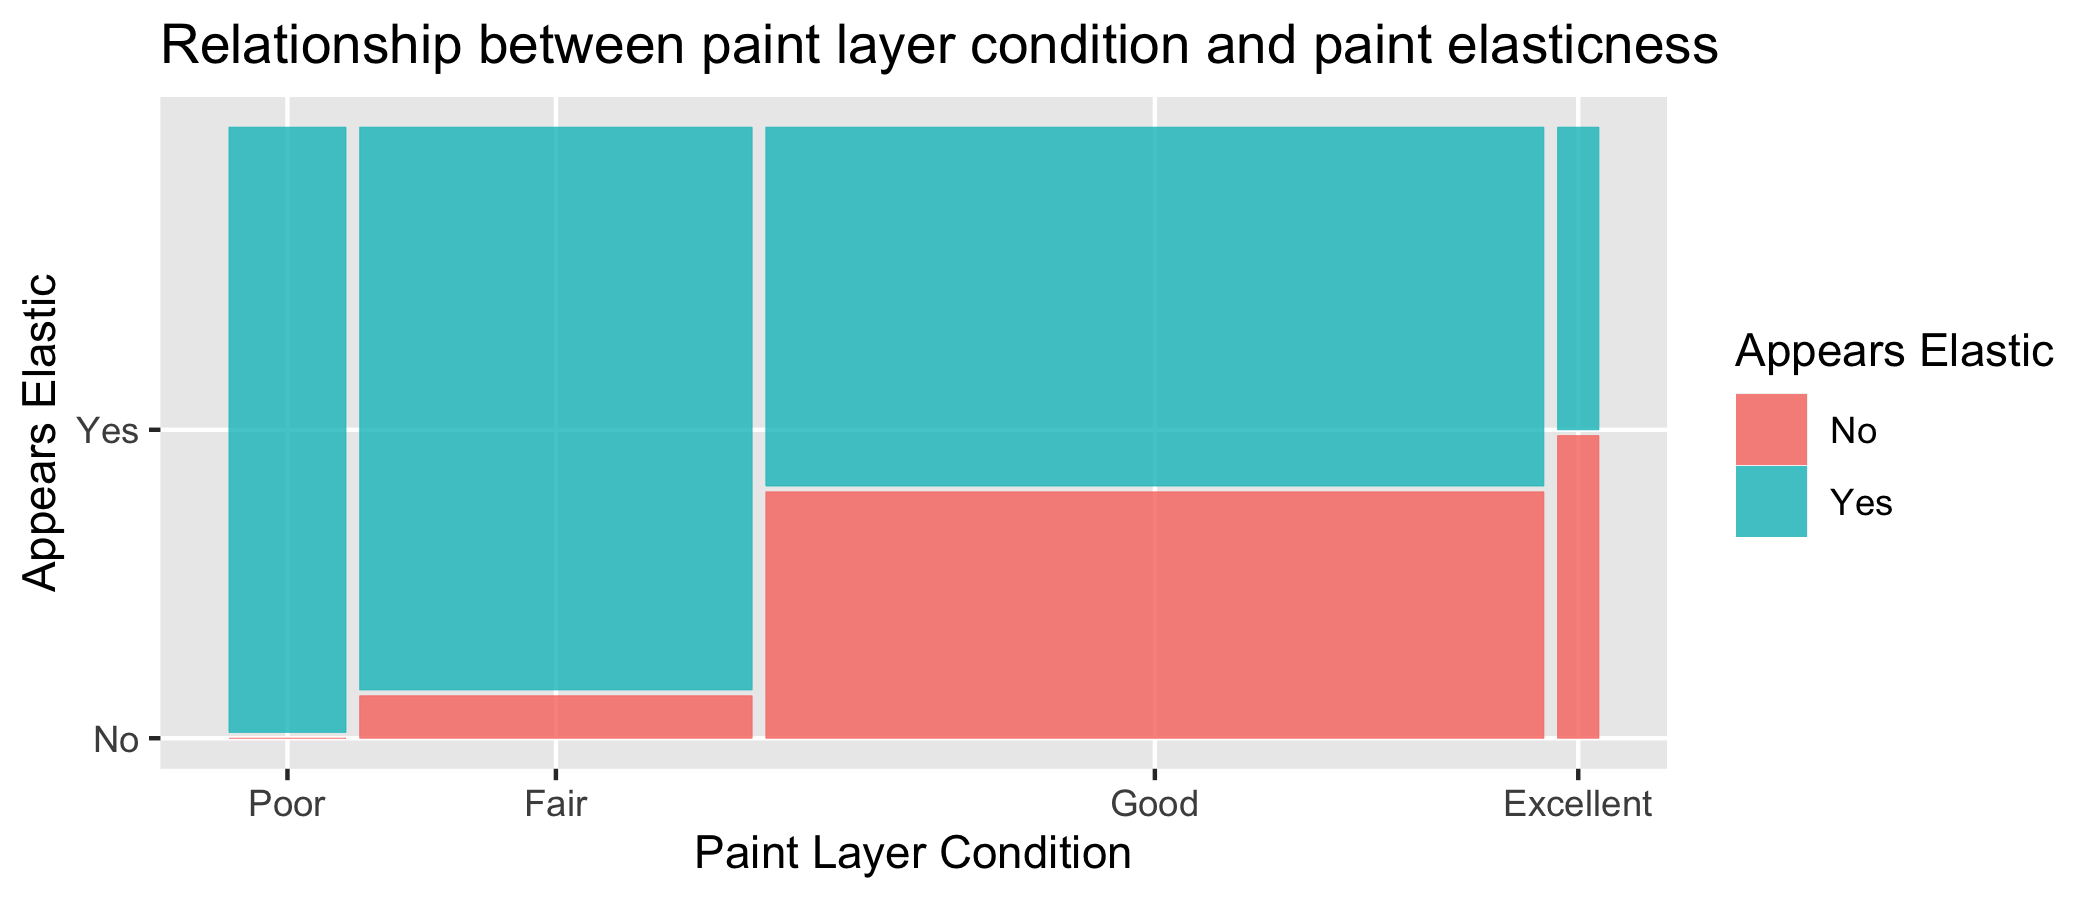
\includegraphics[scale=0.2]{images/pl_elastic.png}
    \caption{Relationship Between Paint Layer Condition and Paint Elasticness}
    \label{pl_elastic}
\end{figure}

\noindent Figure \ref{pl_elastic} visualises the relationship between paint layer condition and the elasticness of the painting. The height of the box shows the conditional proportion of paintings with elastic paint layer given the paint layer condition ratings, the plot clearly brings out paintings with poor layer condition will highly likely to appear elastic. Nevertheless, a clear trend could be seen as the proportion of paintings that appears to be elastic decreases as the paint layer condition ratings increases from poor to excellent, where the proportion of paintings does not appear elastic is considerably higher when condition ratings is excellent. 
\bigbreak
\noindent And it is worth pointing out that similar relationship with the layer condition can also be seen on cleavage, paint cracking, paint discolouration, dry cured, flaking, losses, and surface dirt of the layer.

\begin{figure}[H]
    \centering
    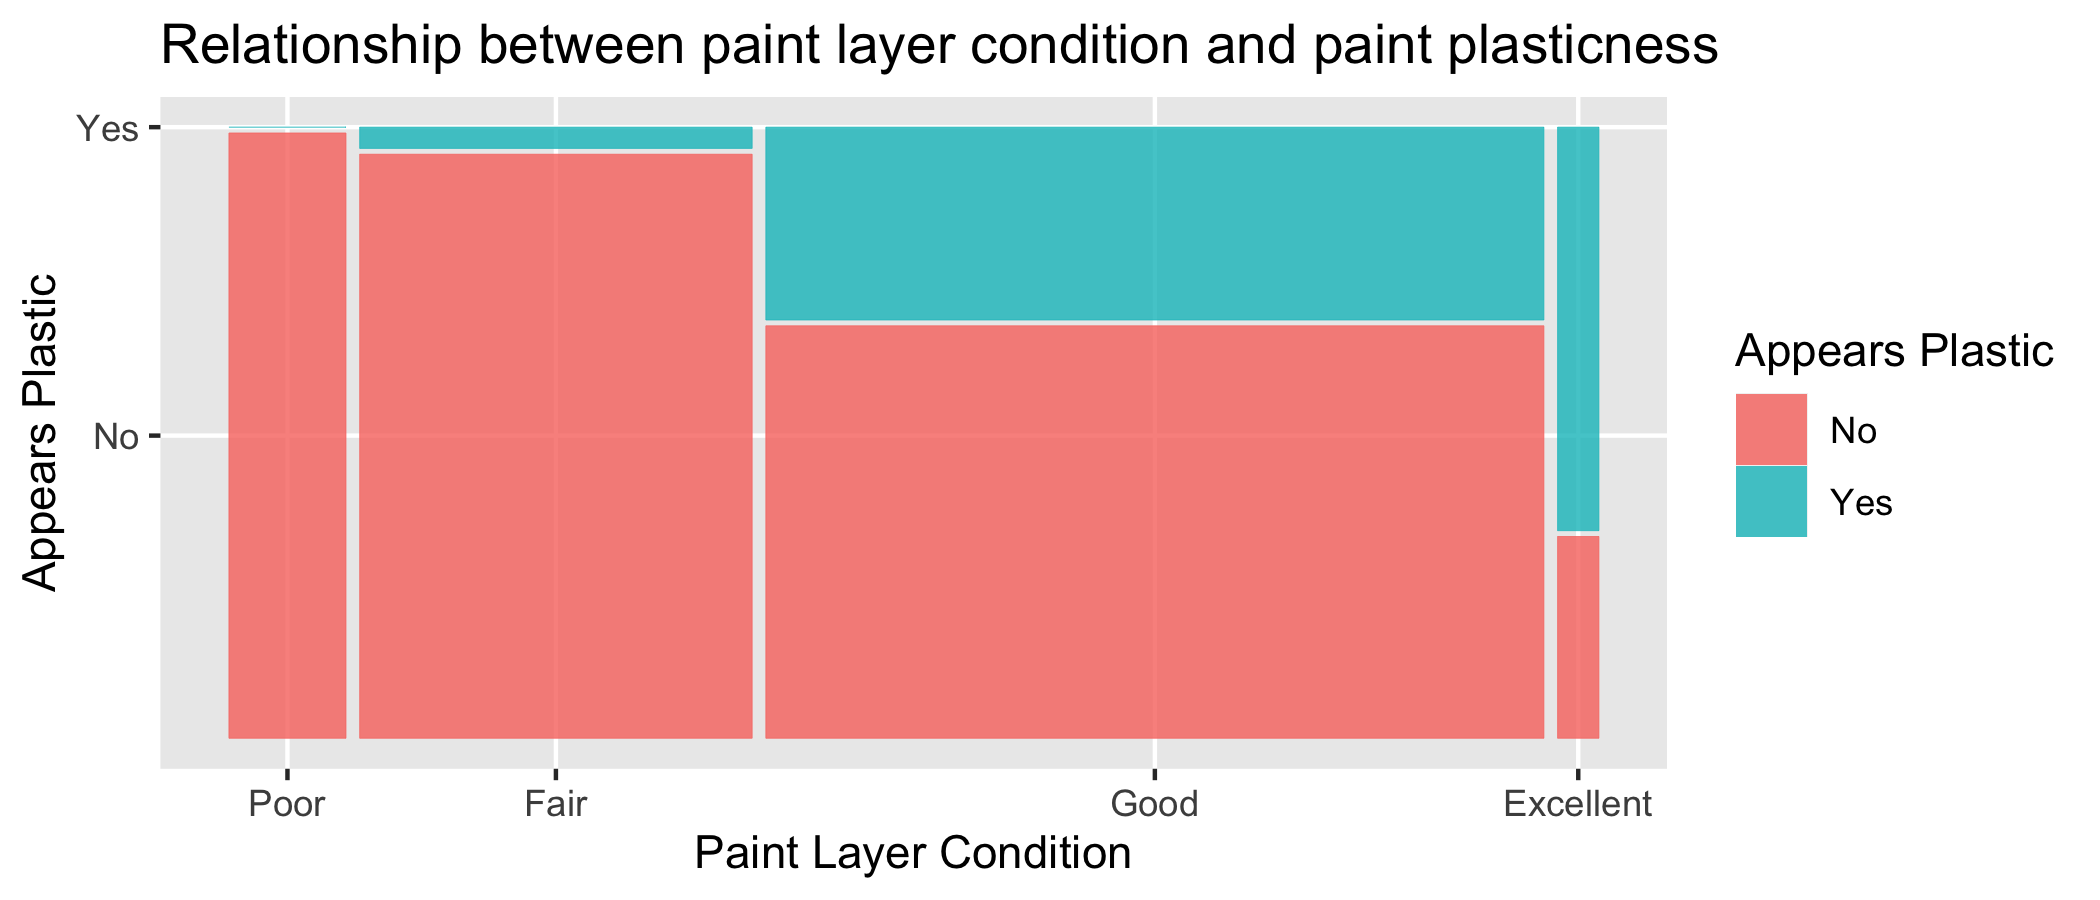
\includegraphics[scale=0.2]{images/pl_plastic.png}
    \caption{Relationship Between Paint Layer Condition and Paint Plasticness}
    \label{pl_plastic}
\end{figure}

\noindent On the other hand, it is a complete different story with plasticness of the paint. Figure \ref{pl_plastic} here visualises the relationship between paint layer condition and the plasticness of the painting, where we can see an decreasing trend of the proportion of paintings that does not appears to be plastic as the condition ratings increases from poor to excellent. And it is to be noted that similar relationship with the layer condition ratings could also be seen with support adherence of the paint layer.
\bigbreak
\noindent Furthermore, we aim to explore the relationship between some of the condition attributes that are non-independent, especially the relationship between cracking and it's associated attributes, as the client suggests.

\begin{figure}[H]
    \centering
    \includegraphics[scale=0.2]{images/dry_crack.png}
    \caption{Relationship Between Dry Cured and Paint Discolouration}
    \label{dry_crack}
\end{figure}

\noindent Figure \ref{dry_crack} above visualises the relationship between dry cured and paint crack. The height the boxes shows the condition proportion of paintings with paint crack given whether not the painting has dry cured condition. As we can see, under the studied samples, if the painting has dry cured condition, there is a higher chance it will has paint crack than those without. In fact, after computing the odds ratio, the odds of having paint crack for a painting with dry cured condition are about 2.5 times higher than paintings without dry cured condition.

\begin{figure}[H]
    \centering
    \captionsetup{justification=centering}
    \begin{minipage}{0.5\textwidth}
        \centering
        \includegraphics[width=1\textwidth]{images/plastic_crack.png} 
        \caption{Relationship Between Paint Crack and Paint Plasticness}
        \label{plastic_crack}
    \end{minipage}\hfill
    \begin{minipage}{0.5\textwidth}
        \centering
        \includegraphics[width=1\textwidth]{images/elastic_crack.png} 
        \caption{Relationship Between Paint Crack and Paint Elasticness}
        \label{elastic_crack}
    \end{minipage}
\end{figure}

\noindent To assess the relationship between paint cracking and paint plasticness, Figure \ref{plastic_crack} depicts, paintings without signs of plasticness has higher proportion of cracking present. While the proportion of cracking is much lower among those paintings with plasticness present. In contrast, the relationship of paint crack and paint elasticness is complete opposite as shown in Figure \ref{elastic_crack}.

\begin{figure}[H]
    \centering
    \includegraphics[scale=0.17]{images/accretion_crack.png}
    \caption{Relationship Between Paint Cracking and Paint Layer Accretion}
    \label{accretion_crack}
\end{figure}

\noindent Moreover, the relationship between paint cracking and paint layer accretion was shown in Figure \ref{accretion_crack}. It can be seen from the figure that the proportion of paintings with paint cracks are moderately higher among those with accretion in paint layer compare to those does not have accretion.

\subsection{Section Summary}
In this section, we presented the independence testing result of pairwise condition attributes for the three layers, namely, the paint support layer, the ground layer, and the paint layer. Additionally, mosaic plots were used to visualise the relationship between the dependent attributes. Unfortunately, we cannot test the association for higher-order contingency tables due to the small size of the dataset, some cells in the constructed contingency tables were not captured by the sample population, causing the Log-linear model to become saturated, producing an unreliable fit to the data. Additionally, throughout the discussion, we have been quite conservative in trying not to deduce the relationship between the attributes, as dependence does not imply causality. Therefore, a more detailed analysis, such as cohort and case-control studies, would be required to further establish causality between the condition attributes.

\section{Predictive Modelling of Missing Values}
In this section, we will be focusing on covering our approach to use machine learning models to predict some of the missing values from the dataset. More specifically, we tried to predict missing values for three features: \texttt{ground\_layer\_application}, \texttt{ground\_layer\_limit} and \texttt{ground\_layer\_thickness}. The first one specifies if the ground layer was applied by the artist or if it was already applied in an industrial way when the artist bought the canvas. The second feature states if the ground layer is only applied on the visible part of the canvas or if it goes to the side edges as well. Finally, the third one states if the ground layer is thick or not.

\subsection{Data Preprocessing for Prediction}
\subsubsection{One-Hot Encoding}
As discussed in the data cleaning section, most of the categorical attributes record the presence of a particular paint condition. Hence, these attributes were treated as binary attributes, corresponding to the presence (1) or absence (0) of a condition. Moreover, the One-Hot encoding method was applied to categorical variables with more than two levels, where one new binary attribute is added for each level in the original variable.

\subsubsection{Mutual Information for Feature Selection}
Once all the features we are interested in were either numerical or binary (we did not transform the Accession numbers or the artists with One-hot encoding), we then compute the mutual information (MI) between the features and the target variable. Mutual information is used to identify features that are well related to the target variable, which is based on the idea of knowing a variable will let us predict the target with more confidence, a higher MI score means higher dependency between the target and features.
\bigbreak
\noindent For each of the three features we tried to predict, we selected the 20 features that presented the highest mutual information score. We then fed several algorithms with these values.

\subsubsection{Data Splitting}
Supervised machine learning algorithms require the data to be splitted into a training and a testing set. We used \texttt{train\_test\_split} from the \texttt{sklearn} package to do it. However, by looking at the distribution of the data in Figure \ref{distribTrTe}, we could see the distribution of \texttt{ground\_layer\_limit} and \texttt{ground\_layer\_thickness} were biased and splitting at random could lead to an even more over-representation of the dominating category in the training set. This is why we used the \texttt{stratify} option when splitting. It consists in making sure the training set has all the possible categories represented with the same ratio as in the original population.

\begin{figure}[H]
\centering
\includegraphics[width=.5\textwidth]{images/distribApp.png}\hfill
\includegraphics[width=.5\textwidth]{images/distribLim.png} 
\\[\smallskipamount]
\includegraphics[width=.5\textwidth]{images/distribThic.png}\hfill
\caption{Distribution of each data set before the train/test split}
\label{distribTrTe}
\end{figure}

\subsection{Predictive Modelling}
We have chosen to use a Bernoulli Naive Bayes classifier as the baseline model. We hope that we would be able to improve the prediction performance as we introduce more advanced machine learning models. Given the small size of the dataset, neural network models were not used due to their high complexity; as we do not have enough data to produce an adequate fit, models will incorporate the noise of the samples leading to overfitting (high variance).

\subsubsection{Bernoulli Naive Bayes Classifier}
Bernoulli Naive Bayes is a classification model based on the Bayes Theorem. It assumes all attributes are generated from a \textit{Bernoulli} distribution, which is similar to our dataset, where 1 indicates the presence of a condition in the painting and 0 indicates the absence. Training is done by computing the prior probability of each class and the conditional probability of each attribute given the class. Classification is done by calculating the probability of a sample being each class, and the class with the highest posterior probability is the prediction outcome, and can be represented by the equation below. Although it is important to note that this classifier has a strong assumption of the attributes do not interact.

\begin{equation*}
    \hat{c} = \arg \max_{c_j\in C} \text{P}(c_j)\prod_{i}\text{P}(x_i\mid c_j)
\end{equation*}

\subsubsection{Random Forest Classifier}
Random Forest is an ensemble learning method for classification, it works by constructing multiple decision trees using different sets of bootstrap data (randomly sampled dataset, with replacement), which aims to reduce the correlation among the trees, so that trees can protect each other from their individual errors. Classification is done by aggregating the prediction of each individual tree, and the prediction outcome is the class with the highest vote.

\subsubsection{Logistic Regression}
A logistic regression is a statistical model which attempts to model the cumulative distribution function of a binary variable $Y$. It does it by assuming, if we are considering $N$ features as predictors, there exist a vector of parameters $\boldsymbol\beta = (\beta_i)_{0\leq i \leq N}$ such that for any set of features $\mathbf{X} =(1, \; x_1, \;  \ldots, \;  x_N)'$ :
\begin{equation*}
    p(Y=1) = \frac{1}{1 + \exp{\left(-\boldsymbol\beta'\mathbf{X}\right)}}
\end{equation*}

\noindent Unlike linear regression, there are no closed form solution for the parameters $\boldsymbol\beta$. Thus, parameters here are estimated by the method of coordinate descent.

\subsubsection{Stacking}
The last model that we implement is the stacking ensemble classifier, where the predictions of the previous classifier are given as input features for the meta-classifier. And the final prediction is done via majority voting.

\subsection{Model Evaluation and Suggestion}

\subsubsection{Hyperparameter Validation}
The logistic regression could take an extra argument when called: C, the inverse of the regularization strength. To find the best value for this parameter, we fitted several logisitc regressions for each of the features we wanted to predict with its complete non empty data set (the union of the training and the testing set). Each regression had a specific value of C that spaned from 0.01 to 100. For each of these models, we compared the training accuracy and we selected the value of C which yielded the best accuracy. Once this value selected, we fitted a new logistic regression with the training set only.
\bigbreak
\noindent Regarding the random forest, we had the freedom to specify several arguments: the number of trees, the maximum depth of each tree, the criterion to measure the quality of a split and the maximum number of features to look at when deciding for the best split. Choosing the best value for these tuning parameter was done by doing a grid search. This simply consists on testing every possible combination within a pool of potential values we gave as extra input. 

\subsubsection{Evaluation}
We can see in table \ref{Accuracies} the summary results of our models. The accuracies are overall pretty satisfying (all are above 0.75) but the testing sets are pretty small as we can see in the table \ref{table of counts}. This makes us think the holdout accuracies cannot be used as a base for a general result. Moreover, we can see for the logistic regression on \texttt{ground\_layer\_limit} the holdout accuracy was greater than the training accuracy. This is not that surprising considering the small size of the training and the testing datasets. It is especially true for this feature because the number of unspecified category was even larger than the size of the training set with only 81 training data points and 35 testing ones for 91 to predict.
 
\begin{table}[h]
\centering 
\begin{tabular}{c|c|c|c|}
     \multicolumn{2}{c}{} &  Training accuracy & Holdout accuracy \\
     \hline
     \multirow{3}{*}{\texttt{ground\_layer\_application}} & Naives Bayes & 0.852 & 0.821 \\
    \cline{2-4}
    & Random Froest & 1.0 & \textbf{0.839} \\
    \cline{2-4}
    & Logistic Regression & 0.852 & 0.821 \\
    \cline{2-4}
    & Stacking & 0.914 & \textbf{0.839}\\
    \hline
    \hline
    \multirow{3}{*}{\texttt{ground\_layer\_limit}} & Naives Bayes & 0.815 & 0.829 \\
    \cline{2-4}
    & Random Froest & 0.975 & 0.829 \\
    \cline{2-4}
    & Logistic Regression & 0.852 & \textbf{0.886} \\
    \cline{2-4}
    & Stacking & 0.922 & 0.821\\
    \hline
    \hline
    \multirow{3}{*}{\texttt{ground\_layer\_thickness}} & Naives Bayes & 0.830 & 0.769 \\
    \cline{2-4}
    & Random Froest & 0.989 & \textbf{0.846} \\
    \cline{2-4}
    & Logistic Regression & 0.875 & 0.795 \\
    \cline{2-4}
    & Stacking & 0.914 & 0.821\\
    \hline
\end{tabular}
\caption{Model Performance}
\label{Accuracies}
\end{table}


\begin{table}[h]
\centering 
\begin{tabular}{c|c|c|c|}
     & Training set & Testing set & To predict \\
     \hline
     \texttt{ground\_layer\_application}& 128 & 56 & 24\\
    \hline
    \texttt{ground\_layer\_limit}& 81 & 35 & 91\\
    \hline\texttt{ground\_layer\_thickness}& 88 & 39 & 80\\
    \hline
\end{tabular}
\caption{Size of the Different Datasets}
\label{table of counts}
\end{table}

\medbreak
\noindent The previous paragraph was focusing on the holdout accuracy. However we know this metric can be oversimplifying, this is why we kept trace the confusion matrices for every model and left them available in the appendix. We did not know enough domain knowledge to gain much insight with the matrices, this is why we are not doing some deep analysis of these matrices. Moreover, this part was more of an exercise for us since it was not requested by the client at all. We were still able to present the results to the client but they were of no interest for her, since it is not the main focus of the project.

%In general every algorithm performed well. But the Naive Bayes performed particularly well when looking at the Holdout accuracy.

%Two remarks were done nevertheless :
%\begin{itemize}
%    \item Some algorithms would predict only one class and still have a holdout accuracy superior than 0.6 because the dataset was very biased
%    \item Some algorithms presented a holdout accuracy higher than their training accuracy. This could have been caused by a discrepancy in the training/testing split of the data. This matter needs further investigation  \textcolor{red}{Phenomenon only for thickness and limit, for thickness almost same number of unspecified than training elets and for limit there are actually more unspecified than training ones} 
%\end{itemize}

\section{Conclusion and Future Work}
In this report, we have covered our approach and discussed the outcome on data preprocessing, interactive dashboard, independence testing for categorical data, and predictive modelling for missing values. As an achievement, our developed dashboard has been shared to the participating museums of the original study. Now both the client and the museums have access to the dashboard, they can base new work on it, trying to add new features for instance, if a new team happens to work on this project.
\bigbreak 
\noindent Regarding the independence testing result of the painting condition attributes, we are unable to deduce the causal effect between the conditions due to the limitation of the test as mentioned earlier. Therefore, one might consider to implement case control or cohort studies to further establish the causal relationship between two attributes. As for the models trained for missing value predictions, since the models were trained using limited samples, the data might not be a general representation of the overall population. We would not suggest using them for future predictions as the models could be highly biased. For future reference, if more samples can be included, models can be retrained to yield better generalisation.
\bigbreak
\noindent We have proposed last semester to map the relationship between artists and their commonly used painting materials. However, as we explored the dataset, most of the artists only contributes one to two paintings to the study. Thus, if more paintings from the artists were included, we could perhaps develop the relationship and connection between the artists and the used materials.
\bigbreak
\noindent Lastly, we have also proposed to identify the relationship between tropical climate and painting conditions. However, since the data was collected almost twenty years ago no detailed storage climate history could have been sourced. Therefore, for future references, if more detailed storage climate data can be found, the team working on this project can try to measure how different climate conditions affect paintings.

\newpage
\section{Appendix}
\subsection{Algorithms \& Pseudo-code}

\begin{algorithm}[H]
\SetAlgoLined
\KwInput{$D_I$: Dataframe of manually cleaned data \\ $L_{index}$ : A list of column indexes \\
colName: name of the feature}
\KwOutput{$D_O$: a single column Dataframe}
 $D_O:= \text{empty dataframe with one column named after colName}$\;
 $D_O\gets D_I[:, L_{index}[0]$\;
 \For{$index\:\:in\:\:L_{index}[1:]$}{
    $NewCat := D_I[:, index]$\;
    $nonEmptyNew :=$ the boolean serie telling if the cells of $NewCat$ are different from ""\;
    $nonEmptyExisting :=$ the boolean serie telling if the cells of $D_O$ are different from ""\;
  \eIf{colName = "ground\_layer\_application"}{
   $D_O[(nonEmptAddCat) \& (nonEmptExistingCat)]$ = "unsure";
   }{
   $D_O[(nonEmptAddCat) \& (nonEmptExistingCat)]$ = "both";
   }
   $D_O[(nonEmptAddCat) \& \lnot (nonEmptExistingCat)]$ = $NewCat[ \lnot (nonEmptExistingCat)]$;
}
$\textbf{Return: }D_O$
 \caption{fuseCategColumns}
 \label{fuseCat}
\end{algorithm}

\begin{algorithm}[H]
\SetAlgoLined
\KwInput{$D_I$: Dataframe of manually cleaned data \\ $L_{index}$ : list of the indexes of the columns we want to fuse, from the lower level to the highest \\
colName: name of the feature}
\KwOutput{$D_O$: a single column Dataframe}
 $D_O:= \text{empty dataframe with one column named after colName}$\;
 $level := 0$\;
 Fill $D_0$ with 0s\;
 \For{$index\:\:in\:\:L_{index}[1:]$}{
    $level \gets level + 1$\;
    $existsInOrigin :=$ the boolean serie telling if the cells of $NewCat$ are different from 0 and "NaN"\;
    $NaNInOrigin :=$ the boolean serie telling if the cells of $NewCat$ are "NaN"\;
    $nonZeroExisting :=$ the boolean serie telling if the cells of $D_O$ are different from 0\;
  
   $\left(D_O[(existsInOrigin) \& (nonZeroExisting)], D_O[(existsInOrigin) \& \lnot(nonZeroExisting)]\right) \gets  \left(
    \lceil \frac{D_O[(existsInOrigin) \& (nonZeroExisting)]+ level}{2}\rceil , level\right)$\;
   $D_0[NaNInOrigin] \gets Nan$\;
}
Replace 0 values of $D_0$ by NaN \;
Substract 1 to all the values of $D_0$\;

$\textbf{Return: }D_O$
 \caption{fuseOrdinalColumns}
 \label{fuseOrd}
\end{algorithm}
\newpage

\subsection{Confusion Matrices for the Predictive Modelling}

\begin{figure}[H]
\includegraphics[width=.5\textwidth]{images/matNBApp.png}\hfill
\includegraphics[width=.5\textwidth]{images/matRFApp.png} 
\\[\smallskipamount]
\includegraphics[width=.5\textwidth]{images/matLRApp.png}\hfill
\includegraphics[width=.5\textwidth]{images/matStackApp.png}\hfill
\caption{Confusion matrices for \texttt{ground\_layer\_application}}
\label{matApp}
\end{figure}

\begin{figure}[H]
\includegraphics[width=.5\textwidth]{images/matNBLim.png}\hfill
\includegraphics[width=.5\textwidth]{images/matRFLim.png} 
\\[\smallskipamount]
\includegraphics[width=.5\textwidth]{images/matLRLim.png}\hfill
\includegraphics[width=.5\textwidth]{images/matStackLim.png}\hfill
\caption{Confusion matrices for \texttt{ground\_layer\_limits}}
\label{matLim}
\end{figure}

\begin{figure}[H]
\includegraphics[width=.5\textwidth]{images/matNBThic.png}\hfill
\includegraphics[width=.5\textwidth]{images/matRFThic.png} 
\\[\smallskipamount]
\includegraphics[width=.5\textwidth]{images/matLRThic.png}\hfill
\includegraphics[width=.5\textwidth]{images/matStackThic.png}\hfill
\caption{Confusion matrices for \texttt{ground\_layer\_thickness}}
\label{matThic}
\end{figure}


\newpage
\subsection{Project Management}
\subsubsection{GitHub Repository}
Throughout the year, all our code and document were maintained with the following GitHub repository, \newline
\url{https://github.com/DS-Project-Group-7/Data-Science-Project}

\begin{figure}[H]
    \centering
    \includegraphics[scale=0.22]{images/github-repo.jpeg}
    \caption{Project Repository}
    \label{github-repo}
\end{figure}

\noindent For confidentiality and privacy concerns, all group members have mutually agreed not to share project files with outsiders, and access to the GitHub repository is limited to group members, project supervisor Vivek Katial, and our client Nicole Tse. Furthermore, two factor authentication is set up for our GitHub accounts.
\bigbreak
\noindent Branching is used throughout the project to maintain stability of the repository and isolates changes made to the code as shown in Figure \ref{github-branching}.

\begin{figure}[H]
    \centering
    \includegraphics[scale=0.46]{images/branching.png}
    \caption{GitHub Branching}
    \label{github-branching}
\end{figure}

\noindent Group member contributions to the repository are tracked using GitHub's built-in contribution log functionality as shown in Figure \ref{repo-contribution}.

\begin{figure}[H]
    \centering
    \includegraphics[scale=0.35]{images/repo-contribution.jpeg}
    \caption{Repository Contribution}
    \label{repo-contribution}
\end{figure}

\subsubsection{Project Task Tracking}
\begin{figure}[H]
    \centering
    \includegraphics[scale=0.3]{images/Trello_tracking.png}
    \caption{Trello Project Progress Tracking}
    \label{Trello_tracking}
\end{figure}
As a result of a year-long project, our team encountered that there were so many tasks to work on and track the status along with studying other subjects; Hence, we created the Trello template of tracking status into 4 steps consisting of To-do, Doing, Testing and Done. Then, we discussed the tasks and allocated tasks by volunteers. The result of our work is shown in Figure \ref{Trello_tracking}.
\bigbreak
\noindent One of the benefits of this approach is that everyone contributed their idea to prioritise the task and assign the task equally.

\subsubsection{Client and Supervisor Meeting Logs}
\begin{table}[H]
\resizebox{\textwidth}{!}{
\begin{tabular}{|l|l|l|l|}
\hline
\textbf{Week} & \textbf{Time} & \textbf{Hosts} & \textbf{Agenda} \\ \hline
Week 4 & 24/3/2022, 10:00 - 10:30 AM & Vivek Katial (Super) & \begin{tabular}[c]{@{}l@{}}- Kick-off meeting with the group supervisor\\ - Group member introduction\end{tabular} \\ \hline
Week 5 & 29/3/2022, 10:00 - 11:00 AM & \begin{tabular}[c]{@{}l@{}} Nicole Tse (Client)\\ Vivek Katial (Super)\end{tabular} & \begin{tabular}[c]{@{}l@{}}- Kick-off meeting with client \\ - Project plan discussion\end{tabular} \\ \hline
Week 6 & 7/4/2022 , 10:00 - 10:30 & Vivek Katial (Super) & - Project approach discussion with supervisor \\ \hline
Week 7 & 13/4/2022, 10:30 - 11:30 AM & Nicole Tse (Client) & \begin{tabular}[c]{@{}l@{}}- Question about literature\\ - Question about data and cleaning process \\ - R Shiny presentation \end{tabular} \\ \hline
Non-teaching period & 21/4/2022, 10:00 - 11:30 AM & Vivek Katial (Super) & \begin{tabular}[c]{@{}l@{}}- Data cleaning progress sharing\\ - Question about R Shiny\end{tabular}  \\ \hline
Week 9 & 5/5/2022, 11:00 - 11:30 PM & Vivek Katial (Super) & 
\begin{tabular}[c]{@{}l@{}}- Dashboard demo discussion\\ - Question about R Shiny \\ - Data cleaning progress sharing \end{tabular}  \\ \hline
Week 10 & 11/5/2022, 10:30 - 11:30 AM & Nicole Tse (Client) & \begin{tabular}[c]{@{}l@{}}- Presenting dashboard demo to client\\ - Question about dataset \\ - Data cleaning progress sharing \\ - Schedule for lab demonstration \end{tabular} \\ \hline
Week 11 & 18/5/2022, 10:30 - 11:30 AM & Nicole Tse (Client) & \begin{tabular}[c]{@{}l@{}}- Lab demonstration at Grimwade Centre\\ - Proposal for semester 2  \end{tabular} \\ \hline
Week 11 & 19/5/2022, 11:00 - 11:30 PM & Vivek Katial (Super) & \begin{tabular}[c]{@{}l@{}}- Semester 1 progress sharing\\ - Proposal for semester 2  \end{tabular} \\ \hline
\end{tabular}
}
\caption{Semester 1 Meeting Logs}
\end{table}

\begin{table}[H]
\resizebox{\textwidth}{!}{
\begin{tabular}{|l|l|l|l|}
\hline
\textbf{Week} & \textbf{Time} & \textbf{Hosts} & \textbf{Agenda} \\ \hline
Winter break & 20/7/2022, 1:00 - 2:00 PM & Nicole Tse (Client) & \begin{tabular}[c]{@{}l@{}}- Semester 2 kick-off meeting\\ - Discuss proposal for semester 2 \\ - Feedback on data cleaning \end{tabular} \\ \hline
Week 2 & 3/8/2022, 1:00 - 2:00 PM & Nicole Tse (Client) & \begin{tabular}[c]{@{}l@{}}- Data cleaning progress sharing \\ - Question about dashboard interface \\ - Ask about storage climate data \end{tabular} \\ \hline
Week 2 & 4/8/2022 , 10:00 - 10:30 AM & Vivek Katial (Super) & \begin{tabular}[c]{@{}l@{}}- Question about Shiny interface\\ - Dashboard implementation suggestion \end{tabular} \\ \hline
Week 5 & 26/8/2022, 10:30 - 11:30 AM & Vivek Katial (Super) & \begin{tabular}[c]{@{}l@{}}- Dashboard progress sharing and feedback\\ - Dashboard implementation suggestion \end{tabular} \\ \hline
Week 6 & 31/8/2022, 12:30 - 1:30 PM & Nicole Tse (Client) & \begin{tabular}[c]{@{}l@{}}- Dashboard progress sharing and feedback\\ - Additional question regarding the data \\ - Raise concern about storage climate data\end{tabular}  \\ \hline
Week 7 & 9/9/2022, 10:30 - 11:30 AM & Vivek Katial (Super) & \begin{tabular}[c]{@{}l@{}}- Dashboard progress sharing and feedback\\ - Dashboard implementation suggestion \\ - Discuss possible task after complete dashboard \end{tabular} \\ \hline
Week 8 & 14/9/2022, 12:30 - 1:30 PM & Nicole Tse (Client) & \begin{tabular}[c]{@{}l@{}}- Dashboard progress sharing and feedback \\ - Discuss idea on independence testing \\ - Discuss idea on missing value prediction\end{tabular} \\ \hline
Week 10 & 5/10/2022, 12:30 - 1:30 PM & Nicole Tse (Client) & \begin{tabular}[c]{@{}l@{}}- Dashboard progress sharing and feedback \\ - Independence testing progress and result sharing \\ - Predictive modeling progress and result sharing \\ - Project report progress sharing \end{tabular} \\ \hline
Week 10 & 7/10/2022, 10:30 - 11:30 AM & Vivek Katial (Super) & \begin{tabular}[c]{@{}l@{}}- Dashboard progress sharing and feedback \\ - Independence testing result sharing and discussion \\ - Predictive modeling result sharing and discussion \\ - Project report progress sharing \end{tabular} \\ \hline
Week 11 & 12/10/2022, 12:30 - 1:30 PM & Nicole Tse (Client) & \begin{tabular}[c]{@{}l@{}} - Finalising dashboard \\ - Independence testing result and limitation discussion \\ - Predictive modeling result sharing \\ - Discuss possible future work\end{tabular} \\ \hline
\end{tabular}
}
\caption{Semester 2 Meeting Logs}
\end{table}

Our group has scheduled fortnight meeting with both the supervisor and the client. Most of the meeting were held on zoom due to COVID-19 and the availability of location of group members. However, our group had to skip two meeting during August because the client was not be available.

\newpage
\subsection{Dashboard User Manual}
To access the dashboard as shown in Figure \ref{Login_Homepage_2}, the user requires username and password to access the dashboard (username: supanuthaa@gmail.com, password: SEADashboard07).

\begin{figure}[H]
    \centering
    \includegraphics[scale=0.5]{images/Polished_login.png}
    \caption{Login page}
    \label{Login_Homepage_2}
\end{figure}

\noindent Once the user access into the dashboard, the system redirect on the homepage as displayed in Figure \ref{dashboard_home_2}.

\begin{figure}[H]
    \centering
    \includegraphics[scale=0.25]{images/Dashboard Homepage Screenshot.png}
    \caption{Dashboard Homepage}
    \label{dashboard_home_2}
\end{figure}

\newpage
\begin{figure}[H]
    \centering
    \includegraphics[scale=0.5]{images/filter_option.png}
    \caption{Filter Option}
    \label{filter_2}
\end{figure}

\noindent Moreover, when user selected each component, the filter option is able to real-time filter information as user desired as shown in Figure \ref{filter_2}.
\begin{itemize}
    \item The museum group checkbox will dynamically filter the museum on the overall condition plot and the condition presents on each museum plot.
    \item The slider bar of time period will dynamically filter the decade of paintings for the whole plotting.
    \item The select input condition will dynamically filter the the condition presents on each museum plot.
    \item The select input two conditions will dynamically filter the the heat map for comparing two attributes plot on painting support tab as displayed in Figure \ref{two_con_filter_2}.
\end{itemize}

\begin{figure}[H]
    \centering
\includegraphics[scale=0.6]{images/two_con_filter.png}
    \caption{select input two conditions Filter Option}
    \label{two_con_filter_2}
\end{figure}
\newpage
\begin{figure}[H]
    \centering
\includegraphics[scale=0.35]{images/seach_top_data.png}
    \caption{Search function for the whole dataset}
    \label{seach_top_data_2}
\end{figure}

\noindent The data exploration tab was designed for dataset exploration. The search bar at top right allows the user to browse the specific key word a cleaned version of the dataset as shown in Figure \ref{seach_top_data_2}. In addition, a filter and search option have been added for each attribute, allowing the user to locate specific content by inputting a search string or selecting filter options as shown in Figure \ref{wood_type_search_2}.

\begin{figure}[H]
    \centering
\includegraphics[scale=0.35]{images/wood_type_search.png}
    \caption{Search function for each column attribute}
    \label{wood_type_search_2}
\end{figure}

\newpage
\printbibliography

\end{document}